\documentclass[a4paper,12pt]{article}
%\usepackage declarations should go here
\usepackage[utf8]{inputenc}
\setlength\parindent{0pt}
\usepackage[colorlinks]{hyperref}
\usepackage[table,xcdraw,svgnames,dvipsnames]{xcolor}
\usepackage{natbib} 
\usepackage[pdftex]{graphicx}
\usepackage[demo]{graphicx}
\usepackage{subcaption}
\usepackage{latexsym,amsmath,amssymb}
\usepackage{bm}
\usepackage{enumerate}
\usepackage{caption}
\graphicspath{{../pdf/}}
\captionsetup[figure]{labelfont={color=BrickRed}}
\captionsetup[table]{labelfont={color=BrickRed}}
\usepackage{url}
\usepackage{hyperref}
\usepackage[title]{appendix}
\usepackage{lmodern}
\usepackage{subcaption}
\usepackage{float}
\usepackage{setspace}
\usepackage{listings}
\usepackage[ruled,vlined,linesnumbered]{algorithm2e}

\tolerance=1
\emergencystretch=\maxdimen
\hyphenpenalty=10000
\hbadness=10000

% 
\usepackage[T
1]{fontenc}
\usepackage{parskip}
\usepackage{times}
\usepackage{zi4}
\usepackage[a4paper,left=3cm,right=3cm,top=3cm,bottom=3cm]{geometry}
%\usepackage{foundrysterlingbookosf}
\begin{document}
% Turn off page numbering until first section.
\pagenumbering{gobble}

\SetKwInput{KwInput}{Input}                % Set the Input
\SetKwInput{KwOutput}{Output}              % set the Output

%=============================================================
\definecolor{codegreen}{rgb}{0,0.6,0}
\definecolor{codegray}{rgb}{0.5,0.5,0.5}
\definecolor{codepurple}{rgb}{0.58,0,0.82}
\definecolor{backcolour}{rgb}{0.95,0.95,0.92}
 
\lstdefinestyle{mystyle}{
    backgroundcolor=\color{backcolour},   
    commentstyle=\color{codegreen},
    keywordstyle=\color{magenta},
    numberstyle=\tiny\color{codegray},
    stringstyle=\color{codepurple},
    basicstyle=\ttfamily\footnotesize,
    breakatwhitespace=false,         
    breaklines=true,                 
    captionpos=b,                    
    keepspaces=true,                 
    numbers=left,                    
    numbersep=5pt,                  
    showspaces=false,                
    showstringspaces=false,
    showtabs=false,                  
    tabsize=2
}
 
\lstset{style=mystyle}

%=============================================================
% define citation format
%=============================================================
\AtBeginDocument{
  \hypersetup{
    citecolor=CornflowerBlue,
    linkcolor=Red,   
    urlcolor=Magenta}}


% Title page - needs Stats_Logo.png
\begin{titlepage}
\begin{center}
\vspace{1cm}
\textsf{\Huge{University of Oxford \\}}
\vspace{1cm}
\begin{figure}[htb]
\centering

\includegraphics[scale=.8]{Stats_Logo.png}
\end{figure}
\vspace{2.0cm}
\Huge{High Dimensional Covariate Shift in Disease Risk Prediction\\}
\vspace{2.0cm}
\large{ by \\[14pt] Shuhan Liu \\[8pt]Wolfson  College} \\
\vspace{2.2cm}
\large{A dissertation submitted in partial fulfilment of the degree of Master of Science in Statistical Science.
} \\
\vspace{.5cm}
\large{\emph{Department of Statistics, 24--29 St Giles, \\Oxford, OX1 3LB}} \\
\vspace{1.0cm}
\large{September 2020} \\
\end{center}
\end{titlepage}
\clearpage


\begin{abstract}

Most statistical learning models are constructed on the assumption that the distribution of the training set is the same as the test set. Hence a model's performance on the training samples is regarded as an effective indicator for its performance in predicting test samples. However, this assumption is not held perfectly in practice. For example, in medical experiments, certain laboratory conditions and group control may be applied throughout the data collection, but may not be expected after being deployed outside lab. Also, samples may be drawn over a long period of time such that the old data is no longer representative to the more recent ones. This issue is known as covariate shift and can result in poor predictive performance. Covariate shift is common in genetics research where the majority of samples are of White ethnicity, but the results need to be employed to a wider range of populations. In this report, we investigate covariate shift adaption for high-dimensional data by reweighting training samples. We explore a range of supervised dimension reduction techniques, together with various density ratio estimation algorithms. Using an artificial dataset and the UK Biobank genotyping dataset, we compare the effectiveness of our proposed models to the ordinary unweighted model.

\end{abstract}
\clearpage
%\thispagestyle{empty}
\vspace*{2in}
\begin{center}
\textbf{Acknowledgements}
\end{center}

I would like to express my most sincere gratitude toward my supervisor, Dr. Brieuc Lehmann, who has always be reliable and responsive. He has continuously guided me throughout this project, replied to my queries with great patience and discussed in details about potential solutions. This project would not been done without his help and kindness.

I would also like to thank Yuqing Long, who has always been supportive and inspiring, I genuinely appreciate his help throughout the years. Also many thanks to Alex, Natalia and Weixi, the year in Oxford would have a lot less joy without them.

\clearpage

\tableofcontents
\clearpage

\pagenumbering{arabic}
%
%
%
%=============================================================
% Introduction
%=============================================================
%
%
%
\pagebreak
\section{Introduction} \label{introduction}
\subsection{Background}
The lack of ethnicity diversity in genome-wide association studies (GWASs) is well-documented. A study in 2009 showed that, 96\% of participants in GWASs are of European descendants [\cite{need2009next}]. Although this proportion dropped to 81\% in 2016, the increasing proportion of non-European participants are mostly Asian descendants. Remaining ancestries such as African, Hispanic \& Latin American and Arab \& Middle Eastern are still under-represented [\cite{popejoy2016genomics}]. Conducting GWASs in European ancestry was a practical starting point given the availability of samples and the limitations in funding, genotyping technologies, and analytic methods [\cite{peterson2019genome}]. However, the predictive power of GWAS findings and genetic diagnostic accuracy are weakened when transferring to other ancestries. A recent work examined the transferability of single-ancestry GWASs by calculating polygenic risk scores for eight well-studied phenotypes, finding that results from large-scale GWASs may have limited portability to other populations using standard approaches, and highlighting the need for generalised risk prediction methods [\cite{martin2017human}].

Recent methodological advances have leveraged patterns of global and local ancestry for improved variant association power [\cite{pasaniuc2011enhanced}] and enhanced identification of causal variants [\cite{zaitlen2010leveraging}]. However, there is limited success in identifying genome-wide significant genotypes associated with disease [\cite{martin2017human}]. There is an ongoing effort to disentangle the role of demography in heritability, linear mixed models and polygenic risk prediction [\cite{vilhjalmsson2015modeling}, \cite{carlson2013generalization}, \cite{martin2019clinical}]. With a similar objective, this report aims to explore the transfer learning methods which allow improved generalisation in ancestrally diverse populations, so that algorithms constructed on data of White individuals (mostly White British) can be deployed to other ethnic backgrounds.

Genotyping datasets exhibit some common characteristics. For example, each individual consists of a large number of variants, although only a small fraction of genotypes have a causal relationship to a specific phenotype. Genotypes from different populations also differ in distributions. Moreover, contiguous variants are likely to be correlated. A detailed illustration of these features is provided in Chapter \ref{Data} using the UK Biobank dataset.


%
%
%
%=============================================================
% Covariate Shift Correction
%=============================================================
%
%
%
\subsection{Covariate Shift Correction} \label{Covariate Shift Correction}
Given that in GWAS, an analysis may be carried out using samples that are mainly Europeans, then in practice are deployed to individuals from other populations that have very different features from the training samples. One possible remedy to improve the transferability is adopting a covariate shift correction [\cite{shimodaira2000improving}], introduced as follows:

Suppose we have $n_{tr}$ labelled training samples, denoted as $(x_{1}^{tr},y_{1}^{tr}), \cdots, (x_{n_{tr}}^{tr},y_{n_{tr}}^{tr}) \subseteq \mathcal{X} \times \mathcal{Y}$, with joint distribution $P_{XY}^{tr}$. The $n_{te}$ test samples are $(x_{1}^{te},y_{1}^{te}), \cdots, (x_{n_{te}}^{te},y_{n_{te}}^{te}) \subseteq \mathcal{X} \times \mathcal{Y}$, which are generated from $P_{XY}^{te}$. The labels $y_{te}$ are unobserved and we aim to predict them from features $x_{te}$. Covariate shift refers to the two following assumptions: (1) $P_{XY}^{tr} \neq P_{XY}^{te}$, (2) the distributions of labels conditional on features remain unchanged in both training and test domains, i.e.  $P_{Y|X}^{tr} = P_{Y|X}^{te}$, and therefore the joint distributions differ only via the marginal distributions $P_{X}^{tr}$ and $P_{X}^{te}$.

For a model $f \in \mathcal{F}$, let $L(f(x), y)$ be a point-wise loss function that measures the discrepancy between the true label $y$ and the predicted label $f(x)$. The goal is to minimise the risk under the test data distribution:
\begin{equation*}
    R^{te} = \mathbb{E}_{P^{te}_{XY}}[L(f(x), y)]   \text{.}
\end{equation*}
In practice, the joint distribution $P^{te}_{XY}$ is unknown, so the above risk is approximated by its empirical risk:
\begin{equation*}
    R^{te}_{emp} = \frac{1}{n_{tr}} \sum_{i = 1}^{n_{tr}}L(f(x_{i}^{tr}), y_{i}^{tr})
\end{equation*}
Under covariate shift, standard learning methods such as maximal likelihood estimation are no longer consistent, the same is true for the above empirical risk minimisation (in the sense that empirical risk does not converge to its optimal solution when the size of training samples tends to infinity) [\cite{shimodaira2000improving}]. Nonetheless, this inconsistency can be eliminated by expressing the empirical risk as an importance-weighted equation:
\begin{equation*}
    R^{te}_{emp}(\beta) = \frac{1}{n_{tr}} \sum_{i = 1}^{n_{tr}} \beta(x_{i}^{tr}) L(f(x_{i}^{tr}), y_{i}^{tr})
\end{equation*}
where $\beta(x) = \frac{P^{te}_{X}(x)}{P^{tr}_{X}(x)}$. This is demonstrated as follows:

\begin{align*} 
    R^{te} &= \int_{\mathcal{Y}}\int_{\mathcal{X}}{P^{te}_{XY} \cdot L(f(x), y)} dxdy \\
    &= \int_{\mathcal{Y}}\int_{\mathcal{X}}{P^{tr}_{XY} \cdot \frac{P^{te}_{XY}}{P^{tr}_{XY}} \cdot L(f(x), y)} dxdy\\
    &=  \int_{\mathcal{Y}}\int_{\mathcal{X}}{P^{tr}_{XY} \cdot \frac{P^{te}_{X}}{P^{tr}_{X}} \cdot L(f(x), y)} dxdy  \hspace{15pt} \text{from assumption (2)} \\
    & = \mathbb{E}_{P^{tr}_{XY}}[\beta(x) \cdot L(f(x), y)] \\
    &= R^{tr}(\beta) \\
    & \approx \frac{1}{n_{tr}} \sum_{i = 1}^{n_{tr}} \beta(x_{i}^{tr}) L(f(x_{i}^{tr}), y_{i}^{tr}) \text{.}
\end{align*}

Thus we can account for the the distribution difference between source and target domains by assigning each training sample a weight $\beta$, such that the re-weighted training data have the same distribution as the target domain samples. However, to carry out importance weighting, it is required to compute the density ratio $ \frac{P^{te}_{X}(x)}{P^{tr}_{X}(x)}$ which neither the numerator nor the denominator is given explicitly. A naive approach would be to estimate the training and test domain densities separately using flexible methods such as kernel density estimation [\cite{sheather1991reliable}], then derive the importance by taking ratio of the estimated densities. However, this approach is ineffective due to difficulty in estimating density accurately, especially in high dimensional domains [\cite{fishman2013monte}]. Moreover, division by an estimated quantity can lead to magnified estimation error [\cite{sugiyama2010dimensionality}]. 

Hence, it is imperative to avoid explicit estimation of distribution densities when learning the density ratio. Estimating the densities is more general than estimating the density ratios since once the former is computed accurately, the latter is easily derived, but not the vice versa [\cite{sugiyama2010dimensionality}]. In this report, we explore some algorithms to estimate this density ratio accurately by rewriting the ratio as a linear or non-linear model, without the need to know the distribution of features in either the training or test domains.

The outline of this report is as follows:
\begin{itemize}
	\item Chapter \ref{Importance Estimation} discusses the models for estimating the density ratio without explicitly computing the probability densities separately, then illustrates their performance in high dimensional feature space.
	\item Chapter \ref{Supervised Dimension Reduction} explains why supervised dimension reduction methods are more effective than unsupervised ones in our context, then explores a number supervised methods.
	\item Chapter \ref{Results} presents the results derived from experimenting on an artificial genotyping dataset and discusses the implications.
	\item Chapter \ref{Data} introduces the UK Biobank dataset, then provides the experiment results.
	\item Chapter \ref{Further Work} outlines some of future work directions.
	\item Chapter \ref{Conclusion} gives a summary of methods we used in this report and their performance.
\end{itemize}

\pagebreak
%
%
%
%=============================================================
% Importance Estimation
%=============================================================
%
%
%
\section{Importance Estimation} \label{Importance Estimation}
As mentioned in section \ref{Covariate Shift Correction}, to perform covariate shift correction, it is crucial to obtain accurate estimates of the density-ratio. Here, we focus on three density-ratio estimation techniques: Kernel Mean Matching (KMM), Unconstrained Least-squares Importance Fitting (uLSIF) and Kullback-Leibler Importance Estimation Procedure (KLIEP). Each of these methods formulates the density ratio as some linear or non-linear models and computes the ratio explicitly. Further details are shown in the following.

As before, assume we have $n_{tr}$ training samples $(x_{1}^{tr},y_{1}^{tr}), \cdots, (x_{n_{tr}}^{tr},y_{n_{tr}}^{tr}) \subseteq \mathcal{X} \times \mathcal{Y}$ and $n_{te}$ test samples $(x_{1}^{te},y_{1}^{te}), \cdots, (x_{n_{te}}^{te},y_{n_{te}}^{te}) \subseteq \mathcal{X} \times \mathcal{Y}$, drawn from distributions $P_{XY}^{tr}$ and $P_{XY}^{te}$ respectively. Also suppose the conditional distributions for the two domains are the same, i.e.  $P_{Y|X}^{tr} = P_{Y|X}^{te}$. We aim to find the true density ratio, expressed as $\beta(x) =  \frac{P^{te}_{X}(x)}{P^{tr}_{X}(x)}$.

%
%
%
%=============================================================
% KMM
%=============================================================
%
%
%
\subsection{Kernel Mean Matching (KMM)}
The moment matching method exploits fact that two distributions are equivalent if and only if all their moments are the same. For the true density ratio, we have $\beta(x){P^{tr}_{X}(x)} =  P^{te}_{X}(x)$, i.e. all moments of $\beta(x){P^{tr}_{X}(x)}$ and $P^{te}_{X}(x)$ match each other. Therefore, one simple implementation is to find the estimate of $\beta(x)$ such that first-order moment (i.e. the mean) of $\beta(x)P^{tr}_{X}(x)$, is compatible with $P^{te}_{X}(x)$ [\cite{gretton2009covariate}, \cite{sugiyama2010density}].

\subsubsection{Finite-order Approach}
The first moment implementation in finite order can be expressed as 
\begin{equation*}
\underset{\beta}{\operatorname{argmin}}\left\|\int \boldsymbol{x} \beta(\boldsymbol{x}) p_{\mathrm{tr}}(\boldsymbol{x}) \mathrm{d} \boldsymbol{x}-\int \boldsymbol{x} p_{\mathrm{te}}(\boldsymbol{x}) \mathrm{d} \boldsymbol{x}\right\|^{2}
\end{equation*}
where $\|\cdot\|$ represents the Euclidean norm. Given some non-linear function $\phi(\boldsymbol{x}): \mathbb{R}^{p} \rightarrow \mathbb{R}^{m}$, the non-linear variant of the above equation is expressed as 

\begin{align*}
\underset{\beta}{\operatorname{argmin}} & \left\|\int \phi{(\boldsymbol{x})} \beta(\boldsymbol{x}) p_{\mathrm{tr}}(\boldsymbol{x}) \mathrm{d} \boldsymbol{x}-\int \phi{(\boldsymbol{x})} p_{\mathrm{te}}(\boldsymbol{x}) \mathrm{d} \boldsymbol{x}\right\|^{2} \\
= \underset{\beta}{\operatorname{argmin}} & \left\|\int \phi(\boldsymbol{x}) \beta(\boldsymbol{x}) p_{\mathrm{tr}}(\boldsymbol{x}) \mathrm{d} \boldsymbol{x}\right\|^{2}-2\left\langle\int \boldsymbol{\phi}(\boldsymbol{x}) \beta(\boldsymbol{x}) p_{\mathrm{tr}}(\boldsymbol{x}) \mathrm{d} \boldsymbol{x}, \int \boldsymbol{\phi}(\boldsymbol{x}) p_{\mathrm{te}}(\boldsymbol{x}) \mathrm{d} \boldsymbol{x}\right\rangle + \text{constant}
\end{align*}

In practice, we only have a finite number of samples, thus the theoretical average is approximated with its sample average. Using the vector representation, the above equation can be shown as:
\begin{equation} \label{kmm_finite}
\hat{\boldsymbol{\beta}}_{\mathrm{tr}}:=\underset{\boldsymbol{\beta} \in \mathbb{R}^{n_{tr}} }{\operatorname{argmin}} \widehat{{MM}}(\boldsymbol{\beta}), \quad \text { where } \quad \widehat{{MM}}(\boldsymbol{\beta}):=\frac{1}{n_{\mathrm{tr}}^{2}} \boldsymbol{\beta}^{\top} \Phi_{\mathrm{tr}}^{\top} \Phi_{\mathrm{tr}} \boldsymbol{\beta}-\frac{2}{n_{\mathrm{tr}} n_{\mathrm{te}}} \boldsymbol{\beta}^{\top} \Phi_{\mathrm{tr}}^{\top} \Phi_{\mathrm{te}} 1_{n_{\mathrm{te}}}
\end{equation}
where $\boldsymbol{\Phi}_{\mathrm{te}}=\left( \boldsymbol{\phi} \left( \boldsymbol{x}_{1}^{\mathrm{te}} \right), \cdots, \boldsymbol{\phi} \left( \boldsymbol{x}_{n_{\mathrm{te}}}^{\mathrm{te}} \right) \right)$ and $\boldsymbol{\Phi}_{\mathrm{tr}}=\left( \boldsymbol{\phi}\left(\boldsymbol{x}_{1}^{\mathrm{tr}}\right), \ldots, \boldsymbol{\phi}\left(\boldsymbol{x}_{n_{\mathrm{tr}}}^{\mathrm{tr}}\right)\right)$, $MM$ stands for moment matching and $\widehat{MM}$ denotes its empirical estimate, $\mathbf{1}_{n}$ denotes the $n$-dimensional vector with all ones. 

The optimal solution of $\boldsymbol{\beta}$ can be found by solving $\widehat{{MM}}'(\boldsymbol{\beta}) = 0$. 
\begin{equation}
\frac{2}{n_{\mathrm{tr}}^{2}} \Phi_{\mathrm{tr}}^{\top} \Phi_{\mathrm{tr}} \beta-\frac{2}{n_{\mathrm{tr}} n_{\mathrm{te}}} \Phi_{\mathrm{tr}}^{\top} \Phi_{\mathrm{te}} 1_{n_{\mathrm{te}}}=0
\end{equation}
We must add a non-negative constraint to this optimisation problem: $\boldsymbol{\beta} \geq 0 $ since the ratios cannot be negative. We also impose upper bound $B$ such that $\boldsymbol{\beta} \leq B$, $B$ works as a regulariser that prevents the algorithm assigning very heavy weights to a few samples and causing a small effective sample size. This quadratic optimisation problem is linearly constrained and can be numerically solved by standard optimisation algorithms.

By using the algorithm we described, we can estimate the sample importance $\boldsymbol{\beta}$ at every data point in the training set. However, in order to make predictions on new samples out of our current dataset, we need to estimate the entire density ratio function, which can be done by assuming the following linear density-ratio model [\cite{kanamori2009condition}]
\begin{equation*}
\hat{\beta}(\boldsymbol{x})=\boldsymbol{\psi}(\boldsymbol{x})^{\top} \boldsymbol{\theta}
\end{equation*}
where $\boldsymbol{\psi}(\boldsymbol{x}): \mathbb{R}^{p} \rightarrow \mathbb{R}^{b}$ is some basis function that is assumed to be non-negative and $\boldsymbol{\theta} \in \mathcal{R}^{b}$ is some non-negative model parameter. Then we can express the density ratio as $\left(\beta\left({x}_{1}^{\mathrm{tr}}\right), \ldots, \beta\left({x}_{n_{\mathrm{tr}}}^{\mathrm{tr}}\right)\right)^{\top}=\boldsymbol{\Psi}_{\mathrm{tr}}^{\top} \boldsymbol{\theta}$ where $\boldsymbol{\Psi}_{\mathrm{te}}:=\left(\boldsymbol{\psi}\left(x_{1}^{\mathrm{te}}\right), \ldots, \boldsymbol{\psi}\left(x_{n_{\mathrm{te}}}^{\mathrm{te}}\right)\right)$. The optimisation problem is computed in terms of $\boldsymbol{\theta}$ and can be expressed as 
\begin{equation*}
\widehat{\boldsymbol{\theta}}:=\underset{\boldsymbol{\theta} \in \mathbb{R}^{b}}{\operatorname{argmin}}\left[\frac{1}{n_{\mathrm{tr}}^{2}} \boldsymbol{\theta}^{\top} \boldsymbol{\Psi}_{\mathrm{tr}} \boldsymbol{\Phi}_{\mathrm{tr}}^{\top} \boldsymbol{\Phi}_{\mathrm{tr}} \boldsymbol{\Psi}_{\mathrm{tr}}^{\top} \boldsymbol{\theta}-\frac{2}{n_{\mathrm{tr}} n_{\mathrm{te}}} \boldsymbol{\theta}^{\top} \boldsymbol{\Psi}_{\mathrm{tr}} \boldsymbol{\Phi}_{\mathrm{tr}}^{\top} \boldsymbol{\Phi}_{\mathrm{te}} \mathbf{1}_{n_{\mathrm{te}}}\right]
\end{equation*}
and the analytical solution for $\widehat{\boldsymbol{\theta}}$ is 

\begin{align*}
& \widehat{\boldsymbol{\theta}} =\frac{n_{tr}}{n_{te}}\left(\boldsymbol{\Psi}_{\mathrm{tr}} \boldsymbol{\Phi}_{\mathrm{tr}}^{\top} \boldsymbol{\Phi}_{\mathrm{tr}} \boldsymbol{\Psi}_{\mathrm{tr}}^{\top}\right)^{-1} \boldsymbol{\Psi}_{\mathrm{tr}} \boldsymbol{\Phi}_{\mathrm{tr}}^{\top} \boldsymbol{\Phi}_{\mathrm{te}} \mathbf{1}_{n_{\mathrm{te}}} \\
& \text {subject to} \hspace{25pt} \boldsymbol{\theta} \geq \mathbf{0}, \quad \text { and } \quad \boldsymbol{\theta} \leq B
\end{align*}

The upper bound $B$ can be found via cross-validation. The finite-order approach is simple and computationally efficient. However, it is not always consistent and does not guarantee to give the true density ratio. To ensure the consistency, we need to compare all the moments up to the infinite order and this motivates us to incorporate kernel methods into our current algorithm.

\subsubsection{Infinite-order Approach}
The infinite-order version, namely, the Kernel Mean Matching (KMM) method, uses a universal reproducing kernel $K\left(\boldsymbol{x}, \boldsymbol{x}^{\prime}\right)$ as a non-linear transformation. [\cite{gretton2009covariate}] shows that the solution of the optimal density ratio estimate can be derived by solving 
\begin{equation*}
\min _{r \in \mathcal{H}}\left\|\int K(x, \cdot) p_{\mathrm{te}}(x) \mathrm{d} x-\int K(x, \cdot) \beta(x) p_{\mathrm{tr}}(x) \mathrm{d} x\right\|_{\mathcal{H}}^{2}
\end{equation*}
Again, in practice with finite number of samples, this optimisation problem is reduced to 
\begin{equation*}
\min _{\boldsymbol{\beta} \in \mathbb{R}^{n_{tr}}}\left[\frac{1}{n_{\mathrm{tr}}^{2}} \boldsymbol{\beta}^{\top} \boldsymbol{K}_{\mathrm{tr}, \mathrm{tr}} \boldsymbol{\beta}-\frac{2}{n_{\mathrm{tr}} n_{\mathrm{te}}} \boldsymbol{\beta}^{\top} \boldsymbol{K}_{\mathrm{tr}, \mathrm{te}} \mathbf{1}_{n_{\mathrm{te}}}\right]
\end{equation*}
where $ \boldsymbol{K}_{\mathrm{tr}, \mathrm{tr}}$ and $ \boldsymbol{K}_{\mathrm{tr}, \mathrm{te}}$ are the two Gram matrices defined as $(\boldsymbol{K}_{\mathrm{tr}, \mathrm{tr}})_{ij} = K(x_{i}^{tr}, x_{j}^{tr})$ and $(\boldsymbol{K}_{\mathrm{tr}, \mathrm{te}})_{ij} = K(x_{i}^{tr}, x_{j}^{te})$
 
 By taking the first order derivative and setting it to zero, we obtain
 \begin{equation*}
\widehat{\boldsymbol{\beta}}_{\mathrm{tr}}=\frac{n_{\mathrm{tr}}}{n_{\mathrm{te}}} \boldsymbol{K}_{\mathrm{tr}, \mathrm{tr}}^{-1} \boldsymbol{K}_{\mathrm{tr}, \mathrm{te}} \mathbf{1}_{n_{\mathrm{te}}}
\end{equation*}
subject to the upper bound $B$ and lower bound 0 on ${\boldsymbol{\beta}}$. 

For new samples, we use the linear density ratio model, together with the kernel functions:
\begin{equation*}
\min _{\boldsymbol{\theta} \in \mathbb{R}^{b}}\left[\frac{1}{n_{\mathrm{tr}}^{2}} \boldsymbol{\theta}^{\top} \boldsymbol{\Psi}_{\mathrm{tr}} \boldsymbol{K}_{\mathrm{tr}, \mathrm{tr}} \boldsymbol{\Psi}_{\mathrm{tr}}^{\top} \boldsymbol{\theta}-\frac{2}{n_{\mathrm{tr}} n_{\mathrm{te}}} \boldsymbol{\theta}^{\top} \boldsymbol{\Psi}_{\mathrm{tr}} \boldsymbol{K}_{\mathrm{tr}, \mathrm{te}} \boldsymbol{1}_{n_{\mathrm{te}}}\right]
\end{equation*} 

subject to $\boldsymbol{\theta} \geq 0 $ and $\boldsymbol{\theta} \leq B$.

The KMM method is always consistent as long as the reproducing kernels we choose are universal. Also, it is formulated as a convex quadratic programming problem, which always leads to a unique global solution. However, its performance heavily depends on the kernel we choose and there is no reliable method to tune the kernel parameters, for example, the kernel width in a Gaussian kernel. This is because we cannot in practice find a Gaussian width that fits all moments well and hence standard methods such as cross-validation are ineffective. One practical strategy uses the median distance between the samples as the Gaussian bandwidth [\cite{smola1998learning}], although there is lack of justification for this heuristic. 

%
%
%
%=============================================================
% KLIEP
%=============================================================
%
%
%
\subsection{Kullback-Leibler Importance Estimation Procedure (KLIEP)}
The Kullback-Leibler Importance Estimation Procedure (KLIEP) is based on the minimisation of the Kullback-Leibler divergence between the distribution of reweighed training features and the distribution of test features. Compared to KMM, one noticeable advantage of KLIEP is that its model selection (such as choosing kernel parameters) can be carried out via cross-validation procedure, thus leaving no untuned parameter. This technique is introduced as follows [\cite{tsuboi2009direct}, \cite{sugiyama2010density}].

Similar to KMM, we first rewrite the density ratio as a linear model 
\begin{equation} \label{ratio appro}
\hat{\beta}(\boldsymbol{x})=\boldsymbol{\psi}(\boldsymbol{x})^{\top} \boldsymbol{\theta}
\end{equation}
where $\boldsymbol{\psi}(\boldsymbol{x}): \mathbb{R}^{p} \rightarrow \mathbb{R}^{b}$ is some basis function and $\boldsymbol{\theta} \in \mathcal{R}^{b}$ is the model parameter, assuming both $\boldsymbol{\theta}$ and $\boldsymbol{\psi}(\boldsymbol{x})$ to be non-negative.
We learn the parameter $\boldsymbol{\theta}$ such that the KL divergence between $\hat{\beta}(x){P^{tr}_{X}(x)}$ and $P^{te}_{X}(x)$ is minimised.
\begin{align*}
\mathrm{KL}\left[p_{\mathrm{te}}(\boldsymbol{x}) \| \hat{\beta}(\boldsymbol{x})p_{\mathrm{tr}}(\boldsymbol{x})\right] &=\int_{\mathcal{X}} p_{\mathrm{te}}(\boldsymbol{x}) \log \frac{p_{\mathrm{te}}(\boldsymbol{x})}{p_{\mathrm{tr}}(\boldsymbol{x}) \hat{\beta}(\boldsymbol{x})} d \boldsymbol{x} \\
&=\int_{\mathcal{X}} p_{\mathrm{te}}(\boldsymbol{x}) \log \frac{p_{\mathrm{te}}(\boldsymbol{x})}{p_{\mathrm{tr}}(\boldsymbol{x})} d \boldsymbol{x}-\int_{\mathcal{X}} p_{\mathrm{te}}(\boldsymbol{x}) \log \hat{\beta}(\boldsymbol{x}) d \boldsymbol{x}
\end{align*}
The first term is independent of $\hat{\beta}(\boldsymbol{x})$ and thus can be ignored from our optimisation problem. For the second term, we denote it as $J_{\mathrm{KLIEP}}$ 
\begin{equation*} 
J_{\mathrm{KLIEP}}=\int_{\mathcal{X}} p_{\mathrm{te}}(\boldsymbol{x}) \log \hat{\beta}(\boldsymbol{x}) d \boldsymbol{x}
\end{equation*}

Since the population distribution is usually unknown, in practice we approximate this quantity using its empirical value:
\begin{align} \label{kliep_obj}
\widehat{J_{\mathrm{KLIEP}}} &= \frac{1}{N_{\mathrm{te}}} \sum_{\boldsymbol{x} \in \mathcal{X}_{\mathrm{te}}} \log \hat{\beta}(\boldsymbol{x})\\
& = \sum_{\boldsymbol{x} \in \mathcal{X}_{\mathrm{te}}} \log \left(\boldsymbol{\psi}(\boldsymbol{x})^{\top} \boldsymbol{\theta} \right) \hspace{50pt} \text{from equation (\ref{ratio appro})}
\end{align}

We aim to maximise equation \ref{kliep_obj} in order to minimise KL divergence. Therefore, the optimisation problem is formulated as
\begin{align*}
& \underset{\boldsymbol{\theta}}{\operatorname{maximize}} \sum_{\boldsymbol{x} \in \mathcal{X}_{\mathrm{te}}} \log \left(\boldsymbol{\psi}(\boldsymbol{x})^{\top} \boldsymbol{\theta} \right) \\
& \text{subject to} \sum_{\boldsymbol{x} \in \mathcal{X}_{\mathrm{tr}}}  \boldsymbol{\psi}(\boldsymbol{x})^{\top} \boldsymbol{\theta} = N_{\mathrm{tr}} \hspace{15pt} \text{and} \hspace{15pt}\boldsymbol{\theta} \geq \mathbf{0} 
\end{align*}
$\boldsymbol{\theta} \geq \mathbf{0}$ ensures the density-ratio estimates are non-negative. The first constraint is from the fact that the probability density function ${p}_{\mathrm{te}}(\boldsymbol{x})$ integrates to 1, i.e.
\begin{align*}
1&=\int_{\mathcal{X}} {p}_{\mathrm{te}}(\boldsymbol{x}) d \boldsymbol{x} \\
&=\int_{\mathcal{X}} p_{\mathrm{tr}}(\boldsymbol{x}) \hat{\beta}(\boldsymbol{x}) d \boldsymbol{x} \\
& \approx \frac{1}{N_{\mathrm{tr}}} \sum_{\boldsymbol{x} \in \mathcal{X}_{\mathrm{tr}}} \hat{\beta}(\boldsymbol{x}) \hspace{15pt} \text{approximated by its empirical value} \\
& = \boldsymbol{\psi}(\boldsymbol{x})^{\top} \boldsymbol{\theta} \hspace{50pt} \text{from equation (\ref{ratio appro})}
\end{align*}
This is a convex optimisation problem and hence a global optimum is guaranteed. The solution can be obtained via iteratively applying gradient ascent and checking whether the constraints are satisfied at each iteration. The algorithm is illustrated using the following pseudo-code:

\begin{algorithm}[H]
\SetAlgoLined
 \KwInput{Data samples $D^{\mathrm{te}}=\left\{\boldsymbol{x}_{i}^{\mathrm{te}}\right\}_{i=1}^{n_{\mathrm{te}}}$ and $D^{\mathrm{tr}}=\left\{\boldsymbol{x}_{j}^{\mathrm{tr}}\right\}_{j=1}^{n_{\mathrm{tr}}}$ and basis function $\psi(\boldsymbol{x})$.}
 \KwOutput{The density ratio estimator $\hat{\beta}(\boldsymbol{x})$.}
 $\boldsymbol{\Psi}_{te} \longleftarrow\left(\boldsymbol{\psi}\left(\boldsymbol{x}_{1}^{te}\right), \ldots, \boldsymbol{\psi}\left(\boldsymbol{x}_{n_{te}}^{\mathrm{te}}\right)\right)^{\top}$ \;
 $\bar{\boldsymbol{\psi}}_{\mathrm{tr}} \longleftarrow \frac{1}{n_{\mathrm{tr}}} \sum_{j=1}^{n_{\mathrm{tr}}} \psi\left(\boldsymbol{x}_{j}^{\mathrm{tr}}\right)$ \;
 Initialize $\boldsymbol{\theta}\left(>\mathbf{0}\right)$ and $\varepsilon(0<\varepsilon \ll 1)$ \;
 \Repeat{convergence}{
 $\boldsymbol{\theta} \longleftarrow \boldsymbol{\theta}+\varepsilon \boldsymbol{\Psi}_{\mathrm{te}}^{\top}\left(\mathbf{1}_{n_{\mathrm{te}}} / \boldsymbol{\Psi}_{\mathrm{te}} \boldsymbol{\theta}\right)$ \tcp*{gradient ascent} \
 $\boldsymbol{\theta} \leftarrow \boldsymbol{\theta}+\left(1-\overline{\boldsymbol{\psi}}_{\mathrm{tr}}^{\top} \boldsymbol{\theta}\right) \overline{\boldsymbol{\psi}}_{\mathrm{tr}} /\left(\overline{\boldsymbol{\psi}}_{\mathrm{tr}}^{\top} \overline{\boldsymbol{\psi}}_{\mathrm{tr}}\right)$ \tcp*{Constraint satisfaction} \
 $\boldsymbol{\theta} \leftarrow \max \left(\mathbf{0}, \boldsymbol{\theta}\right)$ \tcp*{Constraint satisfaction} \
 $\boldsymbol{\theta} \longleftarrow \boldsymbol{\theta} /\left(\bar{\boldsymbol{\psi}}_{\mathrm{tr}}^{\top} \boldsymbol{\theta}\right)$ \tcp*{Constraint satisfaction}}
 $\widehat{\beta}(\boldsymbol{x}) \longleftarrow \boldsymbol{\psi}(\boldsymbol{x})^{\top} \boldsymbol{\theta}$
\caption{KL Importance Estimation Procedure}
\end{algorithm}

\subsubsection{Model Selection by Cross-validation}
The performance of KLIEP depends on the choice of the basis functions $\psi(\boldsymbol{x})$ as well as the parameters of the basis functions. Since the only constraint on the basis function is its non-negativeness, one reasonable choice is to use a Gaussian kernel 
\begin{equation*}
\beta(\boldsymbol{x})=\sum_{\ell=1}^{n_{\mathrm{te}}} \theta_{\ell} K\left(\boldsymbol{x}, \boldsymbol{x}_{\ell}^{\mathrm{te}}\right)
\end{equation*}
Notice that we only use the test set data as centres of the Gaussian kernel. This is because $\beta(\boldsymbol{x})$ tends to have large values if $P_{X}^{te}(x)$ is large and $P^{te}_{X}(x)$ is small, while $\beta(\boldsymbol{x})$ tends to be zero if the opposite. Thus a small number of kernels is needed in the target region that is small even close to 0 and a larger number of kernels required when the values at the target region is large. This choice may therefore achieve a more reasonable allocation of kernels. Furthermore, for the sake of computational efficiency when the test set sample size is large, it is possible to draw a random subset from$\{x_{i}^{te}\}_{i=1}^{n_{te}}$ as the Gaussian centres rather than using the entire dataset.

We can hence choose the model that maximises $J_{KLIEP}$. For different models (e.g. models with different Gaussian kernel width), the values of $J_{KLIEP}$ can be approximated via cross-validation. To be specific, we split the test set samples $\boldsymbol{X}_{te}$ into $T$ folds $\{\boldsymbol{X}_{te}^{t}\}_{t = 1}^{T}$, then compute the estimated density ratios $\hat{\beta}^{t}(\boldsymbol{x})$ from $\left\{\boldsymbol{X}_{\text {te }}^{k}\right\}_{k \neq t}^{T}$ and estimate the $J_{KLIEP}$ score using
\begin{equation*}
\hat{J}_{\mathrm{KLIEP}}^{t}=\frac{1}{\left|\boldsymbol{X}_{\mathrm{te}}^{t}\right|} \sum_{x \in \boldsymbol{X}_{\mathrm{te}}^{\mathrm{t}}} \hat{\beta}^{t}(\boldsymbol{x})
\end{equation*}
We repeat this procedure for each fold and each model, then select the one which has the maximum average $\widehat{J_{\mathrm{KLIEP}}}$ across all the folds. The pseudo-code for this cross-validation is given as follows:

\begin{algorithm}[H]
\SetAlgoLined
\KwInput{Data samples $D^{\mathrm{te}}=\left\{\boldsymbol{x}_{i}^{\mathrm{te}}\right\}_{i=1}^{n_{\mathrm{te}}}$ and $D^{\mathrm{tr}}=\left\{\boldsymbol{x}_{j}^{\mathrm{tr}}\right\}_{j=1}^{n_{\mathrm{tr}}}$ and basis function $\psi(\boldsymbol{x})$.}
 \KwOutput{The density ratio estimator $\hat{\beta}(\boldsymbol{x})$.}
 Split $D^{\mathrm{te}}=\left\{\boldsymbol{x}_{i}^{\mathrm{te}}\right\}_{i=1}^{n_{\mathrm{te}}}$ into $T$ disjoint subsets $\{\boldsymbol{X}_{te}^{t}\}_{t = 1}^{T}$\;
 \For{Model $m = 1, \cdots, M$}{
 \For{each fold $t = 1, \cdots, T$}{
 $\hat{\beta}_{t}(\boldsymbol{x}) \leftarrow \operatorname{KLIEP}\left(\left\{\boldsymbol{X}_{\text {te }}^{k}\right\}_{k \neq t}^{T}, \boldsymbol{X}^{\mathrm{tr}}, \boldsymbol{\psi}(\boldsymbol{x})\right)$ \;
 $\widehat{\mathrm{J_{KLIEP}}}^{t}(m) \longleftarrow \frac{1}{\left|\mathcal{X}_{l}^{\mathrm{te}}\right|} \sum_{\boldsymbol{x} \in \boldsymbol{X}_{t}^{\mathrm{te}}} \log \widehat{\beta}_{t}(\boldsymbol{x})$} 
 $\widehat{\mathrm{J_{KLIEP}}}(m) \longleftarrow \frac{1}{T} \sum_{t=1}^{T} \widehat{\mathrm{J_{KLIEP}}}^{t}(m)$}
 $\hat{m} \longleftarrow \operatorname{argmax}_{m} \widehat{\mathrm{J_{KLIEP}}}(m)$ \;
 $\widehat{\beta}(\boldsymbol{x}) \longleftrightarrow \operatorname{KLIEP}\left(D^{\mathrm{te}}, D^{\mathrm{tr}}, \boldsymbol{\psi}_{\widehat{m}}(\boldsymbol{x})\right)$
\caption{cross-validation for KLIEP}
\end{algorithm}

%
%
%
%=============================================================
% uLSIF
%=============================================================
%
%
%
\subsection{Unconstrained Least-square Importance Fitting (uLSIF)}
Unconstrained Least-square Importance Fitting (uLSIF) [\cite{yamada2013relative}] is similar to KLIEP except the former aims to minimise the squared error rather than the KL divergence. Again, we assume the following linear model for the density ratio 
\begin{equation*}
\hat{\beta}(\boldsymbol{x})=\boldsymbol{\psi}(\boldsymbol{x})^{\top} \boldsymbol{\theta}
\end{equation*}
where $\boldsymbol{\psi}(\boldsymbol{x}): \mathbb{R}^{p} \rightarrow \mathbb{R}^{b}$ is some non-negative basis function and $\boldsymbol{\theta} \in \mathcal{R}^{b}$ is the non-negative model parameter.

We learn the parameters $\boldsymbol{\theta} \in \mathcal{R}^{b}$ in this linear model such that the squared error $J_{uLSIF}$ is minimised:

\begin{align*}
J_{uLSIF}(\boldsymbol{\theta}) &:=\frac{1}{2} \int_{\mathcal{X}}(\widehat{\beta}(\boldsymbol{x})-\beta(\boldsymbol{x}))^{2} p_{\mathrm{tr}}(\boldsymbol{x}) d \boldsymbol{x} \\
&=\frac{1}{2} \int_{\mathcal{X}_{tr}} \widehat{\beta}(\boldsymbol{x})^{2} p_{\mathrm{tr}}(\boldsymbol{x}) d \boldsymbol{x}-\int_{\mathcal{X}_{te}} \widehat{\beta}(\boldsymbol{x}) p_{\mathrm{te}}(\boldsymbol{x}) d \boldsymbol{x}+\frac{1}{2} \int_{\mathcal{X}_{te}} \beta(\boldsymbol{x}) p_{\mathrm{te}}(\boldsymbol{x}) d \boldsymbol{x}
\end{align*}

The last component this equation does not contain $\widehat{\beta}$ and hence can be ignored in our optimisation problem. We aim to minimise
\begin{equation*}
J(\boldsymbol{\theta}):=\frac{1}{2} \int_{\mathcal{X}_{tr}} \widehat{\beta}(\boldsymbol{x})^{2} p_{\mathrm{tr}}(\boldsymbol{\beta}) d \boldsymbol{x}-\int_{\mathcal{X}_{te}} \widehat{\beta}(\boldsymbol{x}) p_{\mathrm{te}}(\boldsymbol{x}) d \boldsymbol{x}
\end{equation*}

In practice, we replace the expectations in the above equation by their empirical averages. Ten the objective equation can then be expressed as

\begin{align*}
\widehat{J}_{uLSIF}(\boldsymbol{\theta}) &:=\frac{1}{2 n_{\mathrm{tr}}} \sum_{i=1}^{n_{\mathrm{tr}}} \widehat{\beta}\left({\boldsymbol{x}}_{i}^{\mathrm{tr}}\right)^{2}-\frac{1}{n_{\mathrm{te}}} \sum_{j=1}^{n_{\mathrm{te}}} \widehat{\beta}\left({\boldsymbol{x}}_{j}^{\mathrm{te}}\right) \\
&=\frac{1}{2} \sum_{\ell, \ell^{\prime}=1}^{b} \theta_{\ell} \theta_{\ell^{\prime}}\left(\frac{1}{n_{\mathrm{tr}}} \sum_{i=1}^{n_{\mathrm{tr}}} \psi_{\ell}\left({\boldsymbol{x}}_{i}^{\mathrm{tr}}\right) \psi_{\ell^{\prime}}\left({\boldsymbol{x}}_{i}^{\mathrm{tr}}\right)\right)-\sum_{\ell=1}^{b} \theta_{\ell}\left(\frac{1}{n_{\mathrm{te}}} \sum_{j=1}^{n_{\mathrm{te}}} \psi_{\ell}\left({\boldsymbol{x}}_{j}^{\mathrm{te}}\right)\right) \\
&=\frac{1}{2} \boldsymbol{\theta}^{\top} \widehat{\boldsymbol{H}} \boldsymbol{\theta}-\widehat{\boldsymbol{h}}^{\top} \boldsymbol{\theta}
\end{align*}
 
where $\widehat{\boldsymbol{H}}$ is the $b \times b$ matrix with the $\left(\ell, \ell^{\prime}\right)$-th element equivalent to
\begin{equation*}
\widehat{H}_{\ell, \ell^{\prime}}:=\frac{1}{n_{\mathrm{tr}}} \sum_{i=1}^{n_{\mathrm{tr}}} \psi_{\ell}\left(\widehat{\boldsymbol{u}}_{i}^{\mathrm{tr}}\right) \psi_{\ell^{\prime}}\left(\widehat{\boldsymbol{u}}_{i}^{\mathrm{tr}}\right)
\end{equation*}
and $\widehat{\boldsymbol{h}}$ is the $b$-dimensional vector with the $\ell$-th element being
\begin{equation*}
\widehat{h}_{\ell}:=\frac{1}{n_{\mathrm{te}}} \sum_{j=1}^{n_{\mathrm{te}}} \psi_{\ell}\left({\boldsymbol{x}}_{j}^{\mathrm{te}}\right)
\end{equation*}

Now we can formulate the optimisation problem as follows:
\begin{equation} \label{ulsif_reg}
\widetilde{\boldsymbol{\theta}}:=\underset{\boldsymbol{\theta} \in \mathbb{R}^{b}}{\operatorname{argmin}}\left[\frac{1}{2} \boldsymbol{\theta}^{\top} \widehat{\boldsymbol{H}} \boldsymbol{\theta}-\widehat{\boldsymbol{h}}^{\top} \boldsymbol{\theta}+\frac{\lambda}{2} \boldsymbol{\theta}^{\top} \boldsymbol{\theta}\right]
\end{equation}
subject to $\boldsymbol{\theta}$ being non-negative. Here we add a regularisation term $\frac{\lambda}{2} \boldsymbol{\theta}^{\top} \boldsymbol{\theta}$ to prevent the algorithm assigning very large weights to a small number of samples, with $\lambda$ controlling the strength of the regularisation. By computing the first derivative of this equation and setting it to 0, we obtain the optimal solution as
\begin{equation*}
\widetilde{\boldsymbol{\theta}} = \left(\widehat{\boldsymbol{H}}+\lambda \boldsymbol{I}_{b}\right)^{-1} \widehat{\boldsymbol{h}}
\end{equation*}
To satisfy the non-negativity constraint on $\boldsymbol{\theta}$, we express the solution of $\widehat{\boldsymbol{\theta}}$ as
\begin{equation*}
\widehat{\boldsymbol{\theta}} = \text{max}\left( 0, \widetilde{\boldsymbol{\theta}} \right)
\end{equation*}


\subsubsection{Leave-one-out Cross-validation (LOOCV)}
As with KMM and KLIEP, the performance of uLSIF is affected by the choice of the basis functions and in practice, it is reasonable to use a Gaussian kernel as the basis function. To select the Gaussian width of the kernel as well as the regularisation parameter $\lambda$ in equation \ref{ulsif_reg}, we employ leave-one-out cross-validation (LOOCV). 

Denote $n:=\min \left(n_{\text {tr }}, n_{\mathrm{te}}\right)$. We hold out $\widehat{\boldsymbol{u}}_{k}^{\mathrm{tr}}$ and $\widehat{\boldsymbol{u}}_{k}^{\mathrm{te}}(k=1,2, \ldots, n)$ simultaneously in each iteration of the LOOCV procedure. Suppose that $\widehat{\beta}^{(-k)}(\boldsymbol{x})$ is the estimate of the density ratio computed from samples without $\widehat{\boldsymbol{u}}_{k}^{\mathrm{tr}}$ and $\widehat{\boldsymbol{u}}_{k}^{\mathrm{te}}$, then we can write the LOOCV score as 
\begin{equation*}
\widehat{J}_{\mathrm{LOOCV}}=\frac{1}{n} \sum_{k=1}^{n}\left[\frac{1}{2}\left(\widehat{\beta}^{(-k)}\left({\boldsymbol{x}}_{k}^{\mathrm{tr}}\right)\right)^{2}-\widehat{\beta}^{(-k)}\left({\boldsymbol{x}}_{k}^{\mathrm{te}}\right)\right]
\end{equation*}

The LOOCV procedure is demonstrated using the pseudo code shown in Algorithm \ref{ulsif algo}.

\begin{algorithm}
\SetAlgoLined
\KwInput{Data samples $D^{\mathrm{te}}=\left\{\boldsymbol{x}_{i}^{\mathrm{te}}\right\}_{i=1}^{n_{\mathrm{te}}}$ and $D^{\mathrm{tr}}=\left\{\boldsymbol{x}_{j}^{\mathrm{tr}}\right\}_{j=1}^{n_{\mathrm{tr}}}$ and basis function $\psi(\boldsymbol{x})$.}
\KwOutput{The density ratio estimator $\hat{\beta}(\boldsymbol{x})$.}
$ n \longleftarrow \min \left(n_{\mathrm{tr}}, n_{\mathrm{te}}\right)$, $b \longleftarrow \min \left(100, n_{\mathrm{nu}}\right)$ \tcp*{b is the number of Gaussian centres, 100 is just an illustration and it can be replaced according to the size of test samples}
Randomly choose $b$ centers $\left\{c_{\ell}\right\}_{\ell=1}^{b}$ from $\left\{{\boldsymbol{x}}_{i}^{\mathrm{te}}\right\}_{i=1}^{n_{\text {te }}}$ without replacement;\\
\For{each choice of Gaussian kernel width $\sigma$}{
$ \hat{H}_{\ell, \ell^{\prime}} \longleftarrow \frac{1}{n_{\mathrm{tr}}} \sum_{j=1}^{n_{\mathrm{tr}}} \exp \left(-\frac{\left\|\boldsymbol{x}_{j}^{\mathrm{tr}}-\boldsymbol{c}_{\ell}\right\|^{2}+\left\|\boldsymbol{x}_{j}^{\mathrm{tr}}-\boldsymbol{c}_{\ell^{\prime}}\right\|^{2}}{2 \sigma^{2}}\right) \text { for } \ell, \ell^{\prime}=1, \ldots, b$ \;
$ \widehat{h}_{\ell} \longleftarrow \frac{1}{n_{\mathrm{te}}} \sum_{i=1}^{n_{\mathrm{te}}} \exp \left(-\frac{\left\|x_{i}^{\mathrm{te}}-c_{\ell}\right\|^{2}}{2 \sigma^{2}}\right) \text { for } \ell=1, \ldots, b$ \;
$ X_{\ell, i}^{\mathrm{te}} \longleftarrow \exp \left(-\frac{\left\|\boldsymbol{x}_{i}^{\mathrm{te}}-\boldsymbol{c}_{\ell}\right\|^{2}}{2 \sigma^{2}}\right) \text { for } i=1, \ldots, n \text { and } \ell=1, \ldots, b $\;
$ X_{\ell, i}^{\mathrm{tr}} \longleftarrow \exp \left(-\frac{\left\|x_{i}^{\mathrm{tr}}-c_{\ell}\right\|^{2}}{2 \sigma^{2}}\right) \text { for } i=1, \ldots, n \text { and } \ell=1, \ldots, b $\; 
\For{each value of the regularisation parameter $\lambda$}{
$ \widehat{\boldsymbol{\theta}} \longleftarrow \widehat{H}+\frac{\lambda\left(n_{\mathrm{tr}}-1\right)}{n_{\mathrm{tr}}} I_{b}$ \;
$ \boldsymbol{\theta}_{0} \longleftarrow \widehat{B}^{-1} \widehat{h} 1_{n}^{\top}+\widehat{B}^{-1} X^{\text {tr }} \operatorname{diag}\left(\frac{\widehat{h}^{\top} \widehat{B}^{-1} X^{\text {tr }}}{n_{\text {tr }} 1_{n}^{\top}-1_{b}^{\top}\left(X^{\text {tr }} * \widehat{B}^{-1} X^{\text {tr }}\right)}\right) $\;
$ \boldsymbol{B}_{1} \longleftarrow \widehat{B}^{-1} X^{\mathrm{te}}+\widehat{B}^{-1} X^{\mathrm{tr}} \operatorname{diag}\left(\frac{1_{b}^{\top}\left(X^{\mathrm{te}} * \widehat{\theta}^{-1} X^{\mathrm{tr}}\right)}{n_{\mathrm{tr}} 1_{n}^{\top}-1_{b}^{\top}\left(X^{\mathrm{tr}} * \widehat{B}^{-1} X^{\mathrm{tr}}\right)}\right) $\;
$\boldsymbol{B}_{2} \longleftarrow \max \left(\boldsymbol{O}_{b \times n}, \frac{n_{\mathrm{tr}}-1}{n_{\mathrm{tr}}\left(n_{\mathrm{n}_{te}}-1\right)}\left(n_{\mathrm{te}} \boldsymbol{B}_{0}-\boldsymbol{B}_{1}\right)\right)$ \;
$\boldsymbol{\beta}_{\mathrm{tr}} \longleftarrow\left(\mathbf{1}_{b}^{\top}\left(\boldsymbol{X}^{\mathrm{tr}} * \boldsymbol{B}_{2}\right)\right)^{\top} ; \quad \boldsymbol{\beta}_{\mathrm{te}} \longleftarrow\left(\mathbf{1}_{b}^{\top}\left(\boldsymbol{X}^{\mathrm{te}} * \boldsymbol{B}_{2}\right)\right)^{\top} $ \;
$\operatorname{LOOCV}(\sigma, \lambda) \longleftarrow \frac{\boldsymbol{\beta}_{\mathrm{tr}}^{\top} \boldsymbol{\beta}_{\mathrm{tr}}}{2 n}-\frac{\mathbf{1}_{n}^{\top} \boldsymbol{\beta}_{\mathrm{te}}}{n}$\;}}
$(\hat{\sigma}, \hat{\lambda}) \longleftarrow \operatorname{argmin}_{(\sigma, \lambda)} \operatorname{LOOCV}(\sigma, \lambda)$\\
$\tilde{H}_{\ell, \ell^{\prime}} \longleftarrow \frac{1}{n_{\mathrm{tr}}} \sum_{j=1}^{n_{\mathrm{tr}}} \exp \left(-\frac{\left\|\boldsymbol{x}_{j}^{\mathrm{tr}}-\boldsymbol{c}_{\ell}\right\|^{2}+\left\|\boldsymbol{x}_{j}^{\mathrm{tr}}-\boldsymbol{c}_{\ell^{\prime}}\right\|^{2}}{2 \widehat{\sigma}^{2}}\right) \text { for } \ell, \ell^{\prime}=1, \ldots, b$\\
$\tilde{h}_{\ell} \longleftarrow \frac{1}{n_{\mathrm{te}}} \sum_{i=1}^{n_{\mathrm{te}}} \exp \left(-\frac{\left\|\boldsymbol{x}_{i}^{\mathrm{te}}-\boldsymbol{c}_{\boldsymbol{\ell}}\right\|^{2}}{2 \widehat{\sigma}^{2}}\right) \text { for } \ell=1, \ldots, b$\\
$\hat{\theta} \longleftarrow \max \left(\mathbf{0}_{b},\left(\widetilde{\boldsymbol{H}}+\widehat{\lambda} \boldsymbol{I}_{b}\right)^{-1} \widetilde{\boldsymbol{h}}\right)$\\
$\widehat{\beta}(x) \longleftarrow \sum^{b}_{\ell = 1} \widehat{\theta}_{\ell} \exp \left(-\frac{\left\|x-c_{\ell}\right\|^{2}}{2 \widehat{\sigma}^{2}}\right)$
\caption{uLSIF with LOOCV (in below $*$ denotes the element-wise multiplication.)}
\label{ulsif algo}
\end{algorithm}

\subsection{Challenges} \label{challenges}
To summarise, all three density-ratio estimation methods - KMM, KLIEP and uLSIF - avoid explicit density estimation and they all form convex optimisation problems and hence have unique global solutions. KMM is based on infinite order moment matching and is guaranteed to be consistent, although the lack of suitable tuning methods makes model selection difficult. KLIEP and uLSIF both are ratio matching approaches and use cross-validation methods to tune parameters. [\cite{kanamori2009condition}] states that the ratio matching approach have advantage over the moment matching approach in term of numerically stability. Also KLIEP tends to give sparse solutions, which may lead to better computational efficiency [\cite{tsuboi2009direct}]. 

Nonetheless, the three methods tend to perform less effectively when the dimensionality of the features grows. For instance, for both the moment matching approach [\cite{stojanov2019low}, \cite{yamada2013relative}] and the ratio matching approach [\cite{yamada2013relative}], the effects of estimation error of $\hat{\beta}$ in the test domain prediction risks have been mathematically analysed and some simulation results have demonstrated that the prediction accuracy deteriorates as the feature dimensionality increases. Here we illustrate this issue using an artificial dataset:

Let
\begin{align*}
X_{tr} & \sim 0.75 N\left([0,\cdots,0]^{d}, \boldsymbol{\Sigma} \right) + 0.25 N\left([0.5,\cdots,0.5]^{d}, \boldsymbol{\Sigma} \right)\\
X_{te} & \sim 0.5 N\left([1.5,\cdots,1.5]^{d}, \boldsymbol{\Sigma} \right) + 0.5 N\left([2,\cdots,2]^{d}, \boldsymbol{\Sigma} \right)\\
\end{align*}
where $d$ is the dimensionality of variables. Also, we assume the covariance matrix $\boldsymbol{\Sigma}$ is an identity matrix (i.e. variables are independent) for simplicity. We further define the the distribution of the response variable as $$P(Y = 1 | X) = sigmoid(3X_{1} + sin(X_{2}))$$ then we label $Y$ as positive if $P(Y = 1 | X) \geq 0.5$ and negative if otherwise. Notice that the response $Y$ only depends on $X_{1}$ and $X_{2}$, which is similar to our dataset where a phenotype is only determined by a small number of genotypes. Here we vary the value of $d$ and apply all three methods to assess their performance when the dimensionality of features change.

We draw 250 samples each from the training and test distributions, then over a range of dimensions (from 2 to 20), we apply the three density ratio estimation methods and compute the squared estimation error $\|\beta-\hat{\beta}\|^{2}$. This trial is repeated 50 times and we evaluate the mean of the squared estimation errors. Although the squared estimation errors show some fluctuation when the dimensionality increases, the overall trend is clear (Figure \ref{l2_density_ratio.pdf}). For all three methods, the performance deteriorates in high dimensional regime. 
\begin{figure}[h]
    \centering
    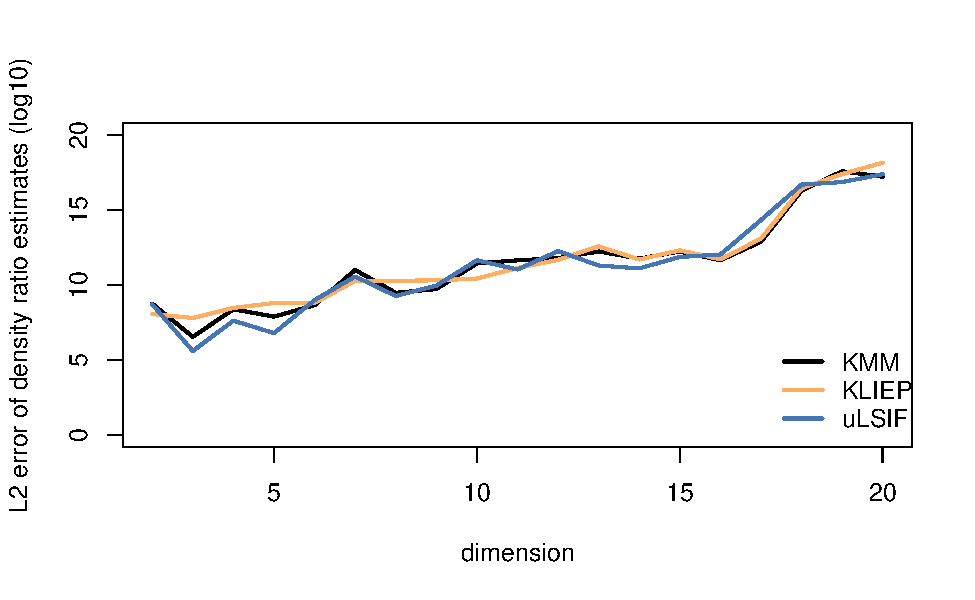
\includegraphics{l2_density_ratio.pdf}
    \caption{$\|\beta-\hat{\beta}\|^{2}$ for KMM, KLIEP and uLSIF against dimensionality of variables. The squared errors of density ratio are shown on log10 scale.}
    \label{l2_density_ratio.pdf}
\end{figure}

Additionally, for each dimension, we fit a weighted logistic regression on the training samples, then use it to predict the labels of the test samples. We use the area under the ROC curve (AUC) as the evaluation metric.
\begin{table}[H]
	\centering
\begin{tabular} {c | c | c | c }
dimensionality & KMM & KLIEP & uLSIF  \\
\hline \hline
2 & 0.514 (0.081) & 0.513 (0.093) & 0.511 (0.090)  \\
5 & 0.501 (0.103) & 0.502 (0.105) & 0.510 (0.112) \\
8 & 0.471 (0.100) & 0.477 (0.106) & 0.478 (0.102) \\
11 & 0.499 (0.112) & 0.507 (0.105) & 0.504 (0.109) \\
14 & 0.479 (0.136) & 0.496 (0.110) & 0.500 (0.113) \\
17 & 0.492 (0.107) & 0.472 (0.121) & 0.477 (0.119) \\
20 & 0.485 (0.108) & 0.494 (0.108) & 0.489 (0.101) \\
\hline \hline
\end{tabular}	
\caption{Average AUC for different density ratio estimation methods over a range of feature dimensionality, values in bracket indicates the standard deviation.}
\label{tab_sim}
\end{table}

Table \ref{tab_sim} shows that the AUC decreases and its standard deviation increases as the dimensionality of the variables grows. This illustrates that when using these density ratio estimation algorithms on datasets with high dimensions, the predictive performance worsens and the prediction risk in the test domain increases. This motivates the next chapter: by first reducing the feature dimensionality, the performance of these algorithms may be enhanced.



\pagebreak
%
%
%
%=============================================================
% Supervised Dimension Reduction
%=============================================================
%
%
%
\section{Supervised Dimension Reduction} \label{Supervised Dimension Reduction}
In genotype data modelling, dimension reduction is a standard processing step for a number of reasons. As mentioned above, a lower dimensional feature representation may lead to improved accuracy on density ratio estimates and lower test domain prediction risk. Genotype data are characterised by an enormous number of variants with a complex correlation structure. Such a large number of variables can cause issues such as singularity and can result some algorithms being unable to perform. [\cite{wang2011dimension}]. Performance of predictive models depends on the interrelationship between model complexity, sample size and feature dimension, sophisticated models with high dimensional feature space but moderate sample size can severely overfit. In statistical learning, a rule of thumb is to have at least 10 samples for each feature dimension [\cite{jain2000statistical}]. However, in gene expression data, this ratio is very small. For example, for the UK Biobank dataset studied in this report (see chapter \ref{biodata}), the ratio is around 0.51. This weakens the validity of predictive results and can easily generate false positives [\cite{wang2008approaches}]. Further, the amount of computation required increases with the dimensionality of features. Hence, finding a lower dimensional feature representation can reduce both time complexity and space complexity when implement algorithms. It is worth noting that in genotype data, unsupervised dimension reduction methods are often ineffective because they do not account for the relevance of the features to the target labels. For example, in unsupervised PCA, a smaller dimensional features are constructed as a linear combination of genotypes in the original dataset, this approach assumes the direction with majority of variation contains the majority of information. However, this is always not true in genotype datasets where a phenotype is only affected by a small subset of genotypes, using such unsupervised methods may cause informative genes with weaker signals to be left out. Thus, investigating useful supervised dimension reduction (SDR) techniques will be our main focus. 

There are multiple ways of to perform SDR in the context of genotype data. One approach is to select a small subset of genotypes based on a specific univariate measurement. This method is easy to understand, perform and interpret. It is often easily scalable to the dimensionality of the data. However, relies on the unrealistic assumption that the genotypes are independent to each other. Therefore, the results can carry a lot of noise and the selected genotypes are often highly correlated, which can create problems in subsequent analysis [\cite{wang2011dimension}]. Alternatively, we can construct features as a linear or non-linear combination of genotypes, which better takes the correlation structure into consideration. In this chapter, we will introduce a few of such SDR methods, followed by a discussion about their strengths and limitations. 
%
%
%
%=============================================================
% Supervised PCA
%=============================================================
%
%
%

\subsection{Supervised PCA} \label{Supervised PCA}
Unlike traditional PCA methods that create new uncorrelated variables by successively maximising the variance, the supervised PCA (SPCA)  [\cite{barshan2011supervised}], estimates a sequence of principal components that have maximal dependence on the labels, thus giving more effective information fr the subsequent prediction tasks. The detailed mathematical framework for this algorithms is described as follows:

\subsubsection{Hilbert-Schmidt Independence Criterion (HSIC)}  
To quantify the dependence between two random variables, say, $\boldsymbol{X}$ and $\boldsymbol{Y}$, we use the Hilbert-Schmidt Independence Criterion (HSIC) [\cite{gretton2005measuring}]. The HSIC is based on the fact that $\boldsymbol{X}$ and $\boldsymbol{Y}$ are independent if and only if any continuous bounded function of these two variables are uncorrelated. 

Specifically, given observations $\left\{\left(x_{1}, y_{1}\right), \ldots,\left(x_{n}, y_{n}\right)\right\} \sim P_{XY}$, we test their dependence against the null hypothesis $P_{XY} = P_{X} \times P_{Y}$. Let $\mathcal{H}$ be a Hilbert space of functions $f: \mathcal{X} \rightarrow \mathbb{R}$ defined on a non-empty set $\mathcal{X}$. A function $k: \mathcal{X} \times \mathcal{X} \rightarrow \mathbb{R}$ is called a reproducing kernel of $\mathcal{H}$ if it satisfies

(1) $\forall x \in \mathcal{X}, \quad k_{x}=k(\cdot, x) \in \mathcal{H}$ \\
(2) $\forall x \in \mathcal{X}, \forall f \in \mathcal{H},\langle f, k(\cdot, x)\rangle_{\mathcal{H}}=f(x)$ (the reproducing property).

If $\mathcal{H}$ has a reproducing kernel, it is called a reproducing kernel Hilbert space (RKHS). Define $\mathcal{F}$ as a separable RKHS that contains all continuous bounded real value functions of $x \in \mathcal{X}$ to $\mathbb{R}$. Let the linear product in the kernel space be given by $k(\cdot,\cdot)$. Similarly define $\mathcal{G}$ as the RKHS of $y \in \mathcal{Y}$ to $\mathbb{R}$ with kernel function $l(\cdot,\cdot)$. Denote the covariance operator that maps elements of $\mathcal{G}$ to the elements of $\mathcal{F}$ as $C_{x, y}: \mathcal{G} \rightarrow \mathcal{F}$. Then the cross-covariance between elements of  $\mathcal{F}$ and  $\mathcal{G}$ is 
\begin{equation*}
\left\langle f, C_{x y} g\right\rangle=\operatorname{Cov}(f(x), g(y))=\mathbb{E}_{x, y}[f(x), g(y)]-\mathbb{E}_{x}[f(x)] \mathbb{E}_{y}[g(y)] \hspace{15pt} \forall f \in \mathcal{F}, \forall g \in \mathcal{G} \text{.}
\end{equation*}
From the reproducing property of RKHS, we know that $f(x) = \langle f, k(\cdot, x)\rangle_{\mathcal{F}}$ and $g(y) = \langle f, k(\cdot, x)\rangle_{\mathcal{G}}$. Then this covariate operator can be expressed as
\begin{equation*}
C_{x y}=\mathbb{E}_{x, y}[k(x, \cdot) l(y, \cdot)]-\mathrm{E}_{x}[k(x, \cdot)] \mathbb{E}_{y}[l(y, \cdot)]   \hspace{15pt}\text{.}
\end{equation*}
The dependence between $\boldsymbol{X}$ and $\boldsymbol{Y}$ is measured by the HSIC which is defined as the square of the Hilbert-Schmidt (HS) norm of the cross-covariance operator $C_{x y}$. The HS norm is defined as follows:
\begin{equation*}
\|C_{x y}\|_{H S}^{2}:=\sum_{i, j}\left\langle C v_{i}, u_{j}\right\rangle_{\mathcal{F}}^{2}
\end{equation*}
where $u_{j}$ and $v_{i}$ are orthogonal bases of $\mathcal{F}$ and $\mathcal{G},$ respectively. The HSIC can be further expressed in terms of kernel functions:

\begin{align*}
H S I C\left(P_{XY}, \mathcal{F}, \mathcal{G}\right)&:=\left\|C_{x y}\right\|_{HS}^{2} \\
&=\mathrm{E}_{x, x^{\prime}, y, y^{\prime}}\left[k\left(x, x^{\prime}\right) l\left(y, y^{\prime}\right)\right]+\mathrm{E}_{x, x^{\prime}}\left[k\left(x, x^{\prime}\right)\right] \mathrm{E}_{y, y^{\prime}}\left[l\left(y, y^{\prime}\right)\right] \\
& -2 \mathrm{E}_{x, y}\left[\mathrm{E}_{x^{\prime}}\left[k\left(x, x^{\prime}\right)\right] \mathrm{E}_{y^{\prime}}\left[l\left(y, y^{\prime}\right)\right]\right] 
\end{align*}

where $\mathbf{E}_{x, x^{\prime}, y, y^{\prime}}$ denotes the expectation over independent pairs of $(x, y)$ and $\left(x^{\prime}, y^{\prime}\right)$ drawn from $P_{\boldsymbol{X}, \boldsymbol{Y}}$. As long as $k,l$ are universal kernels, $\|C_{x y}\|_{H S}^{2} = 0$ if and only if $\boldsymbol{X}$ and $\boldsymbol{Y}$ are independent.

In practice, the empirical HSIC used as an approximation to the test statistic:
\begin{equation} \label{HSIC equation}
\widehat{HSIC}=\frac{1}{(n-1)^{2}} \operatorname{tr}(KHLH)
\end{equation} 
where $H, K, L \in \mathbb{R}^{n \times n}$, $K_{i j}:=k\left(\mathbf{x}_{i}, \mathbf{x}_{j}\right)$, $L_{i j}:=l\left(\mathbf{y}_{i}, \mathbf{y}_{j}\right)$, and H is the centering matrix defined as $H_{i j}:=I - n^{-1} \mathbf{e} \mathbf{e}^{T}$. From equation \ref{HSIC equation} we conclude that to maximise the dependence between two kernels, we need to maximise the trace of $(K H L H)$

\subsubsection{Supervised PCA Algorithm} 
Suppose our dataset consists of $n$ samples and each sample has $p$ features, then the feature matrix $X$ has dimension $p \times n$. Further denote $Y_{\ell \times n}$ a matrix of outcome measures, where $\ell$ indicates the number of classes of labels. The goal is to map $X$ to a lower dimensional subspace $U^{T}X$ such that the dependence between the projected data points $U^{T}X$ and $Y$ is maximised. Substitute $K$ with the kernel of $U^{T}X$ and $L$ with the kernel of $Y$ into equation \ref{HSIC equation} (here we assume both kernels are linear for simplicity, but in practice it can be chosen depending on the characteristics of the dataset), we obtain:
\begin{align*}
\operatorname{tr}(H K H L) & =\operatorname{tr}\left(H X^{T} U U^{T} X H L\right) \\
& =\operatorname{tr}\left(U^{T} X H L H X^{T} U\right)
\end{align*}

We wish to find an orthogonal transformation matrix $U$ such that the features in the subspace uncorrelated. To achieve this, we add the following constraint:
\begin{equation} \label{SPCA}
\begin{array}{cc}\arg \max _{U} & \operatorname{tr}\left(U^{T} X H L H X^{T} U\right) \\
\text {subject to} & U^{T} U=I
\end{array}
\end{equation}
This formulation is similar to the optimisation problem for traditional PCA and it is clear that the the solution can be obtained via eigendecomposition of the real and symmetric matrix $Q = X H L H X^{T}$. Suppose $Q$ has the following $p$ eigenvalues $\lambda_{1} \geq \ldots \geq \lambda_{p}$, corresponding to eigenvectors $v_{1}, \ldots, v_{p}$. To obtain a subspace in $\mathbb{R}^{d}$ where $d \ll p$, the solution is $U=\left[v_{1}, v_{2}, \ldots, v_{d}\right]$. Note that when the kernel matrix $L$ is equivalent to an identity matrix $I$, the supervised PCA reduces to the unsupervised case. 

\subsubsection{The Dual Problem} 
The above solution of SPCA can also be derived by solving its dual optimisation problem, meaning that the eigendecomposition is to perform on an $n \times n$ matrix, rather than a $p \times p$ matrix. The dual problem is more computationally efficient for our dataset since the number of genotypes far exceed the sample size. 

The matrix $Q$ and the kernel matrix $L$ in the primal problem are positive semi-definite and hence can be decomposed as follows:
\begin{align*}
Q &=X H L H X^{T}=\Psi \Psi^{T}  \hspace{20pt} \Rightarrow \Psi =X H \Delta^{T}\\
L &=\Delta^{T} \Delta \\
\end{align*}
We can then apply the singular value decomposition (SVD) on $\Psi$ and rewrite $Q$ using the results of the SVD
\begin{align*}
\Psi &= U \Sigma V^{T} \\
Q &= U \Sigma \Sigma^{T} U^{T}
\end{align*}
It is evident that $U$ in the SVD consist of the eigenvectors of $Q$ and therefore, $U = \Psi V \Sigma^{-1}$ is the solution to the optimisation problem. To map $X$ to a $d$ dimensional subspace, we select first $d$ columns of matrix $U$, denoted as $\hat{U}_{p \times d}$, then the projected matrix is $\hat{U}^{T}X$. The pseudo-code for this algorithm is given as follows:

\begin{algorithm}[H]
\SetAlgoLined
 \KwInput{training feature matrix X, test data example x, kernel matrix of labels L, training data size n.}
 \KwOutput{Dimension reduced training data $\mathbf{Z}$ and test data $\mathbf{z}$.}
 Decompose $L$ such that $L=\Delta^{T} \Delta$.\\
 $H \leftarrow I-n^{-1} \mathbf{e e}^{T}$\\
 $\Psi \leftarrow X H \Delta^{T}$\\
 Compute basis:
 $\begin{array}{l}
 V \leftarrow \text { eigenvectors of } \Psi^{T} \Psi=\Delta H\left[X^{T} X\right] H \Delta^{T} \text { corresponding to the top } d \text { eigenvalues. } \\ 
 \qquad \begin{array}{l}\Sigma \leftarrow \text { diagonal matrix of square roots of the top } d \text { eigenvalues of } \Psi^{T} \Psi . \\ 
U \leftarrow \Psi V \Sigma^{-1}\end{array}\end{array}$\\
 Encode training data: $Z \leftarrow U^{T} X=\Sigma^{-1} V^{T} \Delta H\left[X^{T} X\right]$\\
 Encode test example: $\mathbf{z} \leftarrow U^{T} \mathbf{x}=\Sigma^{-1} V^{T} \Delta H\left[X^{T} \mathbf{x}\right]$\\
\caption{Dual Supervised PCA}
\end{algorithm}
Note that solving this optimisation problem does not involve expensive iterative optimisation procedures, making it suitable for high dimensional datasets.

\subsubsection{Kernel Supervised PCA}
Supervised PCA only allows linear combination of features, which may not always be effective. Here we extend the supervised PCA to allow nonlinear combinations by mapping the features onto a kernel space [\cite{ghojogh2019unsupervised}]. Define a feature map $\Phi$ which maps $x$ to a feature space $\mathcal{H}$ such that $\Phi: x \rightarrow \mathcal{H} $ and $x \mapsto \Phi(x)$. Also the kernel matrix of our dataset is $ {K}_{x}:= {K}( {X},  {X})= {\Phi}( {X})$. Then the Kernel Supervised PCA (KSPCA) can be formulated as:
\begin{equation*}
\arg \max _{U} \operatorname{tr}\left(U^{T} \Phi(X) H L H \Phi(X)^{T} U\right) \\
\text {subject to} \quad U^{T} U=I
\end{equation*}

As above, we let $Q = \Phi(X) H L H \Phi(X)^{T}$ and apply matrix decomposition on $Q$ and $L$ such that $Q = \Psi \Psi^{T}$ and $L=\Delta^{T} \Delta$. Then we perform SVD on $\Psi$ and obtain $\Psi = \Phi(X) H \Delta^{T} = U \Sigma V^{T}$ , where $U$ consists of the eigenvectors of $\Psi(X) \Psi(X)^{T}$. In practice, it is often difficult and unnecessary to compute the value of ${\Phi}({X})$ explicitly, especially it can be up to an infinite order. Instead, we use the the kernel matrix ${K}_{x}={K}({X}, {X})={\Phi}({X})^{\top} {\Phi}({X})$. Also, note that ${K}_{x}$ is an $n \times n$ matrix, so kSPCA is computationally feasible for datasets which have a relatively small number of samples but large number of features. By the representation theorem [\cite{fulton2013representation}], any solution $\boldsymbol{u} \in \mathcal{H}$ must lie in the span of the of all the training vectors mapped to the Hilbert space $\mathcal{H}$. Thus we can rewrite the transformation matrix $U$ as a linear projection of the projected data points, i.e. $U =\Phi(X) \beta$, where $\beta:=\left[\beta_{1}, \ldots, \beta_{p}\right] \in \mathbb{R}^{n \times p}$. Then the optimisation problem can be expressed as:
\begin{align*}
& \arg \max _{U} \operatorname{tr}\left(U^{T} \Phi(X) H L H \Phi(X)^{T} U\right) \\
& = \arg \max _{U}  \operatorname{tr}\left(\beta^{T} \Phi(X)^{T} \Phi(X) H L H \Phi(X)^{T} \Phi(X) \beta\right) \\
& = \arg \max _{U} \operatorname{tr}\left(\beta^{T} {K}_{x}HLH{K}_{x} \beta\right) \\
& \text {subject to} \quad U^{T} U = \beta^{T} {\Phi}({X})^{\top} {\Phi}({X}) \beta = \beta^{T} {K}_{x} \beta
\end{align*}
This is a generalised eigenvalue problem of $({K}_{x}HLH{K}_{x}, {K}_{x})$ and has a closed-form solution [\cite{ghojogh2019eigenvalue}]. Further, [\cite{ghojogh2019unsupervised}] shows that this optimisation problem can be alternatively solved by performing the eigendecomposition on $HLH{K}_{x}$.

The algorithm is illustrated using the following pseudo-code:

\begin{algorithm}[H]
\SetAlgoLined
 \KwInput{Kernel matrix of training data ${K}_{x}$, kernel matrix of testing data ${K}_{\text {test}}$, kernel matrix of target variable ${L}$, testing data example ${x}$, training data size n}
 \KwOutput{Dimension reduced training data $\mathbf{Z}$ and testing data $\mathbf{z}$.}
 $H \leftarrow I-n^{-1}$ ee $^{T}$.\\
 $Q \leftarrow {K}_{x} H L H {K}_{x}$ \\ 
 Compute basis: $\beta \leftarrow$ generalized eigenvectors of $(\mathrm{Q}, \mathrm{K})$ corresponding to the top $d$ eigenvalues. \\
 Encode training data: $\mathbf{Z} \leftarrow \beta^{T}\left[\Phi(X)^{T} \Phi(X)\right]=\beta^{T} {K}_{x}$ \\
 Encode test example: $\mathbf{z} \leftarrow \beta^{T}\left[\Phi(X)^{T} \Phi(\mathbf{x})\right]=\beta^{T} K_{\text {test}}$ \\
\caption{Kernel Supervised PCA}
\end{algorithm}

%
%
%
%=============================================================
% LKFDA
%=============================================================
%
%
%
\subsection{Local Fisher Discriminant Analysis}
Supervised PCA produces a projection with maximal dependence on the response variable but does not consider local structure of the data. In a genotype dataset, there is often the presence of multimodality. For example, the genotypes exhibits a  clustering structure since the contiguous genotypes are likely to be correlated. Since numerous clusters can cause participants to have a particular disease, these structure may reveal valuable information. As an alternative to supervised PCA, here we introduce Local Fisher Discriminant Analysis (LFDA) which integrates the idea of both Fisher Linear Discriminant Analysis (FDA) and Local Preserving Projection (LPP) such that the local structure of the data points in the original feature space is preserved in the embedding space.

\subsubsection{Fisher Linear Discriminant Analysis}
FDA is one of commonly applied supervised dimension reduction methods [\cite{fisher1936use}]. It finds a linear combination of features that maximises the separation between classes while minimising the variance of variance within each class. Suppose we have $p$ dimensional samples $x_{i} \in \mathbb{R}^{p}(i=1,2, \ldots, n)$ and the associated class labels $y_{i} \in\{1,2, \ldots, c\}$ where $c$ is the total number of classes. Also suppose $n_{j}$ to be the number of samples in class $\ell$ such that $\sum_{\ell=1}^{c} n_{\ell}=n$.

Denote $S^{(w)}$ and $S^{(b)}$ be the within-class scatter matrix and between-class scatter matrix respectively, which are defined as:
\begin{align} 
S^{(w)} & = \sum_{\ell=1}^{c} \sum_{i: y_{i}=\ell}\left(x_{i}-\mu_{\ell}\right)\left(x_{i}-\mu_{\ell}\right)^{\top} \label{sw}\\
S^{(b)} & = \sum_{\ell=1}^{c} n_{\ell}\left(\mu_{\ell}-\mu\right)\left(\mu_{\ell}-\mu\right)^{\top} \label{sb}
\end{align}
where $\mu_{\ell}$ is the mean of samples in class $\ell$, computed as $\mu_{\ell} = \frac{1}{n_{\ell}} \sum_{i: y_{i}=\ell} x_{i}$ and $\mu$ is the mean of all samples $\mu = \frac{1}{n} \sum_{i=1}^{n} x_{i}=\frac{1}{n} \sum_{\ell=1}^{c} n_{\ell} \mu_{\ell}$.

Assume that $S^{(w)}$ has full rank, then the FDA transformation matrix $T_{F D A}$ can be derived from solving the following optimisation problem:
\begin{equation*}
T_{F D A}=\underset{T \in \mathbb{R}^{p \times d}}{\operatorname{argmax}}\left[\frac{\operatorname{det}\left(T^{\top} S^{(b)} T\right)}{\operatorname{det}\left(T^{\top} S^{(w)} T\right)}\right]
\end{equation*}
where $d$ is the dimension of the projected feature space and $1 \leq d \leq p$. For this problem to be solvable, there is an implicit constraint that $\operatorname{rank}(T)=d$, otherwise the quantity in the denominator $T^{\top} S^{(w)} T$ is not invertible. The solution of the transformation matrix can be derived via solving the following generalised eigenvalue problem:
\begin{equation*}
S^{(b)} \varphi=\lambda S^{(w)} \varphi
\end{equation*}
where $\left\{\varphi_{k}\right\}_{k=1}^{p}$ are the generalised eigenvectors corresponding to the generalised eigenvalues $\lambda_{1} \geq \lambda_{2} \geq \cdots \geq \lambda_{p}$, then the transformation matrix $T_{F D A}$ is given as:
\begin{equation*}
T_{F D A}=\left(\varphi_{1}\left|\varphi_{2}\right| \cdots \mid \varphi_{d}\right)
\end{equation*}

\subsubsection{Local Preserving Projection (LPP)}
The Local Preserving Projection (LPP) is an unsupervised dimension reduction technique that preserves the local structure of the features after mapping [\cite{he2004locality}]. A brief introduction is given here.

Let $A$ be the $n \times n$ affinity matrix where $A_{i,j} \in [0,1]$ indicates the affinity between $x_{i}$ and $x_{j}$. $A_{i, j}$ is close to 1 if the distance between $x_{i}$ and $x_{j}$ is small, by contrast $A_{i, j}$ is close to 0 if the two samples are far apart. Some popular choice of the affinity matrix $A$ are (1) the heat kernel, which is expressed as $A_{i, j}=\exp \left(-\frac{\left\|x_{i}-x_{j}\right\|^{2}}{\sigma^{2}}\right)$ and $\sigma(>0)$ is a tunable decay parameter [\cite{belkin2003laplacian}]; (2) the nearest neighbour affinity[\cite{roweis2000nonlinear}] where we define $A_{i, j}=1$ if $x_{j}$ is the k-nearest neighbour of $x_{i}$ or vice verse and  $A_{i, j}=0$ if otherwise. In this paper, we illustrate the algorithm using local scaling, which takes into account that the density of samples may differ depending on their regions [\cite{zelnik2005self}]. The local scaling affinity matrix is defined as 
\begin{equation*}
A_{i, j}=\exp \left(-\frac{\left\|x_{i}-x_{j}\right\|^{2}}{\sigma_{i} \sigma_{j}}\right)
\end{equation*}
$\sigma_{i}$ indicates the local scaling of samples around $x_{i}$ computed as $\sigma_{i}=\left\|x_{i}-x_{i}^{(K)}\right\|$, where $x_{i}^{(K)}$ is the $K$-th nearest neighbour of $x_{i}$.

Then the LPP transformation matrix is defined as the following:
\begin{equation*}
T_{L P P} = \underset{T \in \mathbb{R}^{p \times d}}{\operatorname{argmin}}\left(\frac{1}{2} \sum_{i, j=1}^{n} A_{i, j}\left\|T^{\top} x_{i}-T^{\top} x_{j}\right\|^{2}\right) \\
\text { subject to } T^{\top} X D X^{\top} T=I_{d}
\end{equation*}

where $D$ is an $n \times n$ diagonal matrix with the $i$-th element on diagonal being $D_{i, i} = \sum_{j=1}^{n} A_{i, j}$. $D$ represents the local structure of the samples in the original space. The role of the constraint is to prevent degeneracy. The transformation matrix $T_{L P P}$ aims to keep data points which are close in the original space still close in the embedding space. This objective function can be further expressed as:
\begin{align*}
T_{L P P} & = \underset{T \in \mathbb{R}^{p \times d}}{\operatorname{argmin}}\left(\frac{1}{2} \sum_{i, j=1}^{n} A_{i, j}\left\|T^{\top} x_{i}-T^{\top} x_{j}\right\|^{2}\right) \\
& =  \underset{T \in \mathbb{R}^{p \times d}}{\operatorname{argmin}} \left( T^{T}X(D-A)X^{T}T \right) \\
& = \underset{T \in \mathbb{R}^{p \times d}}{\operatorname{argmin}} \left( T^{T}XLX^{T}T \right)
\end{align*}
where $L = D - A$ is named the Laplacian matrix. We further denote $\left\{\psi_{k}\right\}_{k=1}^{p}$ as the generalised eigenvectors corresponding to the generalised eigenvalues $\gamma_{1} \geq$ $\gamma_{2} \geq \cdots \geq \gamma_{p}$ of the following generalised eigenvalue problem:
\begin{equation*}
X L X^{\top} \Psi=\gamma X D X^{\top} \Psi
\end{equation*}
As shown in [\cite{he2004locality}], the optimal solution is given by 
\begin{equation*}
T_{L P P}=\left(\Psi_{p}\left|\Psi_{p-1}\right| \cdots \mid \Psi_{p-d+1}\right)
\end{equation*}

\subsubsection{Local Fisher Discriminant Analysis (LFDA)}
LLP is an unsupervised method which ignores the connection between the features and the labels while LDA is supervised but ignores the local structure of the features. Here, we combine the two methods to construct the Local Fisher Discriminant Analysis (LFDA) algorithm. LFDA is formulated as follows [\cite{sugiyama2007dimensionality}].

First, we rewrite $S^{(w)}$ and $S^{(b)}$ in equation \ref{sw} and \ref{sb} as 
\begin{equation} \label{s}
\begin{array}{l}
S^{(w)}=\frac{1}{2} \sum_{i, j=1}^{n} W_{i, j}^{(w)}\left(x_{i}-x_{j}\right)\left(x_{i}-x_{j}\right)^{\top} \\
S^{(b)}=\frac{1}{2} \sum_{i, j=1}^{n} W_{i, j}^{(b)}\left(x_{i}-x_{j}\right)\left(x_{i}-x_{j}\right)^{\top}
\end{array}
\end{equation}
where 
\begin{equation} \label{w}
\begin{array}{l} 
W_{i, j}^{(w)} = \left\{\begin{array}{cl}
A_{i,j} / n_{\ell} & \text { if } y_{i}=y_{j}=\ell \\
0 & \text { if } y_{i} \neq y_{j}
\end{array}\right. \\
W_{i, j}^{(b)} = \left\{\begin{array}{cl}
A_{i,j} (1 / n-1 / n_{\ell}) & \text { if } y_{i}=y_{j}=\ell \\
1 / n & \text { if } y_{i} \neq y_{j}
\end{array}\right.
\end{array}
\end{equation}
The derivation is given below:

\begin{align*}
S^{(w)} &=\sum_{\ell=1}^{c} \sum_{i: y_{i}=\ell}\left(x_{i}-\frac{1}{n_{\ell}} \sum_{j: y_{j}=\ell} x_{j}\right)\left(x_{i}-\frac{1}{n_{\ell}} \sum_{j: y_{j}=\ell} x_{j}\right)^{\top} \\
&=\sum_{i=1}^{n} x_{i} x_{i}^{\top}-\sum_{\ell=1}^{c} \frac{1}{n_{\ell}} \sum_{i, j: y_{i}=y_{j}=\ell} x_{i} x_{j}^{\top} \\
&=\sum_{i=1}^{n}\left(\sum_{j=1}^{n} W_{i, j}^{(w)}\right) x_{i} x_{i}^{\top}-\sum_{i, j=1}^{n} W_{i, j}^{(w)} x_{i} x_{j}^{\top} \\
&=\frac{1}{2} \sum_{i, j=1}^{n} W_{i, j}^{(w)}\left(x_{i} x_{i}^{\top}+x_{j} x_{j}^{\top}-x_{i} x_{j}^{\top}-x_{j} x_{i}^{\top}\right)
\end{align*}

Additionally, define $S^{(m)}$ as the mixture scatter matrix [\cite{fukunaga2013introduction}] where $S^{(m)} = S^{(w)}+S^{(b)} =\sum_{i=1}^{n}\left(x_{i}-\mu\right)\left(x_{i}-\mu\right)^{\top}$, then we obtain

\begin{align*}
S^{(b)} &=\sum_{i=1}^{n} x_{i} x_{i}^{\top}-\frac{1}{n} \sum_{i, j=1}^{n} x_{i} x_{j}^{\top}-S^{(w)} \\
&=\sum_{i=1}^{n}\left(\sum_{j=1}^{n} \frac{1}{n}\right) x_{i} x_{i}^{\top}-\sum_{i, j=1}^{n} \frac{1}{n} x_{i} x_{j}^{\top}-S^{(w)} \\
&=\frac{1}{2} \sum_{i}^{n}\left(\frac{1}{n}-W_{i, j}^{(w)}\right)\left(x_{i} x_{i}^{\top}+x_{j} x_{j}^{\top}-x_{i} x_{j}^{\top}-x_{j} x_{i}^{\top}\right)
\end{align*}

as required.

Notice that in equation \ref{w}, the affinity matrix $A$ is defined such that $A_{i,j}$ is large only for data points $x_{i}$ and $x_{j}$ that are not far apart. Hence, when $x_{i}$ and $x_{j}$ are in the same class and they are close to each other, $W_{i, j}^{(w)}$ is positive while $W_{i, j}^{(b)}$ is negative, implying that the within-class scatter becomes small and the between-class scatter becomes large. By contrast, when $x_{i}$ and $x_{j}$ are in different classes, their within-class scatter shrinks and the between-class scatter increases. 

We further define the LFDA transformation matrix $T_{L F D A}$ as
\begin{equation*}
T_{L F D A}=\operatorname{argmax}_{T \in \mathbb{R}^{p \times d}}\left[\operatorname{tr}\left(\left(T^{T} S^{(w)} t\right)^{-1} T^{T} S^{(b)} T\right)\right]
\end{equation*}
This can be solved by finding the generalised eigenvalues and generalised eigenvectors $\left\{{\lambda}_{k}, {\varphi}_{k}\right\}_{k=1}^{r}$ of the following generalised eigenvalues problem:
\begin{equation} \label{lfda}
{S}^{(b)} {\varphi}={\lambda} {S}^{(w)} {\varphi}
\end{equation}
The optimal LDFA transformation matrix is given by
\begin{equation*}
T_{L F D A}=\left(\sqrt{{\lambda}_{1}} {\varphi}_{1}\mid\sqrt{{\lambda}_{2}} {\varphi}_{2}\mid \cdots\mid\sqrt{{\lambda}}_{d} {\varphi}_{d}\right)
\end{equation*}
where ${\lambda}_{1} \geq {\lambda}_{2} \geq \cdots \geq {\lambda}_{p}$.

The algorithm is demonstrated in terms of pseudo-code, shown in the below:

\begin{algorithm}[H]
\SetAlgoLined
 \KwInput{feature matrix of training data, $X_{p \times n}$, training data labels $Y$, dimensionality of reduced space, $d$ , number of neighbours to account for in KNN, k}
 \KwOutput{$d \times r$ transformation matrix $T_{L F D A}$.}
 ${S}^{(b)} \longleftarrow 0_{p \times p}$ \tcp*{$0_{p \times p}$ denotes the $p \times p$ matrix of zeroes }
 ${S}^{(w)} \longleftarrow 0_{p \times p}$ \; 
 \For{$\ell=1,2, \ldots, c$ \tcp*{compute the scatter matrix for each class}} {
 $\left\{\underline{x}_{i}\right\}_{i=1}^{n_{\ell}} \longleftarrow\left\{x_{j}\right\}_{j: y_{j}=\ell}$ \;
 \For{$i=1,2, \ldots, n_{\ell}$ \tcp*{determine local scaling}}{ 
 $\underline{x}_{i}^{(k)} \longleftarrow k$th nearest neighbor of $\underline{x}_{i}$ among $\left\{\underline{x}_{j}\right\}_{j=1}^{n_{\ell}}$ \;
 $\underline{\sigma}_{i} \longleftarrow\left\|x_{i}-\underline{x}_{i}^{(k)}\right\|$ }
 \For{$i, j=1,2, \ldots, n_{\ell} $ \tcp*{define the affinity matrix}} {
 $\underline{A_{i, j}} \longleftarrow \exp \left(-\left\|\underline{x}_{i}-\underline{x}_{j}\right\|^{2} /\left(\underline{\sigma}_{i} \underline{\sigma}_{j}\right)\right)$}
 $\underline{X} \longleftarrow\left(\underline{x}_{1}\left|\underline{x}_{2}\right| \cdots \mid \underline{x}_{n_{\ell}}\right)$ \;
 $\underline{G} \longleftarrow \underline{X} \operatorname{diag}\left(\underline{A}{1}_{n_{\ell}}\right) \underline{X}^{\top}-\underline{X} \underline{A} \underline{X}^{\top}$ \;
 $S^{(b)} \longleftarrow {S}^{(b)}+\underline{G} / n+\left(1-n_{\ell} / n\right) \underline{X} \underline{X}^{\top}+\underline{X} 1_{n_{\ell}}\left(\underline{X} 1_{n_{\ell}}\right)^{\top} / n$ \;
 $S^{(w)} \longleftarrow {S}^{(w)}+\underline{G} / n_{\ell}$}
 $S^{(b)} \longleftarrow S^{(b)}-X 1_{n}\left(X 1_{n}\right)^{\top} / n- S^{(w)}$ \;
 $\left\{\lambda_{k}, \varphi_{k}\right\}_{k=1}^{r} \longleftarrow$ generalized eigenvalues and normalized eigenvectors of $\varphi=\lambda S^{(w)} \varphi ; \quad \% \lambda_{1} \geq \lambda_{2} \geq \cdots \geq \lambda_{d}$ \;
$T_{L F D A}=\left(\sqrt{\lambda_{1}} {\varphi}_{1}\left|\sqrt{{\lambda}}_{2}{\varphi}_{2}\right| \cdots \mid \sqrt{{\lambda}_{r}} {\varphi}_{r}\right)$
\caption{Local Linear Fisher Discriminant Analysis}
\end{algorithm}

Notice that based on this formulation, two data points that are in the same class but far from each other do not come closer in the embedding space. One major advantage of LFDA over traditional FDA is that in the latter, the between-class scatter matrix $S^{(b)}$ has at most rank $c-1$, implying that it can find at most $c-1$ dimensions of meaningful features while the remaining dimensions resulted from FDA are merely arbitrary [\cite{fukunaga2013introduction}]. This limitation makes FDA ineffective for the UK Biobank dataset we used on this report where the genotypes have only two classes and reducing a $\sim780,000$ dimensional feature space to a one dimensional space is clearly not sensible. In contrast, the local between-class scatter matrix from LFDA in general has much higher rank because we incorporat the affinity matrix $A$ into the weights. Thus, the LFDA can be practically implemented for dimensionality reduction into any dimensional space.

\subsubsection{Kernel Local Linear Fisher Discriminant Analysis (KLFDA)}
Similar as SPCA, LFDA can be kernelised to allow non-linear dimension reduction. Also, by using the kernel trick, the computational burden is greatly eased since the dimension of the kernel matrix is only decided by the sample size, not the dimensionality of features. To illustrate this algorithm, we will start with the LFDA optimisation problem we described previously, then show that it is possible to incorporate kernel methods into its formulation.

Recall that in LFDA (equation \ref{lfda}), the transformation matrix is solved by:
\begin{equation*} 
{S}^{(b)} {\varphi}={\lambda} {S}^{(w)} {\varphi}
\end{equation*}
Also previously we have defined ${S}^{(m)}$ as the local mixture scatter matrix which is the sum of between-class and within-class scatters, i.e. ${S}^{(m)} = {S}^{(b)}+{S}^{(w)}$. From equation \ref{s} and \ref{w}, ${S}^{(m)}$ can be expressed as [\cite{sugiyama2007dimensionality}]:
\begin{align} \label{eq}
{S}^{(m)} &= \frac{1}{2} \sum_{i, j=1}^{n} {W}_{i, j}^{(m)}\left(x_{i}-x_{j}\right)\left(x_{i}-x_{j}\right)^{\top} \\
&=\frac{1}{2} \sum_{i, j=1}^{n} {W}_{i, j}^{(m)}\left(x_{i} x_{i}^{\top}+x_{j} x_{j}^{\top}-x_{i} x_{j}^{\top}-x_{j} x_{i}^{\top}\right) \\
&=\sum_{i=1}^{n}\left(\sum_{j=1}^{n} {W}_{i, j}^{(m)}\right) x_{i} x_{i}^{\top}-\sum_{i, j=1}^{n} {W}_{i, j}^{(m)} x_{i} x_{j}^{\top}
\end{align}
where $W^{(m)} = W^{(s)} + W{(b)}$ and is expressed as
\begin{equation*}
{W}_{i, j}^{(m)} = \left\{\begin{array}{cc}
A_{i, j} / n & \text { if } y_{i}=y_{j} \\
1 / n & \text { if } y_{i} \neq y_{j}
\end{array}\right.
\end{equation*}
We can further write equation \ref{eq} using its matrix form:
\begin{equation*}
{S}^{(m)}=X {L}^{(m)} X^{\top}
\end{equation*}
where 
\begin{equation*}
{L}^{(m)} = {D}^{(m)}-{W}^{(m)}
\end{equation*}
 and $D^{(m)}$ is an $n \times n$ diagonal matrix with its $i$th diagonal element being 
 \begin{equation*}
{D}_{i, i}^{(m)} = \sum_{j=1}^{n} {W}_{i, j}^{(m)} \hspace{50pt} \text{.}
\end{equation*}
Similarly, ${S}^{(w)}$ can be written as ${S}^{(w)}=X {L}^{(w)} X^{\top}$ where ${L}^{(w)} = {D}^{(w)}-{W}^{(w)}$ and ${D}_{i, i}^{(w)} = \sum_{j=1}^{n} {W}_{i, j}^{(w)}$. 

Then the LFDA problem (equation \ref{lfda}) can be written as:
\begin{equation} \label{klfda}
X {L}^{(b)} X^{\top} {\varphi}={\lambda} X {L}^{(w)} X^{\top} {\varphi}
\end{equation}
where ${L}^{(b)}={L}^{(m)}-{L}^{(w)}$. 

We can further express $X^{\top} {\varphi}$ in terms of a vector ${\alpha} \in \mathbb{R}^{n}$ such that
\begin{equation*}
X^{\top} {\varphi}=X^{\top} X {\alpha}=K \widetilde{\alpha}
\end{equation*}
where $K$ is an $n \times n$ kernel matrix with its element being $K_{i, j} \equiv x_{i}^{\top} x_{j}$. Then multiply both sides of equation \ref{klfda} by $X^{T}$, we have 
\begin{equation} \label{klfda_h}
K {L}^{(b)} K {\alpha}={\lambda} K {L}^{(w)} K {\alpha}
\end{equation}
This shows that $\left\{x_{i}\right\}_{i=1}^{n}$ only appears in the form of its linear product, thus we can consider any non-linear mapping $\phi(\cdot)$ on $x$ from the original feature space to a RKHS $\mathcal{H}$, then the matrix $K$ in equation \ref{klfda_h} represents the corresponding reproducing kernel matrix. Note that $K {L}^{(w)} K$ is always degenerate, leading the generalised eigenvalues problem to be unsolvable [\cite{sugiyama2007dimensionality}], so it is necessary to regularise $K {L}^{(w)} K$. One possible means of regularisation adds a small constant $\varepsilon$ and solves the following problem [\cite{friedman1989regularized}]:
\begin{equation*}
K {L}^{(b)} K {\alpha}={\lambda}\left(K {L}^{(w)} K+\varepsilon I_{n}\right) {\alpha}
\end{equation*}
This gives the optimal transformation matrix of KLFDA as:
 \begin{equation*}
\left(\sqrt{{\lambda}_{1}} {\alpha}_{1}\mid\sqrt{{\lambda}_{2}} {\alpha}_{2}\ \cdots \mid \sqrt{{\lambda}}_{r} {\alpha}_{r}\right)^{\top}\left(\begin{array}{c}
K\left(x_{1}, x^{\prime}\right) \\
K\left(x_{2}, x^{\prime}\right) \\
\vdots \\
K\left(x_{n}, x^{\prime}\right)
\end{array}\right)
\end{equation*}
%
%
%
%=============================================================
% NMF
%=============================================================
%
%
%
%
\subsection{Supervised Non-negative Matrix Factorisation}
In our data, an element $X_{ij}$ of the feature matrix is, in fact, the number of copies of the most frequent minor allele of the $i$th SNP for the $j$th person (note that the dimension of $X$ is $p \times n$), which only takes values 0,1 or 2. In other words, each element in the feature matrix is either zero or positive, making $X$ a non-negative matrix. In this case, Non-negative Matrix Factorisation (NMF) can be employed for dimension reduction and we can further make this algorithm supervised such that the features in the reduced dimension are more useful in discriminating different labels.

\subsubsection{The NMF Model}
The main idea of NMF is to approximate a non-negative matrix $X$ by the product of two non-negative matrices $T$ and $W$ [\cite{lee1999learning}], i.e.
\begin{equation*}
X_{p \times n} \approx T_{p \times k} W_{k \times n}
\end{equation*}
where $T$ is referred to the type matrix and $W$ is the weight matrix. The weight matrix consists of the coefficients by which the features of each sample can be constructed as a linear combination of columns (subcommunities) of the type matrix. The rank $k$ of this approximation is chosen in a way that $(p+n)k \ll n p$, and thus the dimension is reduced significantly. Also, $k$ is a parameter that determines the complexity of the model and needs to be tuned carefully. 

The implementation of NMF uses an iterative approach:
\begin{equation*}
\begin{array}{l}
T_{i a} \leftarrow T_{i a} \sum_{j} \frac{X_{i j}}{(T W)_{i j}} W_{a j} \\
T_{i a} \leftarrow \frac{T_{i a}}{\sum_{j} T_{j a}}\\
\hspace{25pt} \text{and} \\
W_{a j} \leftarrow W_{a j} \sum_{i} T_{i a} \frac{X_{i j}}{(TW)_{i j}}
\end{array}
\end{equation*}
These iterations converges to a local maximum of the following objective function [\cite{lee1999learning}]:
\begin{equation} \label{loglik}
L(T,W)=\sum_{i=1}^{p} \sum_{j=1}^{n}\left[X_{i j} \log (T W)_{i j}-(T W)_{i j}\right]
\end{equation}
subject to all elements in $X$, $T$ and $W$ are non-negative. We can interpret this objective function in terms of the likelihood where element of the feature matrix $X_{ij}$ is modelled as an independent Poisson observation given its mean $(TW)_{ij}$, then we are trying to maximise the likelihood of generating the features in $X$ from the type matrix $T$ and the weights $W$. In our dataset, notice that the consecutive genotypes may have high correlation and this covariance structure is implicitly given in the type matrix $T$. We further add constraints to $T$ such that each column sums to 1. Then each column can be interpreted as the composition of genotypes for each subcommunity. The general structure of NMF is illustrated using the pseudo code as the following:

\begin{algorithm}[H]
\SetAlgoLined
 \KwInput{feature matrix of training data $X_{p \times n}$, number of features in the reduced space $k \ll min[p,n]$}
 \KwOutput{a $p \times k$ type matrix $T$ and a $k \times n$ weight matrix $W$.}
 $T \longleftarrow 0_{p \times k}$ \;
 $W \longleftarrow 0_{k \times n}$ \tcp*{Initialise matrix $T$ and matrix $W$.} 
 \For{$i=1,2, \ldots, maxIter$}{
$T_{i a} \leftarrow T_{i a} \sum_{j} \frac{X_{i j}}{(T W)_{i j}} W_{a j}$ \;
$T_{i a} \leftarrow \frac{T_{i a}}{\sum_{j} T_{j a}}$ \;
$W_{a j} \leftarrow W_{a j} \sum_{i} T_{i a} \frac{X_{i j}}{(TW)_{i j}}$ \;
check the stopping criterion\
\tcp*{the stopping criterion can be the KL divergence $D(X\|T W)$ is within some threshold} 
}
return $T, W$
\caption{Non-negative matrix factorisation}
\end{algorithm}

\subsubsection{Supervised NMF (SNMF)}
The supervised version of NMF [\cite{cai2017learning}] performs NMF on each class separately at first then combine the results into a single type matrix, such that each sample can be expressed as a mixture of all subcommunities. Suppose feature $X$ are from $c$ classes:
\begin{equation*}
X=\left(X^{(1)}, X^{(2)}, \cdots, X^{(c)}\right)
\end{equation*}
where $X^{(i)}$ represents observations from the $i$th class. Then for each class, we obtain its corresponding type matrix $T^{(i)}$ via unsupervised NMF, then we combine these type matrices together to obtain a type matrix for all classes.
\begin{equation*}
T=\left(T^{(1)}, T^{(2)}, \cdots, T^{(c)}\right)
\end{equation*}
$T$ is still non-negative since each component $T^{(i)}$ is non-negative. Under the assumption that the rows of $W$ are independent for different samples, for a fixed $T$, maximising the total Poisson log likelihood is equivalent to maximising the Poisson log likelihood of each sample. Hence, we can consider $W$ as the non-negative coefficients for Poisson regression of $X$ on $T$ which maximise the Poisson log likelihood. For a sample $X_{j}=\left(X_{1 j}, X_{2 j}, \cdots, X_{p j}\right)$, we fit a regression on $T$ and make the resulting coefficients $W_{j}=\left(w_{1 j}, \cdots , w_{k j}\right)$ either zero (meaning the the corresponding variable in $T$ is removed from the regression) or positive. The elements of $W$ are computed via the following forward-backward procedure:

\begin{enumerate}
\item Fit a Poisson regression on $T$, assuming no intercept and identity link function. Also denote the coefficients of linear least square regression of $X_j$ on $T$ as initial values of $W_{j}$.  If any coefficients in $W_{j}$ are negative, remove the corresponding variables from the regression.
\item If any variables are removed, repeat step 1 until all the coefficients of the regression are positive. So far, the non-negativity constraints on $X$, $T$ and $W$ are satisfied. We denote this non-negative type matrix which has all coefficients non-negative as $T_{j}^{+}$, this is non-empty unless $X$ is a zero matrix.
\item Compute the log likelihood by using equation \ref{loglik}, i.e.
\begin{equation*}
L\left(T_{j}^{+}\right)=\sum_{i=1}^{p}\left(X_{i j} \log \left(T_{j}^{+} W_{j}\right)_{i}-\left(T_{j}^{+} W_{j}\right)_{i}\right)
\end{equation*}
\item For variables that are removed in Step 1 and Step 2, choose one and denote as $T_{j(new)}^{+}$, assign it to a very small positive coefficient that is denoted as $\epsilon$, then compute the log likelihood for the new set of variables:
\begin{equation*}
L\left(T_{j(new)}^{+}\right) =\sum_{i=1}^{p}\left(X_{i j} \log \left(T_{j(new)}^{+} W_{j(new)}\right)_{i}-\left(T_{j(new)}^{+} W_{j(new)}\right)_{i}\right)
\end{equation*}
where $W_{j(new)}=\left(W_{j}(1-\varepsilon), \varepsilon\right)$. Here, we need to rescale $W_{j}$ because we assume the data follow a Poisson distribution, so the sum of elements in $X_{j}$ should equal the sum of $TW_{j}$. We have add a constraint on the column sum of $T$ to be 1 previously, so we need $W_{j}^{T} 1=W_{j}^{T} T^{T} 1=X_{j}^{T} 1 = W_{j(new)}^{T} 1$, by defining $W_{j(new)}$ as above, we can ensure the sum of elements in $W_{j(new)}$ is the same as in $X_{j}$.
\item Compare $L\left(T_{j}^{+}\right)$ in step 3 and $L\left(T_{j(new)}^{+}\right)$ in Step 4 and if the latter is larger, i.e. by adding one more variable with non-negative coefficient $\epsilon$, the log likelihood is increased, we use the new type matrix $T_{j(new)}^{+}$ then repeat Step 1-5. Otherwise set $W_{j(new)}$ to zero again.
\item Repeat Step 4 and Step 5 for all the removed variables.
\end{enumerate}

Mote that the algorithm increases the log likelihood at each iteration, thus as long as the number of positive variables is finite, the convergence to maximum log likelihood is guaranteed. 

\subsubsection{Selecting the Number of Types}  \label{Choose The Number of Types}
For the supervised NMF algorithm, we need to select the number of types $k_{1} \cdots k_{c}$ for each class. These should be chosen in a way such that when we combine the individual type matrices together, the resulting matrix can most effectively discriminate these classes. A naive approach would be to attempt all combination of $k_{1} \cdots k_{c}$ (i.e. for class $i$, $k_{i}$ is chosen from $k_{i} = 1, \cdots, p$). Firstly, compute the combined type matrix $T$ and combined weight matrix $W$ on training samples for each combination. Then compare the model mis-classification errors on the validation set. However, this method is computationally expensive especially given the large number of genotypes $p$ in our dataset. To perform this approach, $p^{2}$ combinations need to be attempted.

Here, we use another algorithm, proposed in [\cite{cai2017learning}], which chooses the number of types for each class separately; then compares the deviances for each observation in the test set; followed by a Wilcoxon Rank-Sum test on these deviances; then standardise the test statistic for each fold and aggregate them into a single test statistic;  finally $k$ is chosen based on the standard deviation of this overall test statistic. For our dataset, there are only two classes of phenotypes. Suppose for each class we perform an $r$-fold cross-validation,  such that in each iteration, we have $r-1$ folds on training samples and 1 fold of test samples. To choose the number of types $k_{1}$ for class 1, we apply the following five steps for each value of $k_{1} = 1, \cdots, p$:

\begin{enumerate}
	\item For a fixed $k_{1}$, fit $k_{1}$ types on the training folds from class 1 to obtain the type matrix $T$ by using the standard NMF algorithm .
	\item Fit the remaining one test fold of class 1 samples, also one fold from the class 2 samples on T.
	\item Compute one deviance for each data point in the samples specified in step 2. Note that the deviances for class 1 samples are required in order to make comparisons.
	\item Use a Wilcoxon Rank-Sum test on these deviances to get one Z score for each fold. Notice that the deviances are not normally distributed, thus we use Wilcoxon Rank-Sum test which examines whether deviances from the two classes are systematically different from one another by using the ranks of these deviances [\cite{wilcoxon1992individual}]. If there is no statistical difference between the classes, the test statistic $W = \sum_{i = n + 1} ^{n + m} R_{i}$, where n is the number of samples from class 1 test fold and m is the number of samples in a single fold from class 2, $R_{i}$ is the rank of the $i$th deviance in the two-class combined deviances, should follow a normal distribution with mean $\frac{m(n+m+1)}{2}$ and variance $\frac{nm(n+m+1)}{12}$. Then we can normalise the test statistic $W$ to make it follow a standard normal distribution, namely, the Z score. We can obtain one Z-value for each fold of the cross-validation.
	\item Sum the Z scores obtained from step 4 (r number of scores in total) then divide by $\sqrt{r}$, denote this statistic as $Z_{all}$. Dividing by $\sqrt{r}$ ensures that $Z_{all}$ still follows a standard normal distribution under the assumption that deviances from the two classes are from the same population.
	\item Choose the smallest $k$ for which $Z_{a l l}$ is within one standard deviation of the largest $Z_{a l l}$ score (p number of $Z_{a l l}$ values in total). 
\end{enumerate}

Note that the power of the test is greatly improved by using the r-fold cross-validation and the combined Z scores, especially when the number of samples is small. Also, it is possible to assess whether the two classes can be easily separated or not using the Z scores. If the Z scores of deviances from class 1 are almost equal to those from class 2, this indicates that the current choice of $k$ and $T$ and $W$ is sufficient for classifying samples from one class over the other; therefore, the overall standardised test statistic $Z_{a l l}$ would have small variance. In contrast, when there is no clear separation, the Z scores from different folds tend to have large variance, and so does $Z_{a l l}$. For classes that are easily separable, the number of types is usually small while it is normally large when the separation is not clear. Thus, in a more general case when the number of classes is greater than 2, we first implement the above procedures for all classes, then identify the class which has easy separation from others, fix its number of types, then find the best-matching for other classes such that the mis-classification error is minimised.  
%
%
%
%=============================================================
% the end
%=============================================================
\subsection{Summary}
To summarise, there are three types of supervised dimension reduction methods we introduced in this Chapter: PCA based, LFDA based and NMF based. These methods focus on different aspects of the features. Supervised PCA aims to maximise the dependence between transformed features and the labels. LFDA / KLFDA combines LPP and FDA such that the local structure in the original feature space is remained in the reduced space. Supervised NMF is designed based on the fact that all elements in our feature matrix is non-negative. PCA and LFDA related SDR algorithms allow us to incorporate kernel functions, thus can be used for both linear and non-linear feature transformation, where as supervised NMF can only reduce the dimensionality via linear approach. 

In kSPCA, one may decide to use a Gaussian kernel, then necessary to tune the  hyperparameter - the Gaussian width - appropriately. One possible solution is to maximise the average kernel values of samples within the same class while minimise this average for samples in different classes, details are provided in section \ref{Experiment Design}. Alternatively, one could select the Gaussian width that maximises the HSIC or Kernel Target Alignment (KTA) between the Gaussian kernel matrix and a second matrix constructed from the labels [\cite{damodaran2018fast}].

Compared to PCA, NMF may be more interpretable in our scenario. Specifically, all elements in the weight matrix $W$ of NMF are non-negative, while in PCA the sign of elements in the transformation matrix $U$ is not deterministic. In the context of genotype data, it is not very interpretable if we construct a new feature via subtracting some genotypes, as in PCA. Also as demonstrated in [\cite{lee2001algorithms}], NMF tends to have good performance when the features are sparse. Given that in our dataset, most features have value 0, which makes NMF-based dimension reduction methods possibly more promising. However, in supervised NMF, the amount of computations required for iteratively refitting the Poisson regression in order to obtain the weight matrix $W$ and for carrying the CV procedure to decide the number of types for different classes is enormous, this may make supervised NMF computationally prohibitive.

As for LFDA / KLFDA, when calculating the affinity matrix $A$, a CV procedure may be required for choosing the number of nearest neighbours. For some datasets, $K$ in KNN can be chosen relatively easily if prior knowledge about the data structure is available. Also [\cite{zelnik2005self}] experimented with various types of datasets (artificial data, image and high-dimensional data), then states that for local scaling affinity matrix, $K = 7$ works well in general. LFDA / KLFDA is invariant under linear transformations, implying that range of the transformation matrix can be uniquely determined, although the distance metric in the embedding space cannot be determined [\cite{sugiyama2007dimensionality}].
\pagebreak

%
%
%
%=============================================================
% Experiment
%=============================================================

\section{Experiment on the Artificial Dataset} \label{Results}
\subsection{Data}
In this chapter, we apply the supervised dimension reduction and density ratio estimation methods introduced above to an artificial genotype dataset that is generated using the  \textit{msprime v.7.1} simulator [\cite{kelleher2016efficient}]. This simulator efficiently samples coalescent trees under a range of evolutionary scenarios, then produces genotypes based on a coalescent model for chromosome 20. The model assumes a mutation rate of $2 \times 10^{−8}$ mutations per base pair per generation, also it incorporates a recombination map of GRCh37. To generate samples from European and African ancestries, we used a demographic model previously inferred using the 1000 Genomes dataset [\cite{gravel2011demographic}], taking into account migration events and growth rates. We simulated 5,000 individuals from each population and each sample consists of 10,000 genotypes.

We then simulated the phenotypes $\boldsymbol{Y}$ from a normal distribution such that $\boldsymbol{Y} \sim N(\boldsymbol{X \beta} + \boldsymbol{\epsilon})$. $\boldsymbol{\beta}$ is the coefficient vector and $\boldsymbol{\epsilon}$ represents the random noise which follows $N(0, var(\boldsymbol{X \beta}))$. Note that most elements in $\boldsymbol{\beta}$ are set to zero since only a small proportion of genotypes are causal to a phenotype. The non-zero coefficients are drawn from a standard normal distribution. Additionally, in both populations, it is important to use the same $\boldsymbol{\beta}$ as well as to generate $\boldsymbol{\epsilon}$ from the same distribution. This is because in covariate shift, the assumption $P\left(\mathbf{y}^{\text {Eur }} \mid \mathbf{X}^{E u r}\right)=P\left(\mathbf{y}^{A f r} \mid \mathbf{X}^{A f r}\right)$ needs to be satisfied. The next step is to convert the continuous phenotype values into discrete labels. To do this, we pool all simulated African and European phenotypes together and label ones that are above the $80$th quantile as positive and negative if otherwise. In practice, although the prevalence to a certain disease may differ among populations, the divergence should be within a reasonable range. Hence, we limit the proportion of positive phenotypes in both populations to be between 10\% and 25\%, and resample the phenotypes if this criterion is violated.

\subsection{Implementation} \label{Implementation}
For dimension reduction methods that incorporate a kernel matrix, namely KSPCA and KLFDA, the kernel parameter $\sigma$ must be specified. For two points $\mathbf{x}, \mathbf{z}$, the Gaussian kernel function is defined as $$\kappa(\mathbf{x}, \mathbf{z}, \sigma)=\exp \left(-\frac{\|\mathbf{x}-\mathbf{z}\|^{2}}{2 \sigma^{2}}\right).$$ If we consider quantities in a Gaussian kernel matrix as a distance measure, we wish to choose the Gaussian width $\sigma$ appropriately such that in a mapped feature space, two samples with the same phenotype value are close (i.e. $\kappa(\mathbf{x}, \mathbf{z}, \sigma) \approx 1$) and they are far apart otherwise (i.e. $\kappa(\mathbf{x}, \mathbf{z}, \sigma) \approx 0$) [\cite{li2010automatic}]. Denote $\omega_{i}$ as a set of observations that are in class $i, i = 1,\cdots,L$ (in our dataset, $L = 2$), the mean "distance" of samples in the same class is $$w(\sigma)=\frac{1}{\sum_{i=1}^{L}\left|\omega_{i}\right|^{2}} \sum_{i=1}^{L} \sum_{\mathrm{x} \in \omega_{i}} \sum_{z \in \omega_{i}} \kappa(\mathrm{x}, z, \sigma),$$ where $\left|\omega_{i}\right|$ is the number of samples within class $i$. The between class mean "distance" is $$b(\sigma)=\frac{1}{\sum_{i=1}^{L} \sum_{j=1 \atop j \neq i}^{L}\left|\omega_{i}\right|\left|\omega_{j}\right|} \sum_{i=1}^{L} \sum_{j=1 \atop j \neq i}^{L} \sum_{x \in \omega_{i}} \sum_{z \in \omega_{j}} \kappa(\mathbf{x}, \mathbf{z}, \sigma).$$ We can scan a range of values for the parameter $\sigma$, then choose the one that simultaneously makes $w(\sigma)$ close to 1 and $b(\sigma)$ close to 0, i.e. we try to find $\sigma$ which minimises $$J(\sigma) = 1 - w(\sigma) + b(\sigma).$$ We further illustrate this method using a binary example. For a more intuitive explanation, suppose the samples are re-ordered by their labels such that observations from the same class are placed together. Then the kernel matrix is 
    \begin{figure}[H]
    \centering
    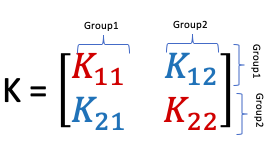
\includegraphics{kernel.png}
    \end{figure}
 where $K_{ij}$ is a collection of kernel matrix elements between samples from group $i$ and group $j$. Then $w(\sigma)$ corresponds to the mean of quantities in the diagonal clusters $K_{11}$ and $K_{22}$. $b(\sigma)$ is the mean of elements in the off-diagonal clusters (i.e. $K_{12}$ and $K_{21}$). Then we choose $\sigma$ that maximises $J(\sigma)$. 

For LFDA and KLFDA, one needs to select the dimensionality of the reduced space before implementation. We use a cross-validation procedure to choose from a range of dimensions. To save computational costs, a small subset of samples are split into, say, 5 folds. For each dimension, we train the LFDA/KLFDA with the 4 training folds then use its results to transform the features in the test fold. In the reduced space, a one-nearest-neighbour classifier is applied to the test samples, then the misclassification rate is computed. We repeat these steps on each of the CV test folds and select the dimension that minimises the average misclassification rate.

Theoretically, to choose the optimal number of types for each class of labels in SNMF (section \ref{Choose The Number of Types}), it is required to perform cross-validation on all possible dimensions. However, in this dataset the feature dimension is large and makes the algorithm computationally expensive. To ease the computational burden, we use the results of other dimension reduction methods to set an upper limit on the number of types that each class is allowed to keep in the reduced space. Hence, we perform CV up to a small number of dimensions, rather than all dimensions of the genotypes.

\subsection{Results}
With each set of estimated weights, we fit a LASSO logistic regression using the European samples. The LASSO tends to give sparse solutions, which is compatible to the prior knowledge that a phenotype is only associated to a small subset of genotypes. A logistic regression is preferred since the phenotypes are binary. Then we use the model to predict the phenotypes for the African samples. The results are shown in table \ref{simulated data res}. Furthermore, the weight estimates may have a large range, causing a large variance on predictive performance. Thus, one may consider using the exponentially-flattened importance weights, defined as $\hat{\beta}(x)^{\gamma}$, where $\gamma \in [0,1]$ is the exponential flattening parameter. $\gamma = 0$ reduces the model to a standard LASSO whereas $\gamma = 1$ refers to the unflattened weights. Choosing $0 < \gamma < 1 $ will give an intermediate estimator that balances the trade-off between statistical efficiency and consistency. Results with $\gamma = 0.5$ are given in table \ref{simulated data res flat}.

In this example, LFDA along with KLIEP yields similar results as the default setting where the weights all equal 1. This is because this model predicts the most sample wights to be close to 1 (see Figure \ref{sim_den}). Methods with KSPCA and SNMF assign zero weights to the majority of samples, which significantly reduce the size of effective training samples and lead to poor predictive performance. Some models (such as KSPCA + KLEIP and KSPCA + uLSIF) failed to provide predictions due to possibly numerical instability and small dimensionality of the dimension reduced space, further details will be discussed in the end of Chapter \ref{bio res}. The model KSPCA + KMM and model KLFDA + KLIEP are essentially intercept-only models. This is due to the number of samples the model trained upon is too small. In the exponentially-flattened case, the LASSO also reduces all regression coefficients in KLFDA + KLIEP to zero, although this model has fewer training samples with zero weights. Methods using LFDA tends to be more effective on this dataset, possibly due to a relatively large effective sample size. In this experiment, the exponentially-flattened weights indeed have a smaller variance comparing to the raw wights, however, this does not lead to an improved model performance. One explanation is that when the density-ratios are estimated poorly, all flattened weights are also unreliable and then covariate shift adaptation fails work.

 \begin{table}[H]
	\centering
\begin{tabular} {c | c | c | c | c }
method & AUC & sensitivity & specificity & accuracy  \\
\hline \hline
 default & 0.651 & 0.393 & 0.801 & 0.700 \\
 KLFDA + KLIEP& 0.5 & 1 & 0 & 0.245 \\
 KLFDA + KMM & 0.511 & 0.344 & 0.665 & 0.586 \\
 KLFDA + ULSIF& 0.531 & 0.635 & 0.419 & 0.472 \\
 KSPCA + KMM & 0.5 & 1 & 0 & 0.245 \\
 \textbf{LFDA + KLIEP} & 0.655 & 0.295 & 0.802 & 0.702 \\
 LFDA + KMM & 0.621 & 0.362 & 0.791 & 0.685  \\
 LFDA + ULSIF & 0.652 & 0.388 & 0.800 & 0.698 \\
 SNMF + KMM & 0.546 & 0.400 & 0.678 & 0.609 \\
 SPCA + KLIEP & 0.587  & 0.337 & 0.782 & 0.673 \\
 SPCA + KMM & 0.592  & 0.338 & 0.783 & 0.673 \\
 SPCA + ULSIF & 0.593 & 0.342 & 0.784 & 0.675 \\
\hline \hline
\end{tabular}	
\caption{Model performance on the simulated dataset using the raw density-ratio estimates. Default corresponds to weights all equal to 1.}
\label{simulated data res}
\end{table}

\begin{table}[H]
	\centering
\begin{tabular} {c | c | c | c | c }
method & AUC& sensitivity & specificity & accuracy  \\
\hline \hline
 \textbf{default} & 0.651 & 0.393 & 0.801 & 0.700 \\
 KLFDA + KLIEP& 0.5 & 1 & 0 & 0.245 \\
 KLFDA + KMM & 0.497 & 0.247 & 0.752 & 0.628 \\
 KLFDA + ULSIF& 0.592 & 0.316 & 0.776 & 0.662  \\
 KSPCA + KMM & 0.502 & 0.268 & 0.731 & 0.617 \\
 \textbf{LFDA + KLIEP} & 0.651 & 0.392 & 0.801 & 0.700  \\
 LFDA + KMM & 0.640 & 0.382 & 0.797 & 0.695 \\
 LFDA + ULSIF & 0.651 & 0.390 & 0.800 & 0.699 \\
 SNMF + KMM & 0.540 & 0.276 & 0.763 & 0.643 \\
 SPCA + KLIEP & 0.611 & 0.346 & 0.786 & 0.677 \\
 SPCA + KMM & 0.615 & 0.350 & 0.787 & 0.679 \\
 SPCA + ULSIF & 0.615 & 0.362 & 0.791 & 0.685 \\
\hline \hline
\end{tabular}	
\caption{Model performance on the simulated dataset using the flattened weights ($\gamma = 0.5$).}
\label{simulated data res flat}
\end{table}

\begin{figure}[H]
\begin{subfigure}{.32\textwidth}
  \centering
  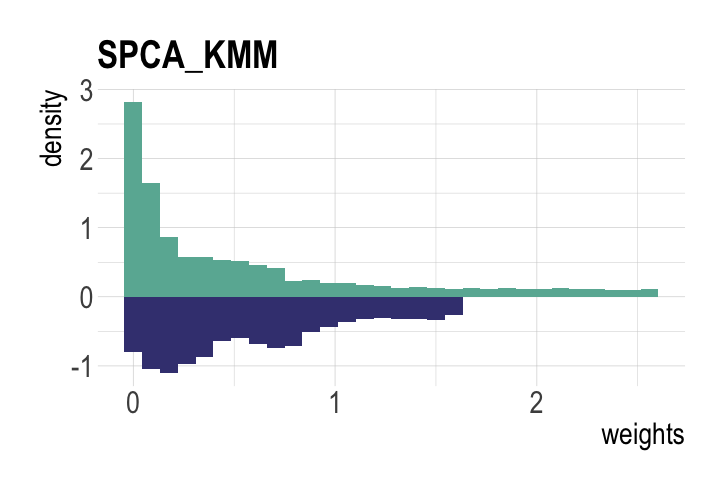
\includegraphics[width=\linewidth]{toy1.png}
  \label{fig:sfig1}
\end{subfigure}
\begin{subfigure}{.32\textwidth}
  \centering
  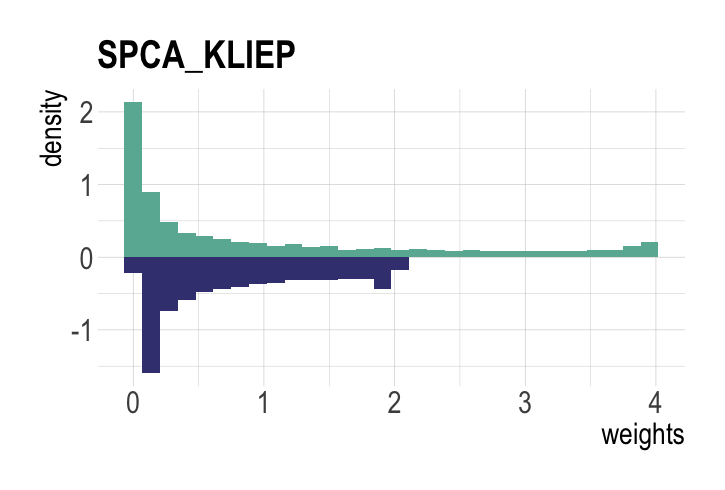
\includegraphics[width=\linewidth]{toy2.png}
  \label{fig:sfig2}
\end{subfigure} 
\begin{subfigure}{.32\textwidth}
  \centering
  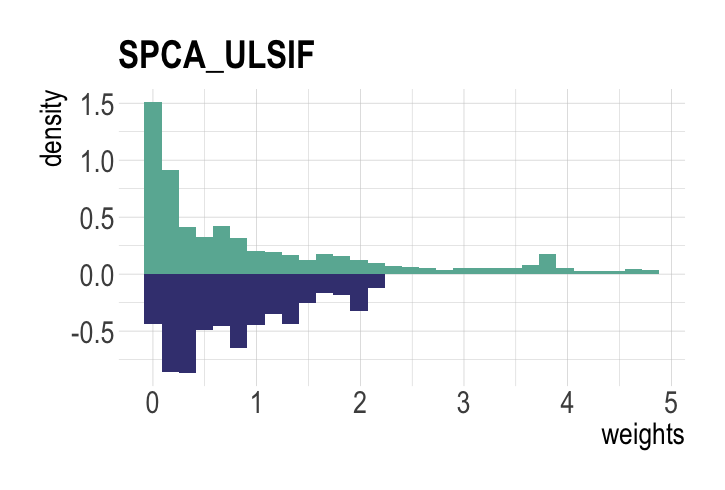
\includegraphics[width=\linewidth]{toy3.png}
  \label{fig:sfig1}
\end{subfigure}
\begin{subfigure}{.32\textwidth}
  \centering
  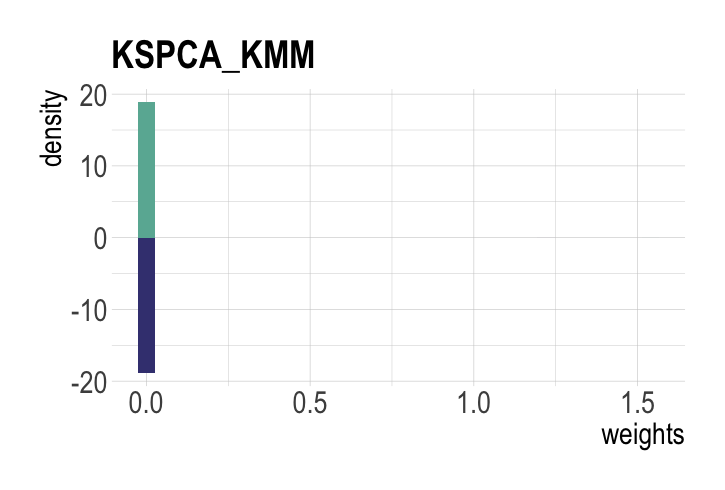
\includegraphics[width=\linewidth]{toy4.png}
  \label{fig:sfig2}
\end{subfigure} %
\begin{subfigure}{.32\textwidth}
  \centering
  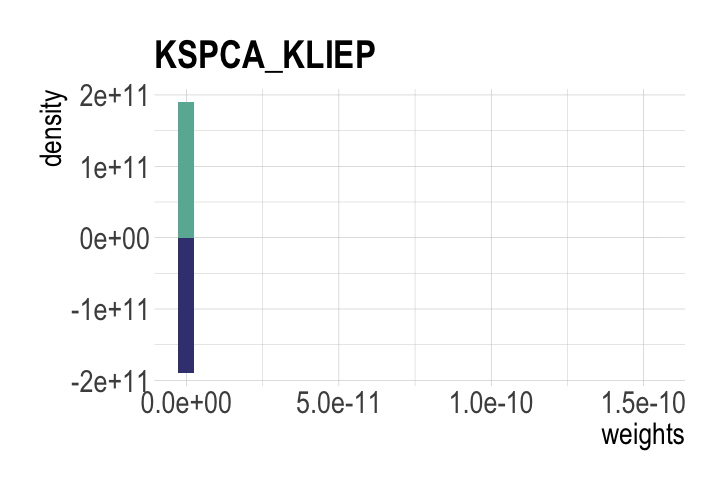
\includegraphics[width=\linewidth]{toy5.png}
  \label{fig:sfig1}
\end{subfigure}%
\begin{subfigure}{.32\textwidth}
  \centering
  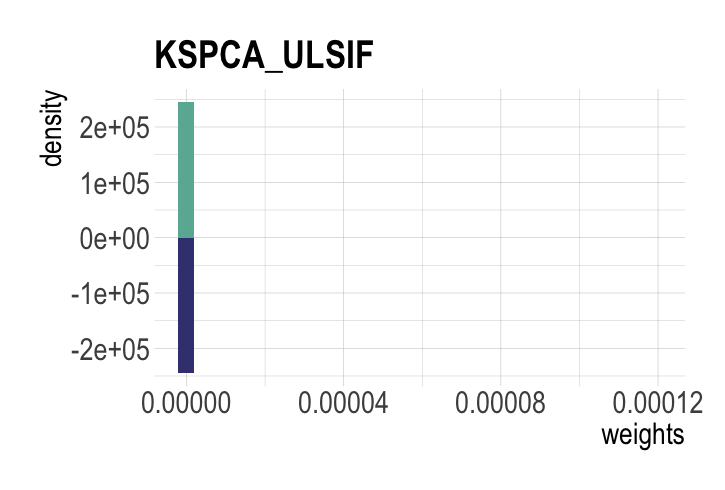
\includegraphics[width=\linewidth]{toy6.png}
  \label{fig:sfig2}
\end{subfigure} 
\begin{subfigure}{.32\textwidth}
  \centering
  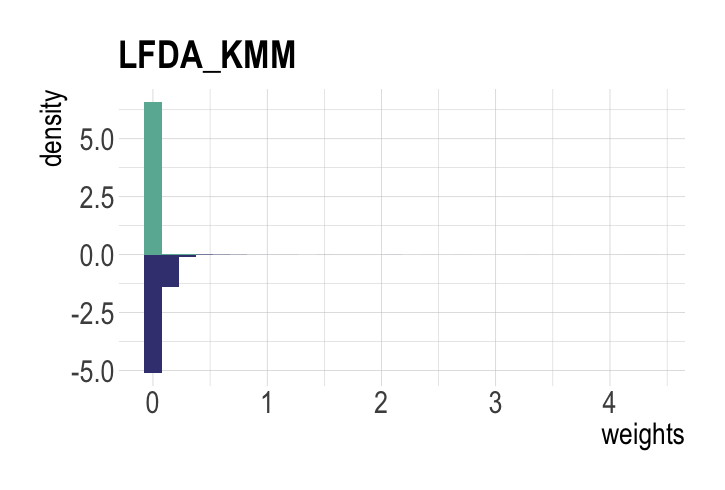
\includegraphics[width=\linewidth]{toy7.png}
  \label{fig:sfig1}
\end{subfigure}
\begin{subfigure}{.32\textwidth}
  \centering
  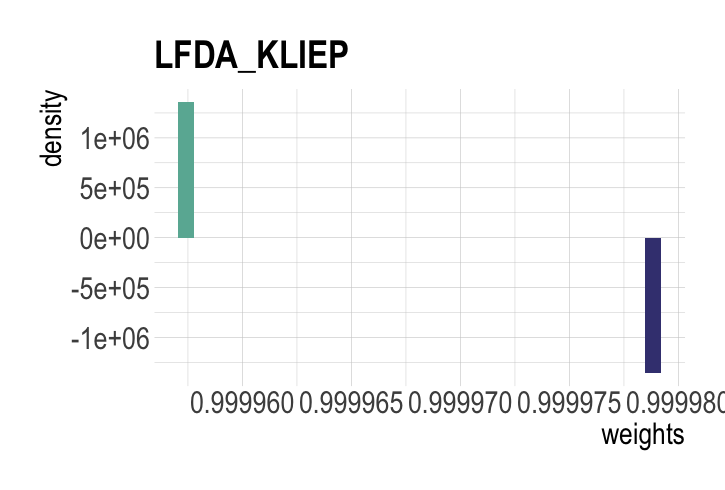
\includegraphics[width=\linewidth]{toy8.png}
  \label{fig:sfig2}
\end{subfigure} 
\begin{subfigure}{.32\textwidth}
  \centering
  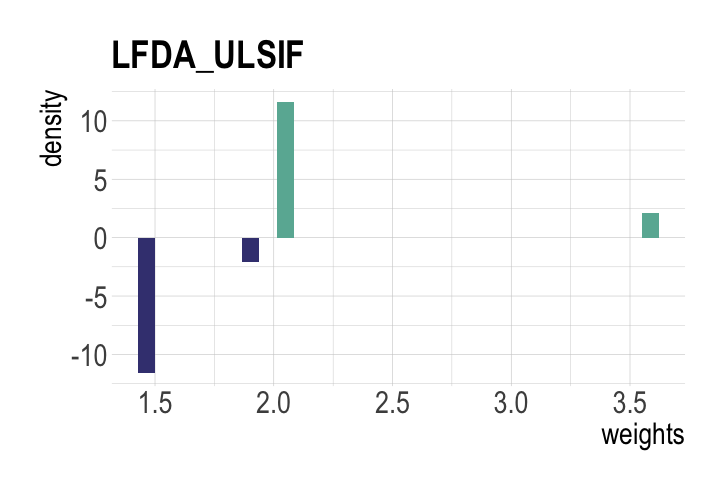
\includegraphics[width=\linewidth]{toy9.png}
  \label{fig:sfig1}
\end{subfigure}
\begin{subfigure}{.32\textwidth}
  \centering
  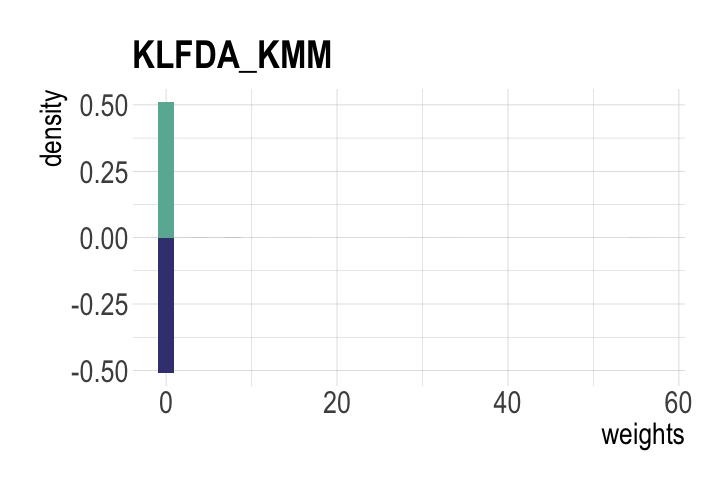
\includegraphics[width=\linewidth]{toy10.png}
  \label{fig:sfig2}
\end{subfigure} %
\begin{subfigure}{.32\textwidth}
  \centering
  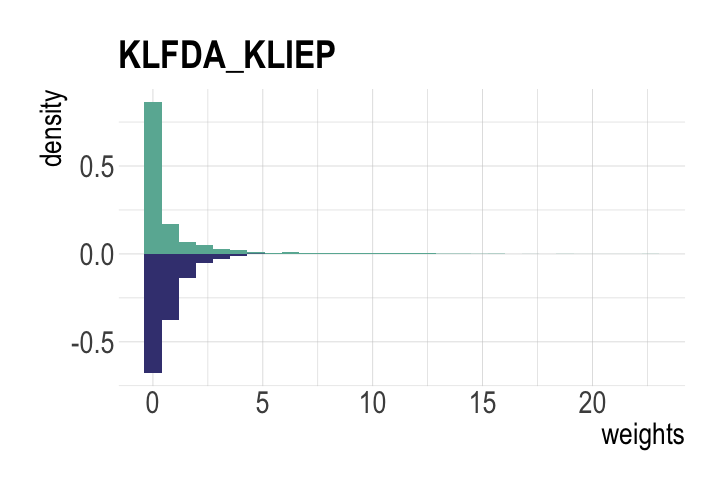
\includegraphics[width=\linewidth]{toy11.png}
  \label{fig:sfig1}
\end{subfigure}%
\begin{subfigure}{.32\textwidth}
  \centering
  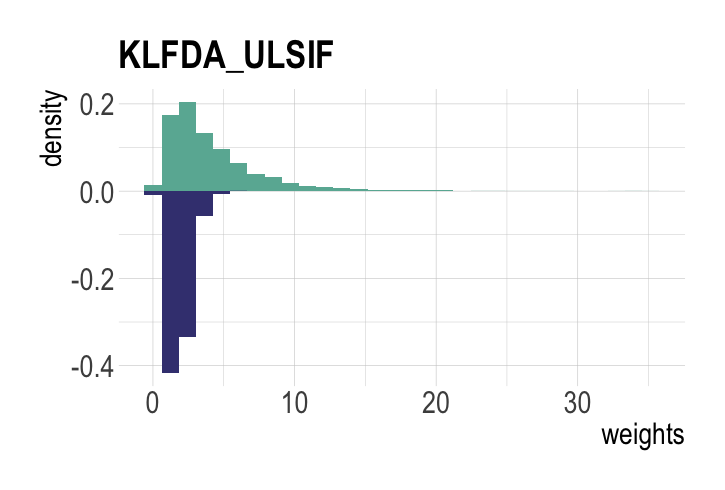
\includegraphics[width=\linewidth]{toy12.png}
  \label{fig:sfig2}
\end{subfigure} 
\begin{subfigure}{.32\textwidth}
  \centering
  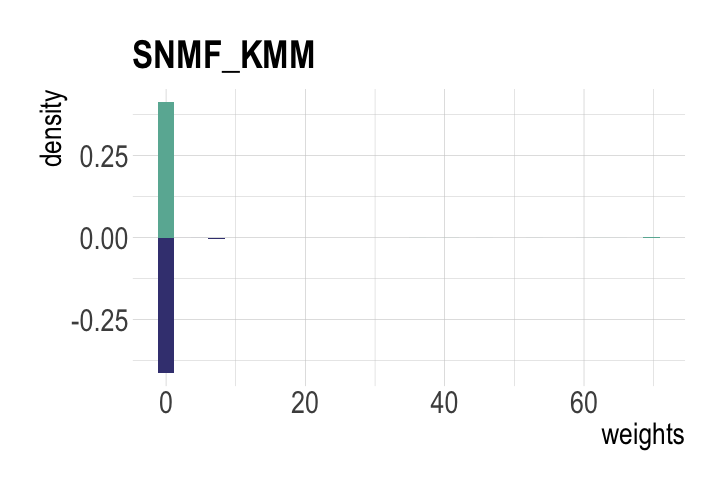
\includegraphics[width=\linewidth]{toy13.png}
  \label{fig:sfig2}
\end{subfigure} %
\begin{subfigure}{.32\textwidth}
  \centering
  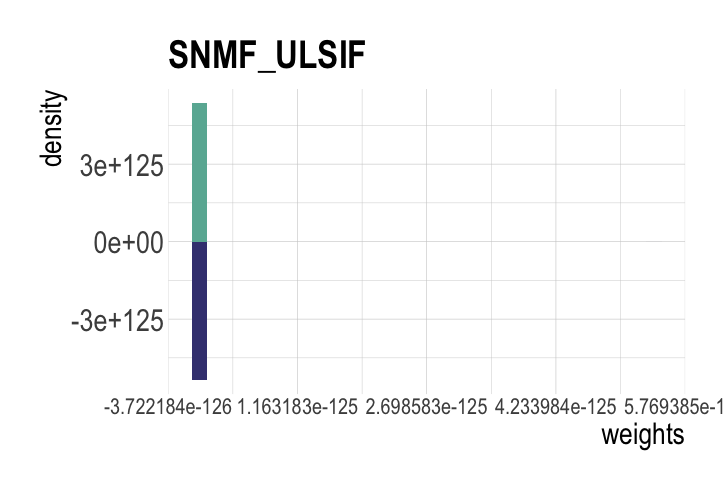
\includegraphics[width=\linewidth]{toy14.png}
  \label{fig:sfig1}
\end{subfigure}%
\begin{subfigure}{.32\textwidth}
  \centering
  
\includegraphics[width=.6\linewidth]{toy15.png}
  \label{fig:sfig2}
\end{subfigure} %
\caption{Each mirrored histogram represents a set of weight estimates. The upper half in green indicates the raw weights, the lower half in blue indicates the exponentially-flattened weights with $\gamma = 0.5$.}
\label{sim_den}
\end{figure} 

\pagebreak
%
%
%
%=============================================================
% data
%=============================================================
%
%
%
\section{Experiment on the UK Biobank Dataset} \label{Data}
\subsection{Data} \label{biodata}
The Quality Controlled UK Biobank genomic data consists of genome-wide genotype data from 406,263 individuals across the United Kingdom [\cite{bycroft2018uk}]. Among all participants, 219,135 are female (54\%) and 187,128 are male (46\%). At the time they registered the project, the youngest participant aged 49 and the eldest aged 83, half of the samples have age between 61 and 75. The blood, urine and saliva samples from each participant were provided, physical measurements were recorded (such as height, BMI, waist circumference etc.) along with a questionnaire focusing on their health and lifestyle (including whether each individual is diagnosed to asthma, breast cancer, prostate cancer, type II diabetes, high cholesterol, high blood pressure etc.). The genotypes of individuals were assayed using two Affymetrix platforms: 364,666 samples (89.8\%) in the Applied Biosystems UK Biobank Axiom Array and the rest 41,597 samples (10.2\%) in the UK BiLEVE Axiom. A series of Quality Control measures have been carried out, for instance (1) the overall missing rate of each remaining genotype cannot exceed 5\% (2) minor allele frequencies (MAF) is at least 0.0001 (3) the missing call rate for each individual cannot exceed 10\% [\cite{biobank2015genotyping}], which leaves us 784,256 genotypes that meet the criterion. Here are 4 important features related to this dataset that may affect our design of methods and experiment, which are illustrated as the following:

First, the size of this dataset is unprecedented in biomedical science field, and hence it provides the opportunity for a better understanding of human biology and diseases. However, it has also raised analytical challenges: although genotypes only take value from 0,1 and 2 and a large proportion are 0, meaning that this giant genotype array can be stored as a sparse matrix and hence ease the memory needed for storing it, the size of this matrix is still too significant and takes more than 1200 Gb of storage. Additionally, computation required for analysis grows with the number of samples and the size of variables (and depending on the complexity of algorithms, it can sometimes grow exponentially). Given the size of the matrix, this limits the range of algorithms can be implemented. Hence, one needs to carefully design the sampling method such that the validity of analysis is not weakened, and ensure that any algorithms employed are computationally feasible. 

Second, this dataset is highly imbalanced in the ethnic background of participants: 94\% participants reported their ethnicity as group "White" and remarkably, 93\% of them are British. A list containing the detailed information about the samples' ethnicity is shown in table \ref{ethnicity}. This disproportionality in populations means that estimating using this data may be appropriate for White populations but cannot be transferred to other ethnic groups.

\begin{table}[h]
	\centering
\begin{tabular} {c | c | c | c }
\multicolumn{2}{c}{self-reported ethnicity} & \multicolumn{2}{c}{proportion(\%)}  \\
\hline \hline
White & & 93.81 &   \\
 & British &  & 87.45  \\
 & Irish &  & 2.62  \\
 & Any other White background &  & 3.74  \\
 \hline
 Asian & & 2.11 & \\
 & Indian & & 1.26 \\
 & Pakistani & & 0.39 \\
 & Bangladeshi & & 0.05 \\
 & Any other Asian background & & 0.41 \\
 \hline
  Chinese & & 0.35 \\
  \hline
 Black & & 1.72 & \\
 & African & & 0.76 \\
 & Caribbean & & 0.93 \\
 & Any other Black background & & 0.03 \\
 \hline
 Mixed & & 0.63 & \\
 & White and Asian & & 0.18 \\
 & White and Black African  & & 0.09 \\
 & White and Black Caribbean & & 0.13 \\
 & Any other mixed background & & 0.23 \\
 \hline
Other/Unknown & & 1.38 &\\
\hline \hline
\end{tabular}	
\caption{Self-reported ethnicity categories in the 406,263 UK Biobank samples.}
\label{ethnicity}
\end{table}

Third, the genotypes vary noticeably among different ethnic backgrounds. Principal component analysis (PCA) applied to the genotype matrix can be used to capture the population structure. The 10 major PCs are plotted in consecutive pairs (see figure \ref{fig:fig}) illustrating that populations from the similar ancestries also have the similar principal component scores. In particular,  the PC1 and PC2 separates out the Black and Black British samples, whereas PC3 and PC4 indicates Asian and Asian British. These results demonstrate the importance of accounting for ethnic background in related genetic analysis. Otherwise the minority groups may be treated as random noise or outliers, reducing the model's performance.

\begin{figure}[h]
\begin{subfigure}{.32\textwidth}
  \centering
  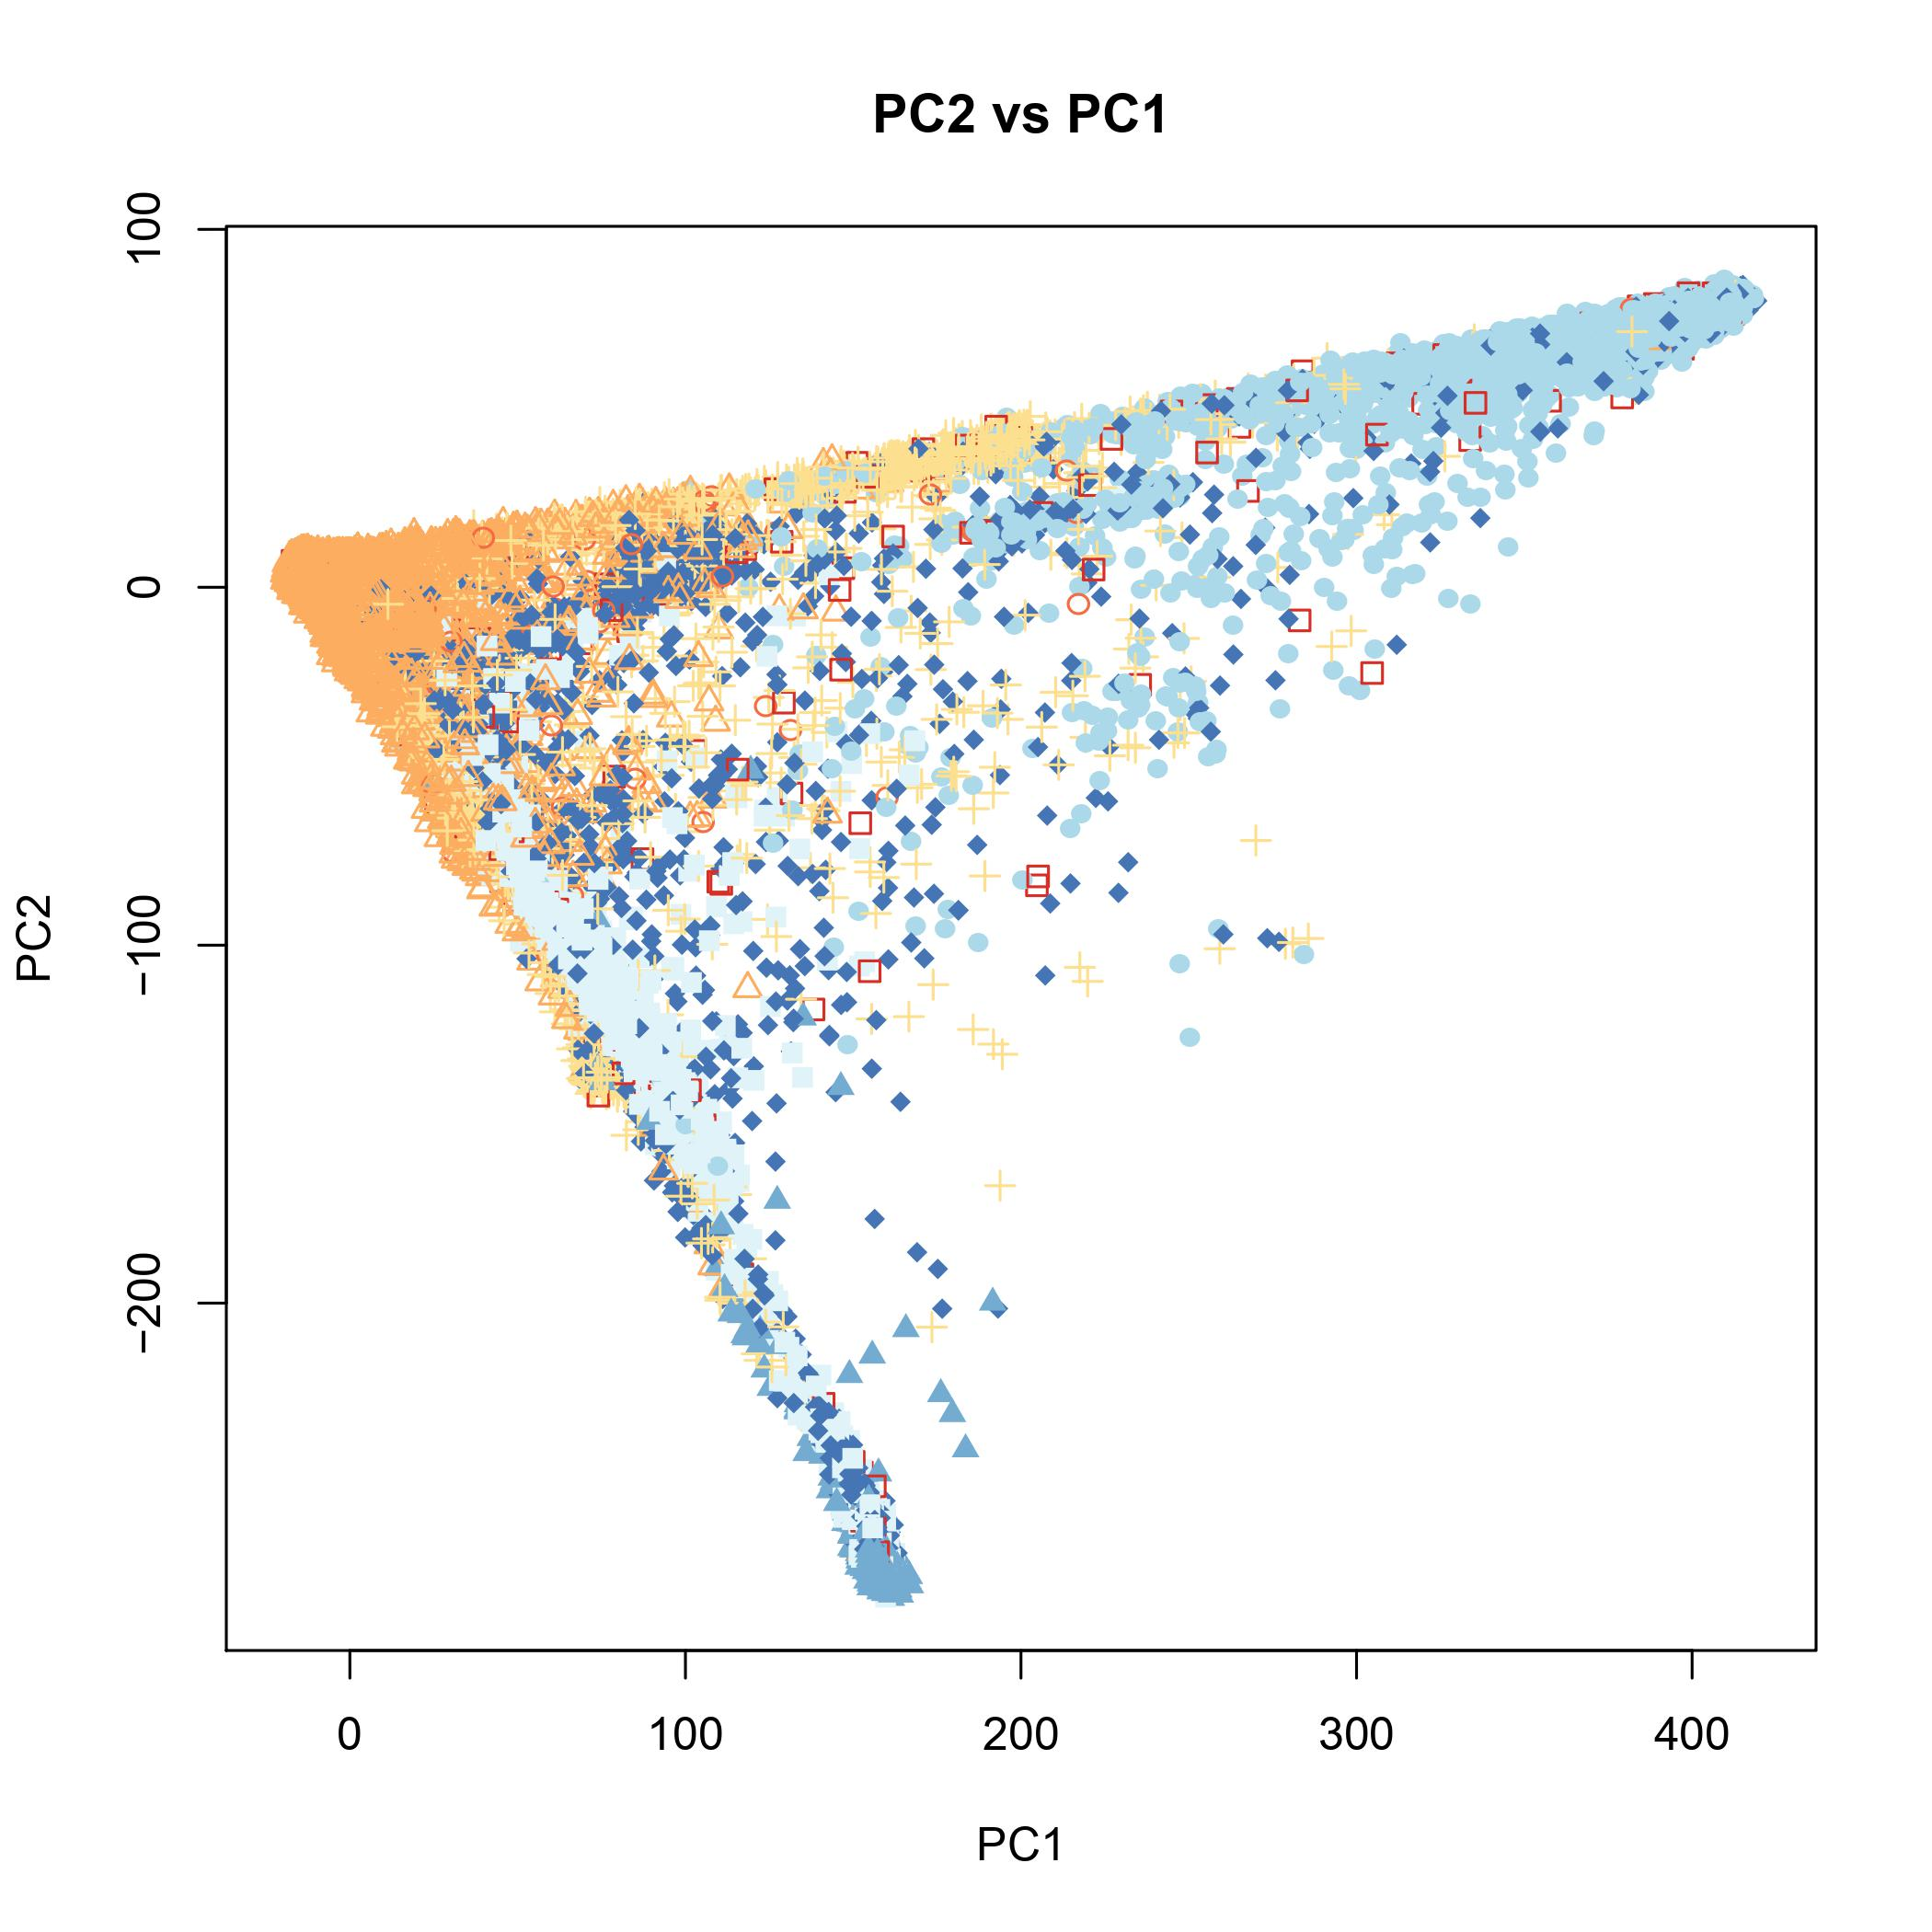
\includegraphics[width=\linewidth]{pca1_2.jpg}
  \label{fig:sfig1}
\end{subfigure}
\begin{subfigure}{.32\textwidth}
  \centering
  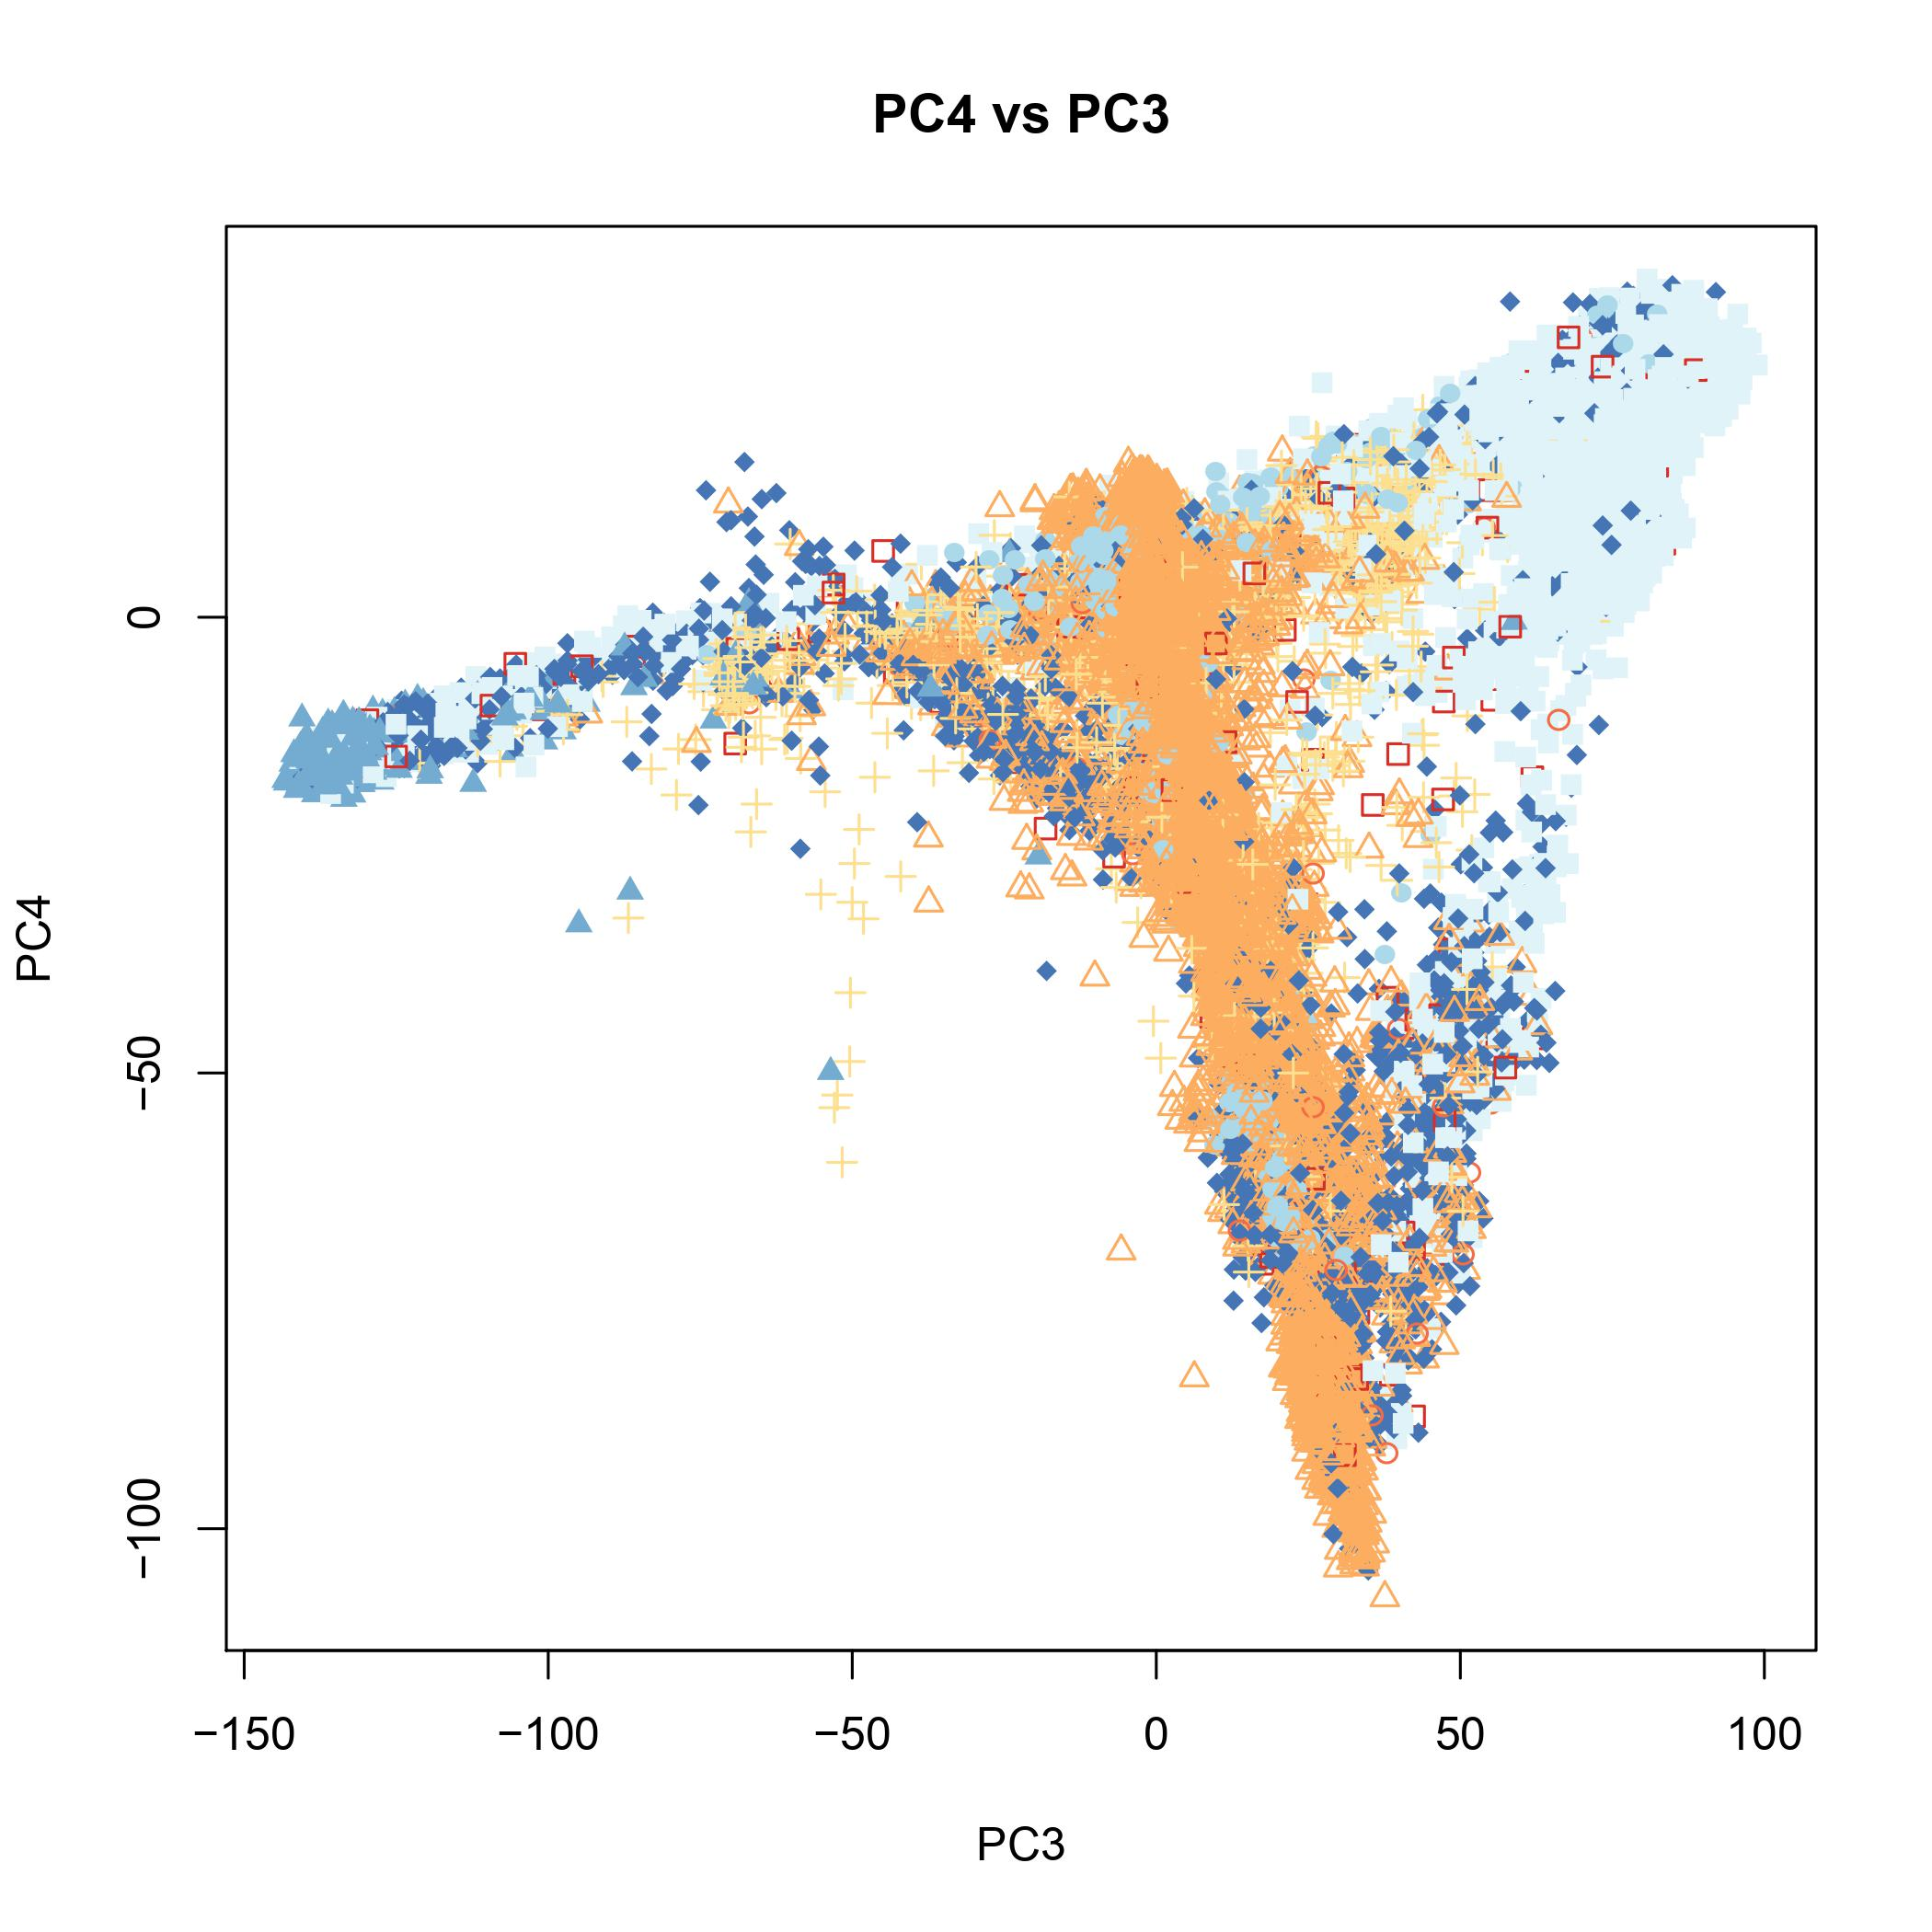
\includegraphics[width=\linewidth]{pca3_4.jpg}
  \label{fig:sfig2}
\end{subfigure} 
\begin{subfigure}{.32\textwidth}
  \centering
  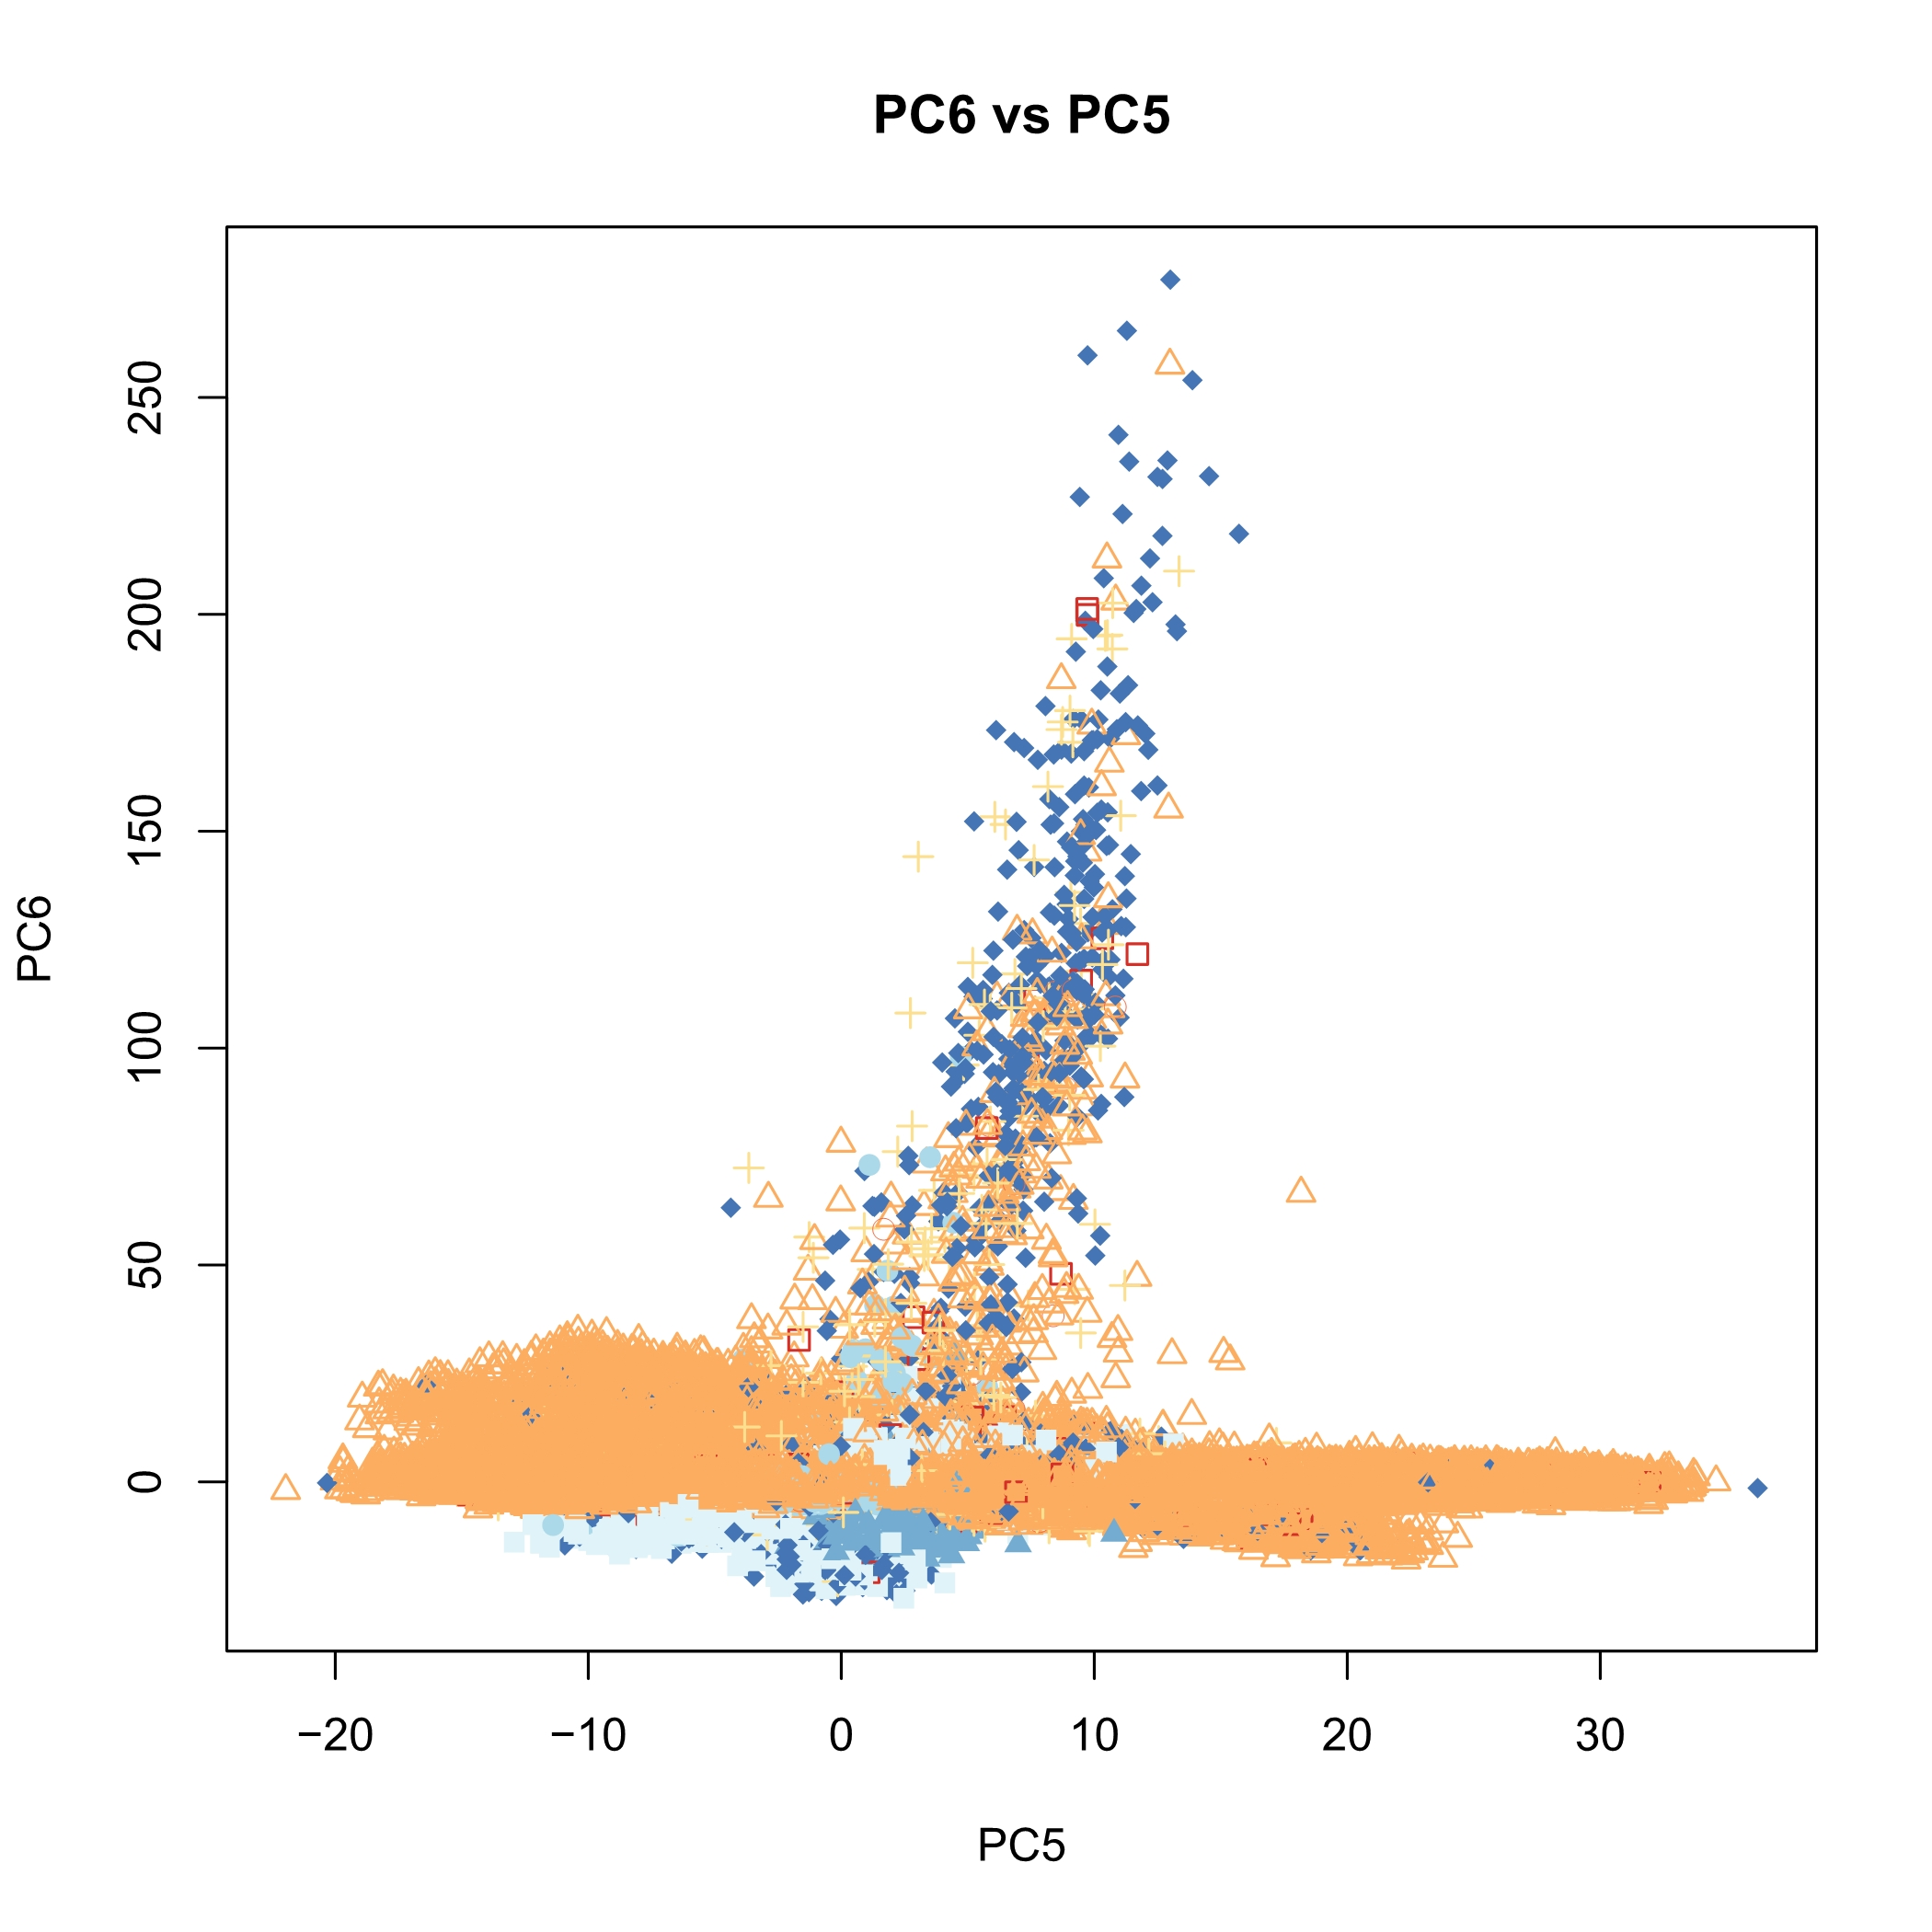
\includegraphics[width=\linewidth]{pca5_6.jpeg}
  \label{fig:sfig1}
\end{subfigure}
\begin{subfigure}{.32\textwidth}
  \centering
  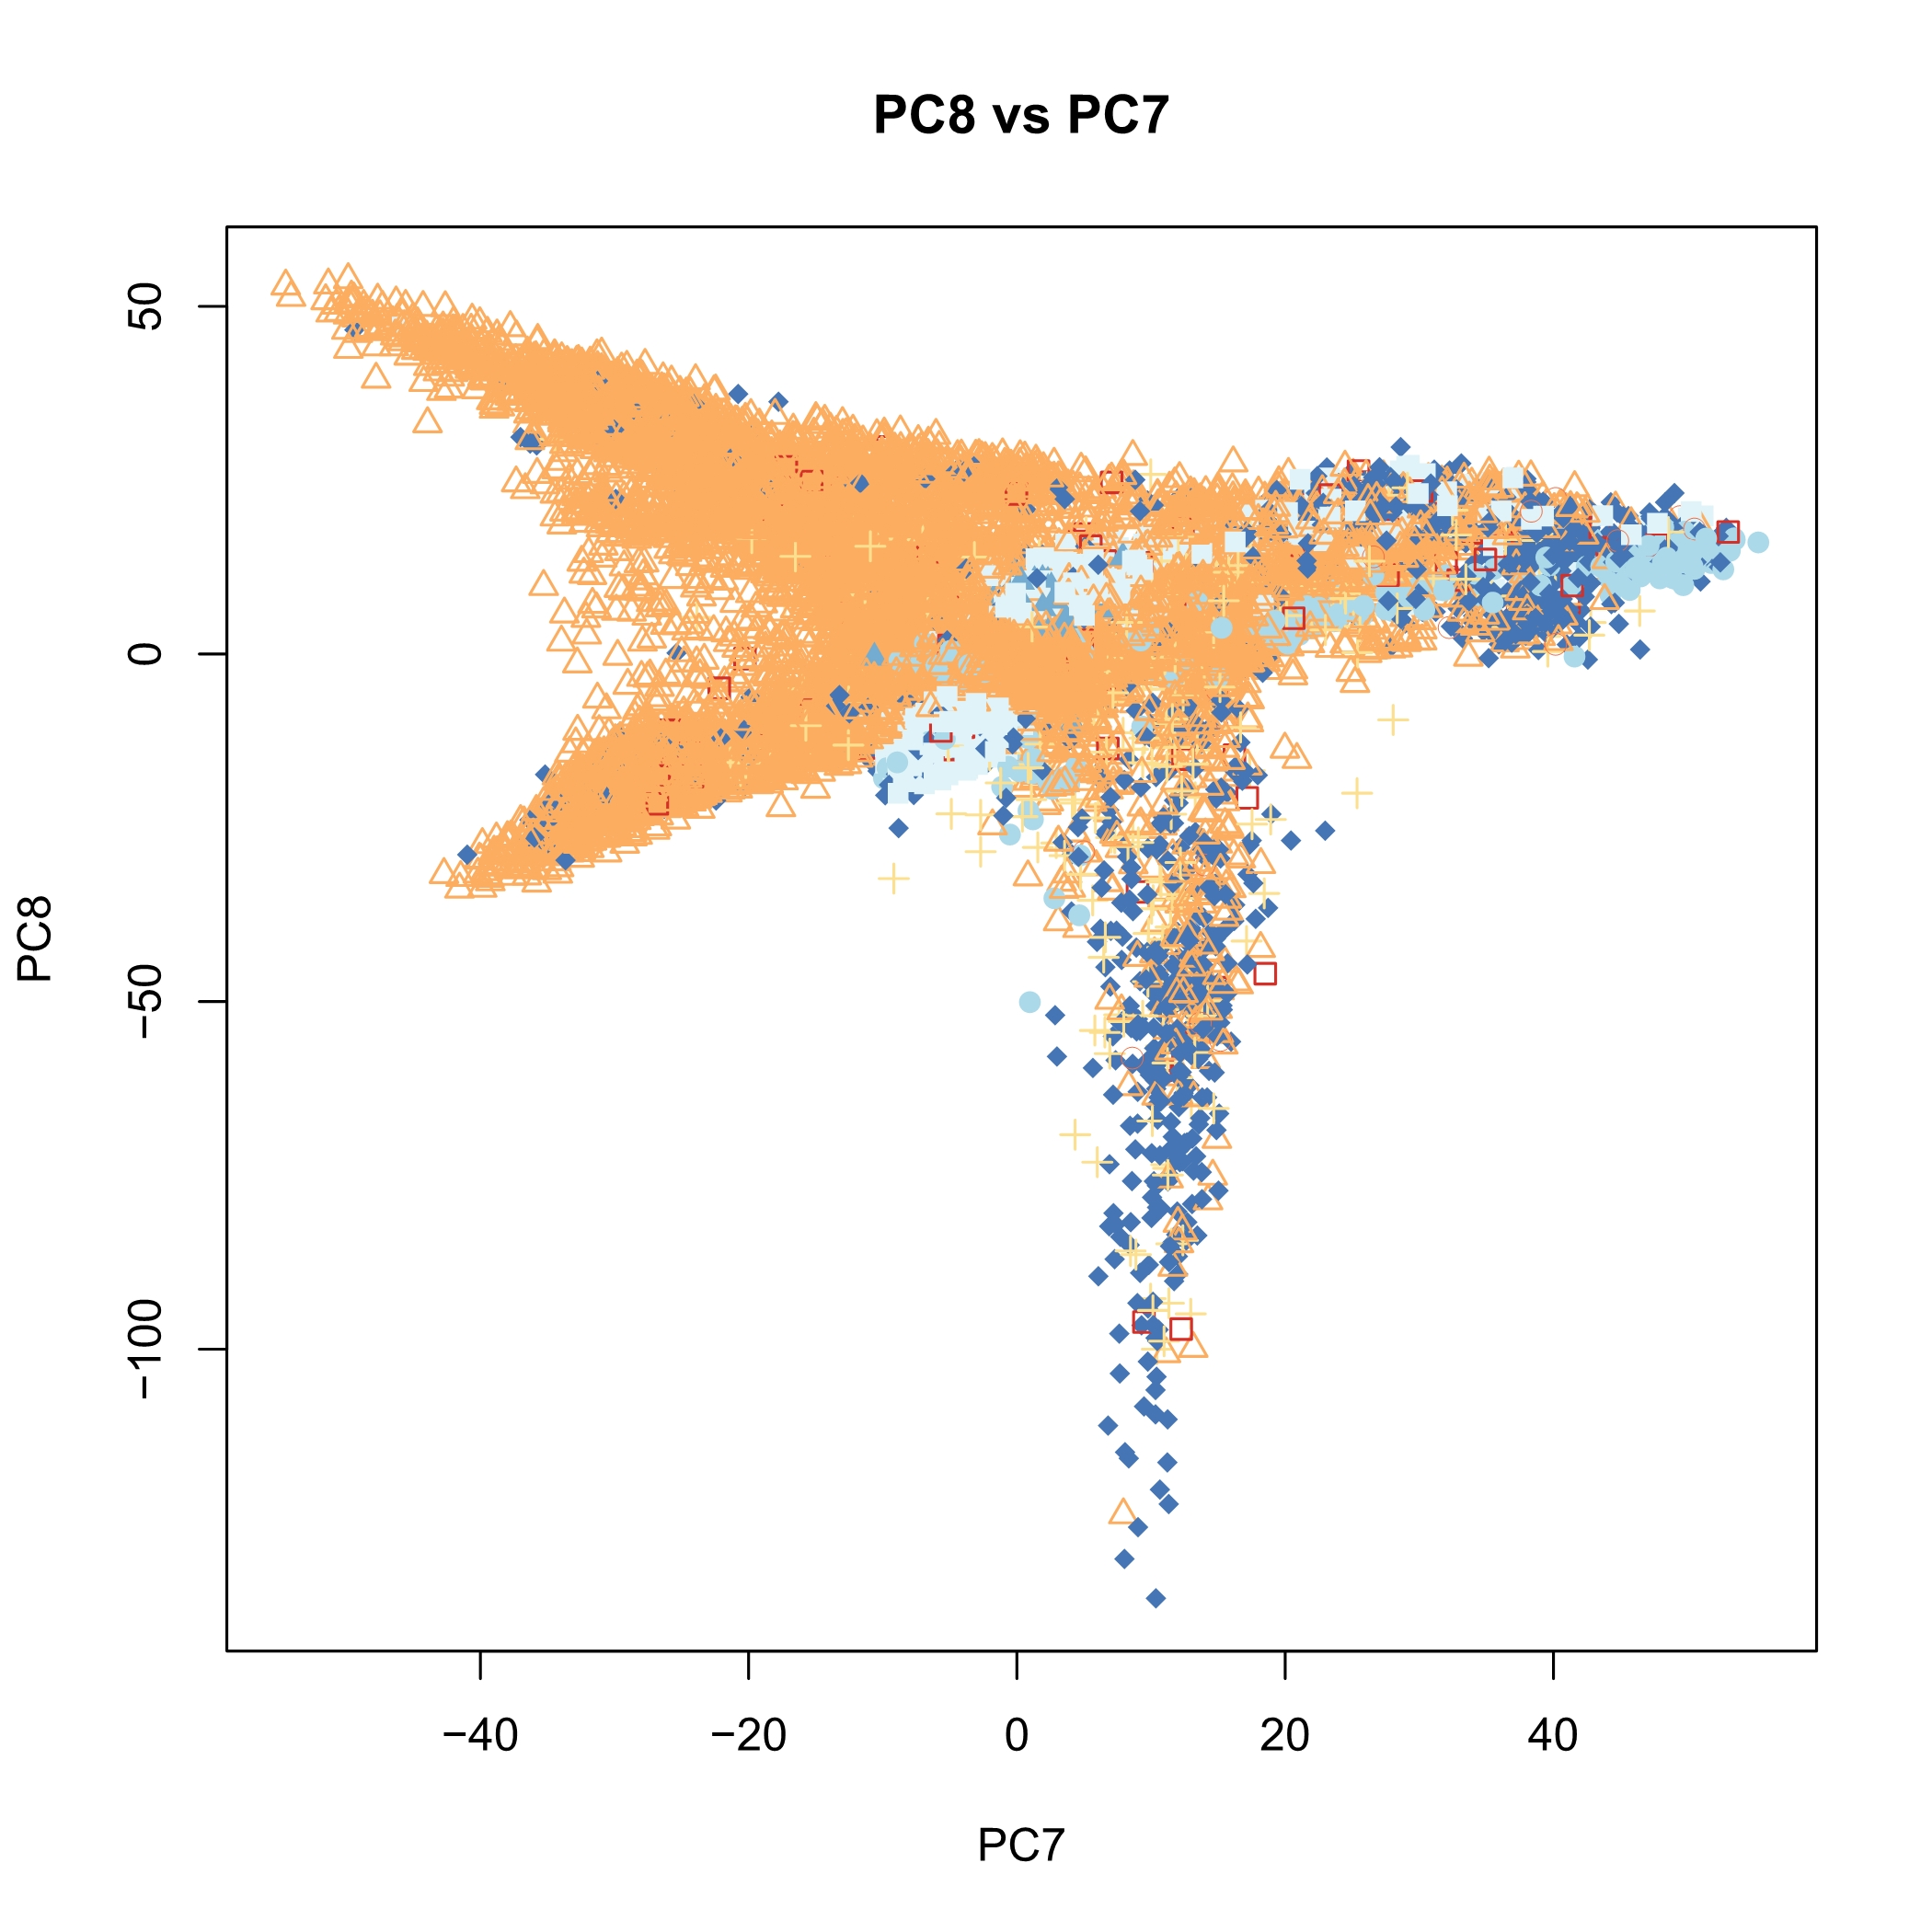
\includegraphics[width=\linewidth]{pca7_8.jpeg}
  \label{fig:sfig2}
\end{subfigure} %
\begin{subfigure}{.32\textwidth}
  \centering
  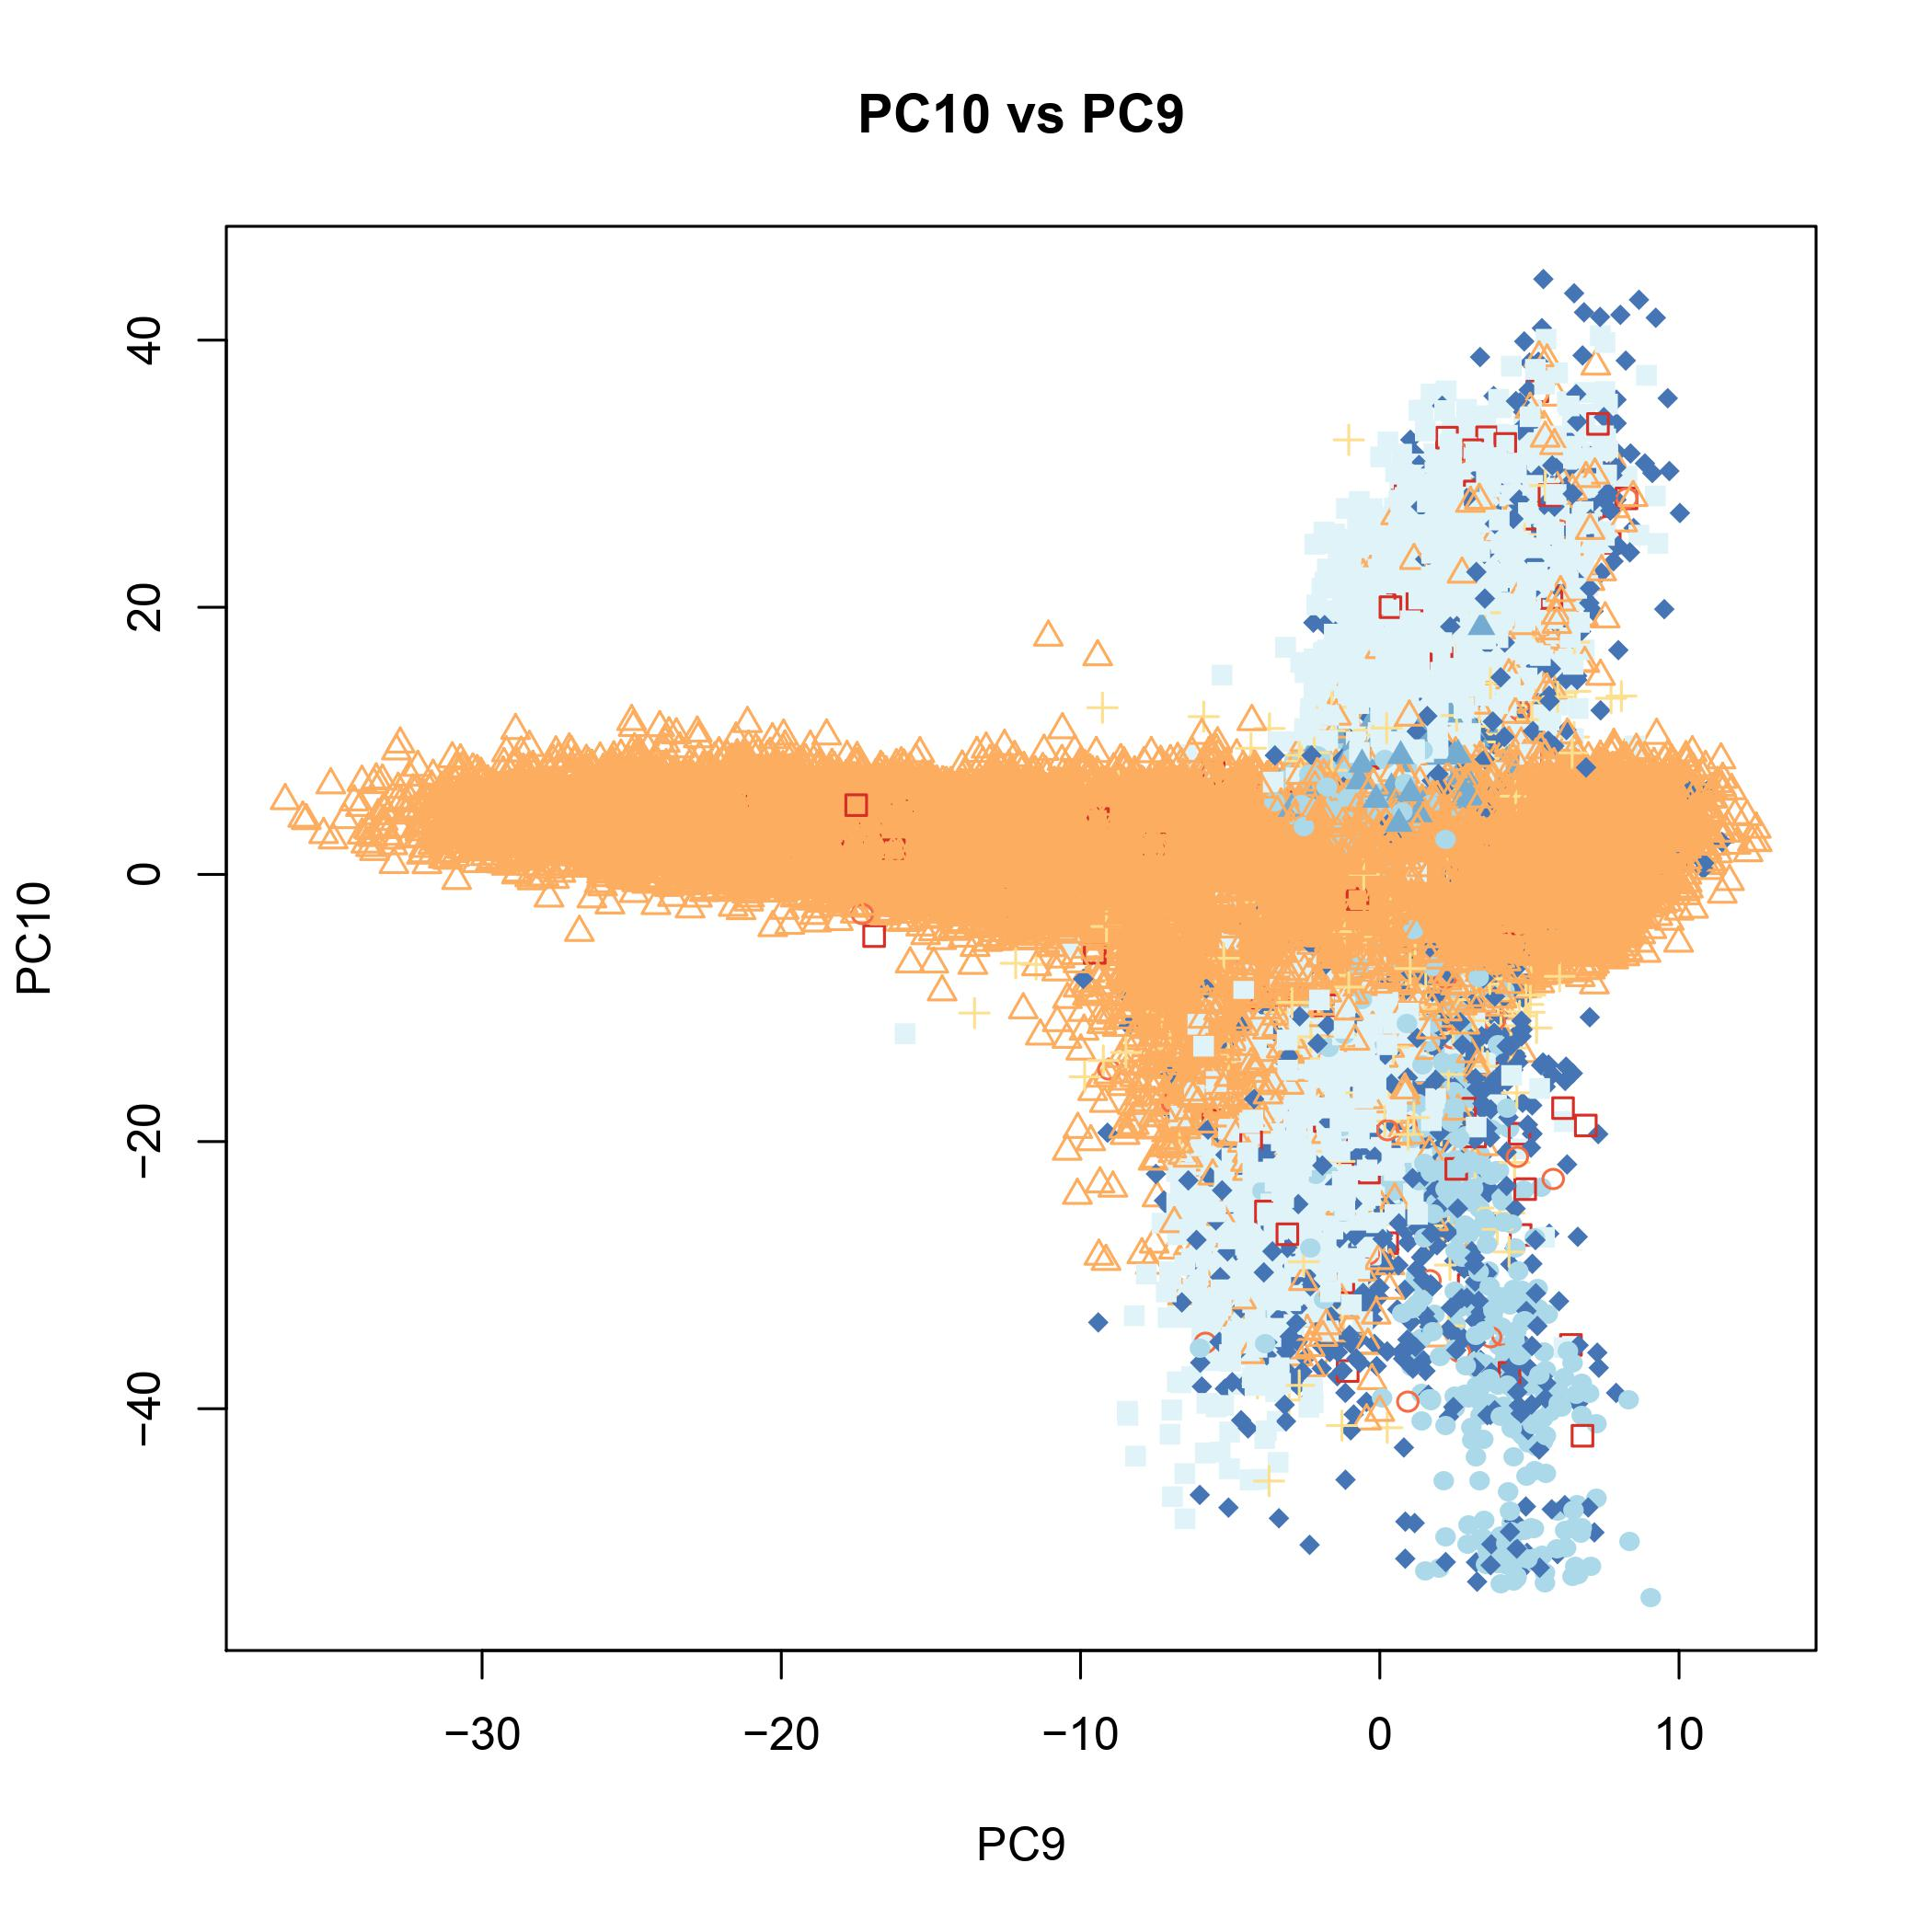
\includegraphics[width=\linewidth]{pca9_10.jpg}
  \label{fig:sfig1}
\end{subfigure}%
\begin{subfigure}{.32\textwidth}
  \centering
  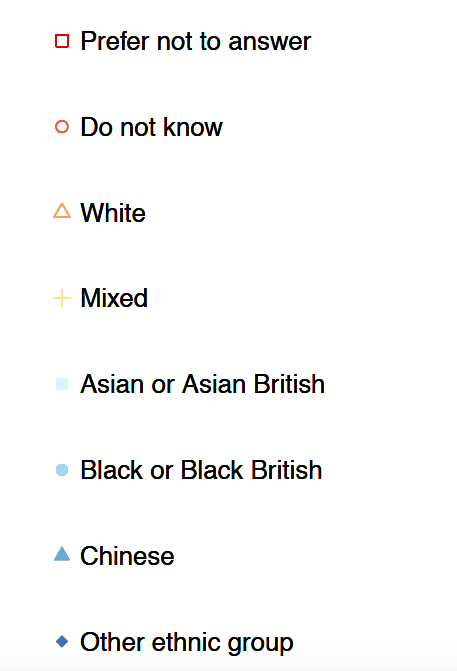
\includegraphics[width=.6\linewidth]{legend.png}
  \label{fig:sfig2}
\end{subfigure} %
\caption{First 10 PCs of all genotypes in the UK Biobank dataset, colours and shapes of points indicate the corresponding ethnic group.}
\label{fig:fig}
\end{figure} 

Typically, only a small fraction of genetic variants have a causal relationship to a specific phenotype. Using White British participants from UK Biobank, [\cite{canela2018atlas}] analysed the genetic associations for 118 non-binary and 599 binary traits by fitting linear mixture models. It shows that about one in 7,500 genotypes reached the conventional genome-wide significant thresholds ($P<10^{-8}$) for binary traits and one in about 300 genotypes was significant for non-binary traits. Thus, one may consider models that encourage sparse solutions or other screening methods that filters out non-significant variants.

\subsection{Experiment Design} \label{Experiment Design}
Ordinary machine learning algorithms split a dataset into training, validation and test samples, where the training data are used to learn the parameter, the validation samples are for comparing the performance of various models, then the test set is for computing an unbiased risk associated to the best performing model. However, in our dataset, considering the number of Black individuals is significantly smaller than the White individuals, the predictive risks may have a relatively large variance. To alleviate this, we use cross-validation, splitting the Black samples into 5 portions. Then we treat one portion as the test set and take the Black samples in the other four portions as training samples. To reflect the imbalance of the ethnicity in the whole dataset, we further scan the White samples and select ones that best match the current training set Black samples in gender and age, such that in the overall training set, Black samples count for a small proportion of total all participants, say, 20\%. Finally we repeat this procedure for each of the Black portions to obtain 5 train-test sets, for each test set only Black samples are included and each training set is a mix of Black and White samples where the latter holds the majority. Based on this train-test split, we can generate 5 separate predictive risk estimates, taking their mean for a more accurate assessment on effectiveness of the models. 

Each individual has 784,256 genotypes recorded. Combined with the large sample size, this makes the computation highly costly. Additionally, only a small number of variants are in fact causal to a phenotype. Hence we implement a pre-screening process to provide us a preliminary understanding about the importance of each variant. For a genotype $g$, we fit a linear regression denoted as $$Y=\beta_{x} \mathbf{X}+\beta_{g} g+\epsilon,$$ where $Y$ is the phenotype, $\epsilon$ is the noise that follows $N(0, \operatorname{var}[Y \mathbf{X}+g])$ and assuming this variance is constant across all samples. $X$ is a covariate matrix that contains variables: age and the first 10 PCs of all genotypes. Note that the PCs in the regression can be considered as an indicator of the population structure. We loop this over all genotypes and for each regression, collect the p-value of each genotype (which correspond to the null hypothesis that $\beta_{g}=0$) and rank these p-values, then only select ones which have small p-values. Theoretically, a logistic regression would be more appropriate since the disease phenotypes are binary. However, in practice, estimating coefficients through iteratively re-weighted least squares (IWLS) is computationally expensive especially given that we need to fit 780k+ regressions, hence linear regressions that are more simple to solve are used instead. We can reduce the computations by swapping the position of phenotype and genotype [\cite{voorman2012fast}], i.e. we fit the following model instead $$g=\gamma_{x} \mathbf{X}+\gamma_{y} Y+\xi.$$ This is valid because $\gamma_{y}=0$ is equivalent to $\beta_{g}=0$ in previous model and yields the same p-value. Whereas in the swapped model, the covariates for all regressions are unchanged so that the hat matrix, also other quantities that are solely dependent of the feature matrix only need to be computed once. To prevent data leakage, this pre-screening is applied to each train-test split separately. Then observations used to fit the regression are restricted to ones in each training set, then the results are deployed directly to the test set. In this experiment, we select 5\% of lowest p-value variants, which is about 40,000 in size.

The original dataset contains missing values due to a number of reasons.  For example, some variants are particularly complicated such that they are currently not supported by the genotyping analysis pipeline. Therefore, for each train-test split, genotypes that all values are missing in either training or test folds are removed. Also since we only keep a relatively small number of variants after screening, there would be cases, although rare, that two samples have exactly the same post-screening features. It is necessary to removed the duplicated samples, otherwise in later procedure, the kernel matrices constructed with the duplicated observations would be singular. For the rest of missing quantities, they are imputed with the mean value of its corresponding genotype.

Then for each train-test split, we apply the supervised dimension reduction methods on the training samples and employ the results onto the test samples. On the lower dimensional feature space, we then apply the density ratio estimation algorithms. We use the same algorithms to choose the Gaussian kernel width and the dimension of LFDA reduced space as in the artificial dataset (Chapter \ref{Implementation}). Once the weights for training samples are obtained, we fit the training samples into a LASSO logistic regression. To tune the LASSO regularisation parameter, we further split each training set into 5 inner folds and use cross-validation to tune the LASSO regularisation parameter, the average AUC across inner folds is used as our evaluation metric and the regularisation parameter with largest AUC is chosen. Once we have both the optimal regularisation parameter and training sample weights, we finally apply the LASSO logistic regression to make predictions on the test set, then evaluate the performance across different test folds. This experiment design is illustrated in Figure \ref{experiment png}.

\begin{figure}[H]
    \centering
    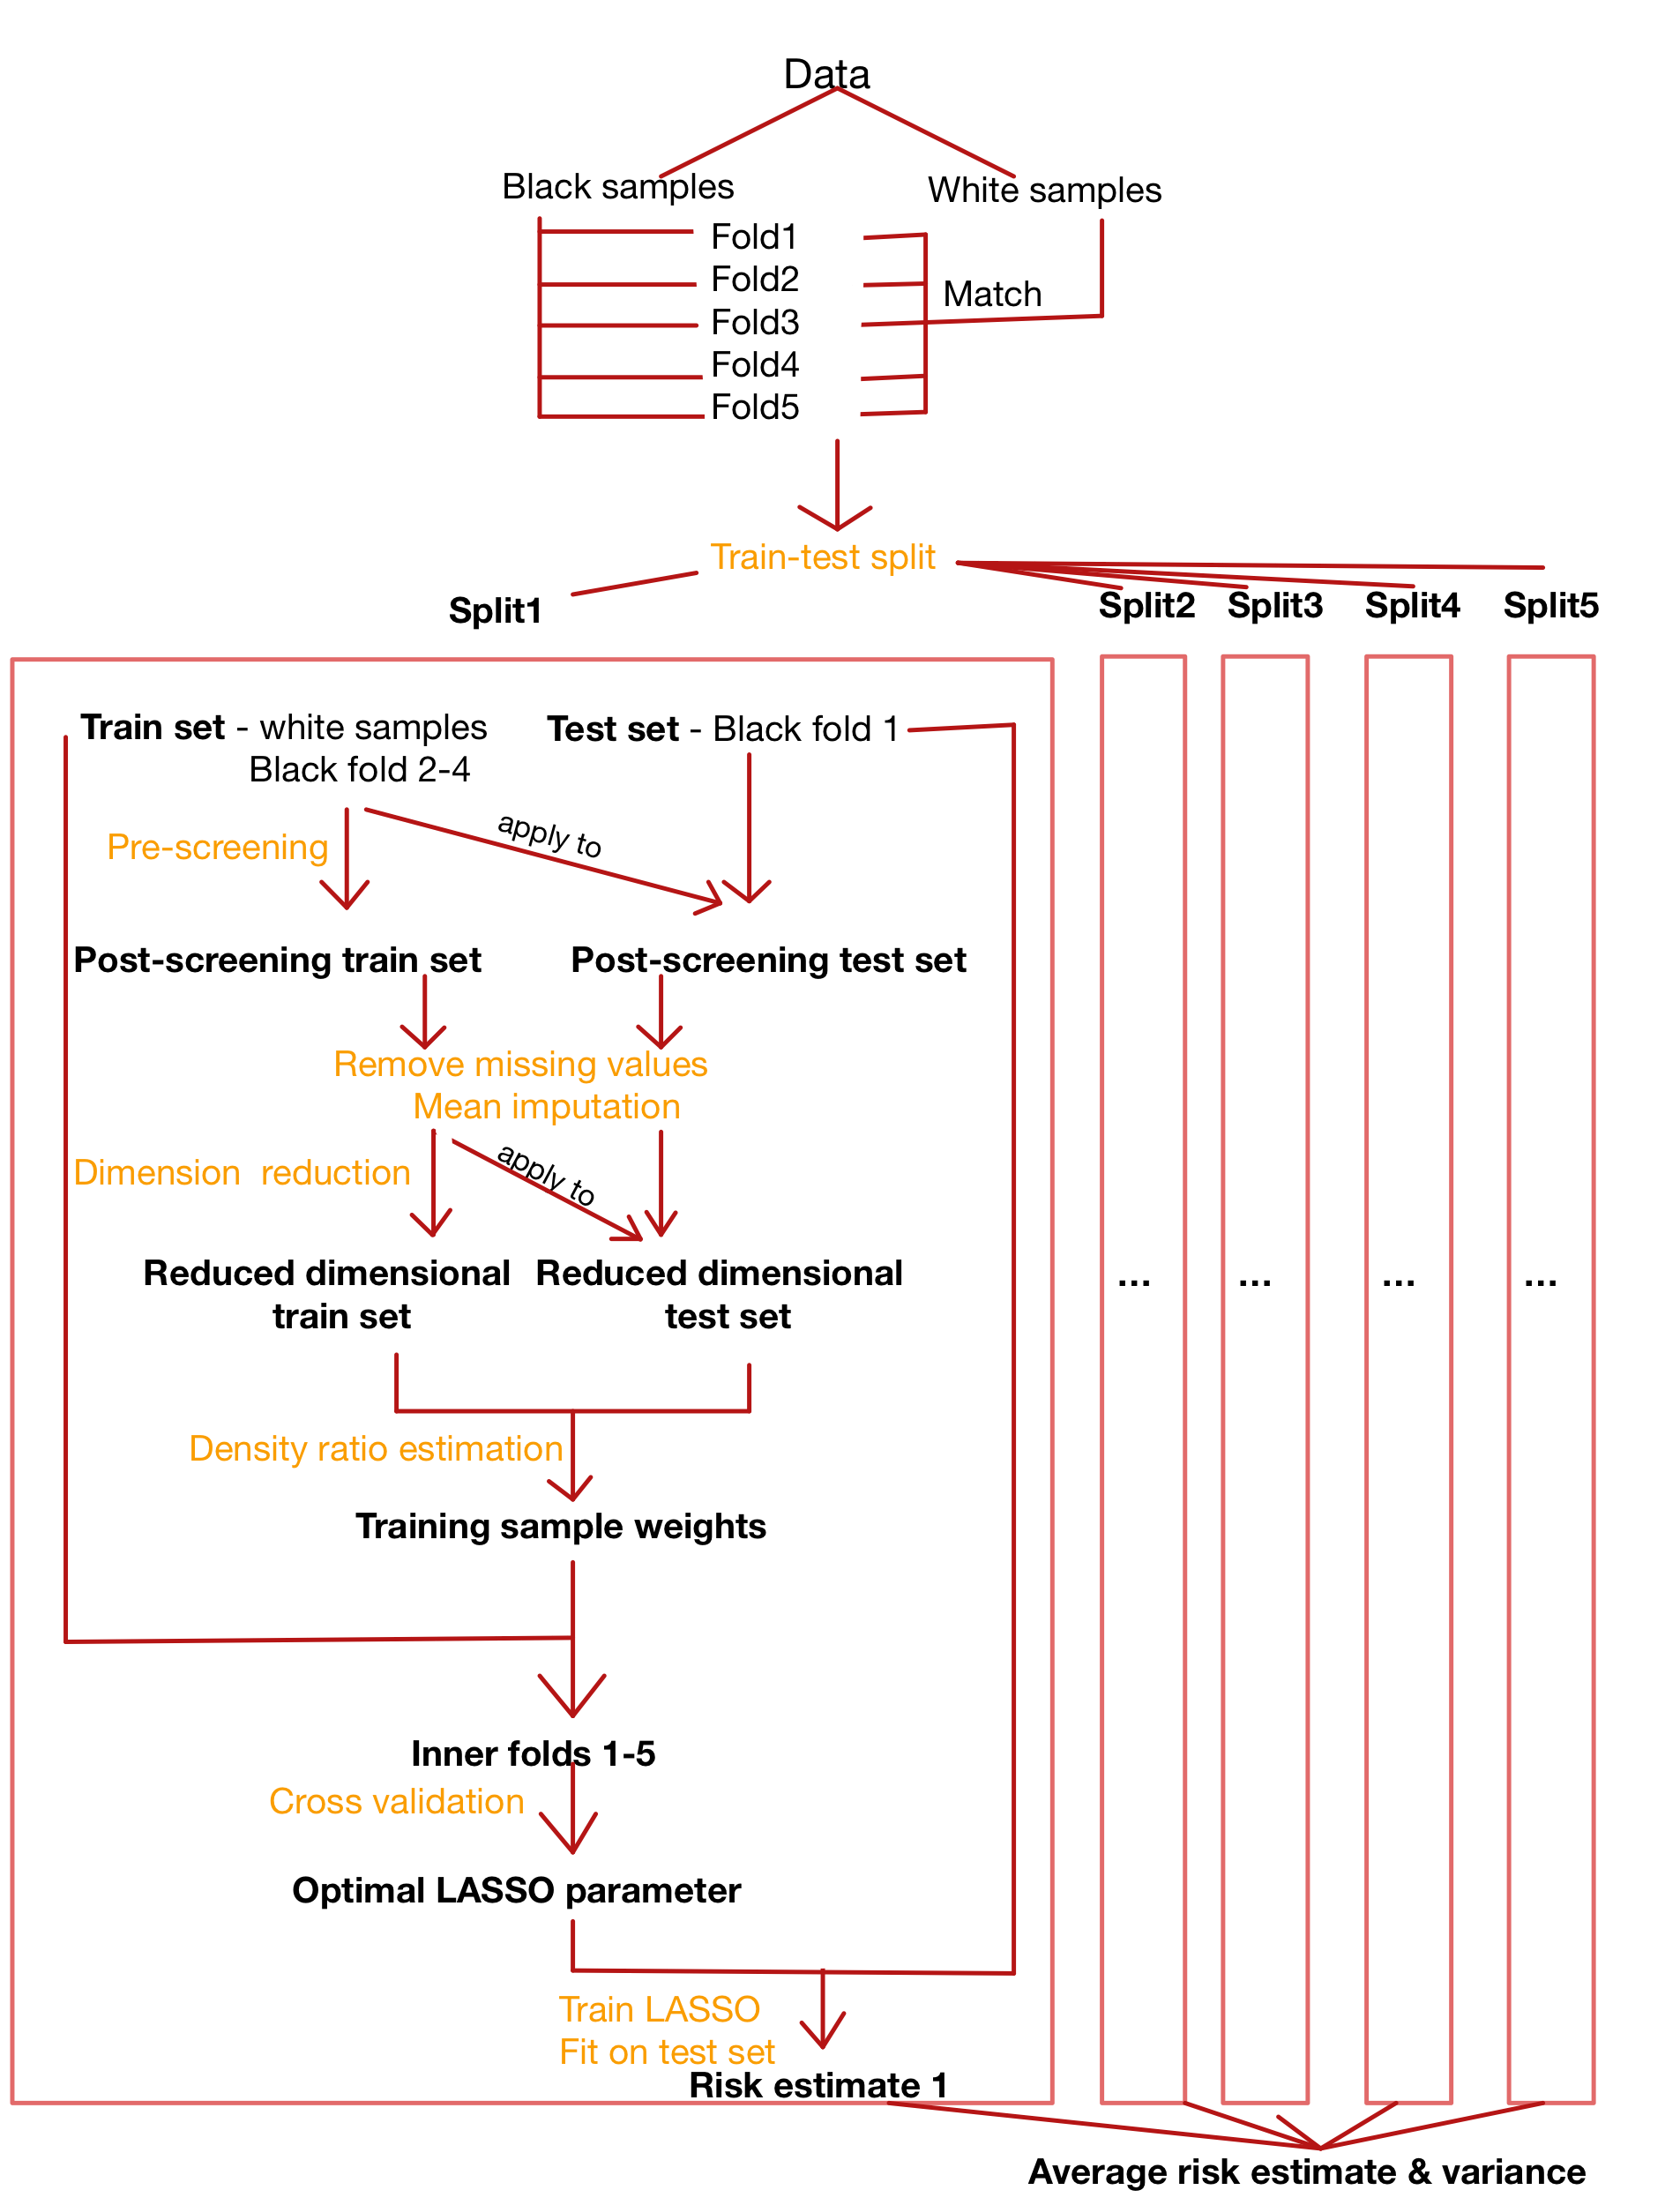
\includegraphics[width=\textwidth,height=\textheight,keepaspectratio]{flow chart.png}
    \caption{The design of experiment.}
    \label{experiment png}
\end{figure}
\pagebreak

\subsection{Results} \label{bio res}
We use the AUC as our main evaluation metric since it considers all possible decision thresholds. In medical diagnosis, one scientific interest is to find an optimal threshold that balances the sensitivity (probability of being test positive when disease is present) and specificity (probability of being test negative when disease is absent). A possible solution is to select one that maximises the Youden's $J$ statistic, defined as $$J = sensitivity + specificity - 1.$$
This cutoff point maximises the difference between the true positive rate and the false positive rate. With this threshold, we further report each model's sensitivity, specificity and accuracy. The results are summarised in Table \ref{final table} and Figure \ref{final figure} shows density plots for each set of weight estimates.

\begin{table}[H]
	\centering
\begin{tabular} {c | c | c | c | c }
method & AUC & sensitivity & specificity & accuracy  \\
\hline \hline
 \textbf{default} (5) & 0.568 (0.018) & 0.554 (0.133) & 0.642 (0.133) & 0.639 (0.128) \\
 KSPCA + KMM (2) & 0.546 (0.018) & 0.529 (0.195) & 0.699 (0.151) & 0.694 (0.141) \\
 KSPCA + KLIEP (4) & 0.546 (0.020) & 0.593 (0.176) & 0.617 (0.163) & 0.579 (0.183) \\
 LFDA + KLIEP (4)& 0.564 (0.017) & 0.514 (0.114) & 0.672 (0.126) & 0.668 (0.120) \\
 SPCA + KLIEP (5) & 0.535 (0.056) & 0.633 (0.118) & 0.510 (0.144) & 0.480 (0.138) \\
 SPCA + KMM (4)& 0.525 (0.035) & 0.708 (0.269) & 0.431 (0.244) & 0.586 (0.223) \\
 SPCA + ULSIF (3)& 0.568 (0.023) & 0.405 (0.086) & 0.800 (0.068) & 0.791 (0.066) \\
\hline \hline
\end{tabular}	
\caption{Models' performance on the UK Biobank dataset. For each evaluation metric, the numbers in brackets indicate the standard deviation. The numbers in the first column after name of each algorithm correspond to the number of folds a model has prediction results. Due to numerical instability, for some models the LASSO did not converge on all 5 train-test splits.}
\label{final table}
\end{table}

We did not perform SNMF here since it requires to iterate over all genotypes to find the optimal weight matrix $W$ and type matrix $T$. Given the dimensionality of the Biobank dataset, it is computationally infeasible to implement it. The experiment results show that similar as in the simulated dataset, a number of methods, especially ones using KSPCA, tend to assign zero weights to a large proportion of training samples, which reduces the effective sample size and further leads to poor predictive performance. For this dataset, the only model that is comparable to the standard LASSO model applies SPCA along with ULSIF.  Although our model has a marginally larger standard deviation in AUC, it significantly outperforms the default setting in predictive accuracy, given that the decision threshold is chosen by the Youden's score. This is possibly because our model gives large weights (>5) to Black samples in the each training set. From the figures, the model LFDA + KLIEP tends to filter out unimportant training samples rather than strengthening the Black samples in the training data, hence it has a narrow range of weights estimates without either large or small values.

The genotypes are likely to be correlated and the features post-screening can be similar to each other, hence numerical instability are observed during the implementation of these methods. For example, the within-sample covariance in LFDA and the kernel matrix in both KSPCA and KMM are occasionally nearly singular. The idea is to add a small constant, for example $10^{-6}$, which works as a regulariser to the diagonal elements of these matrices if their determinants are almost 0. However, during the implementation, we have spotted that the smallest constant needed to make these matrices positive definite can be up to the magnitude of $10^{-1}$, which greatly affects the results and sometimes leads to unreliable weight estimates. Another possible approach is to find the nearest positive definite matrix via the alternating projection method [\cite{higham2002computing}], but the computational requirement for working on such giant matrices makes it less effective in this application.

Secondly, the density plots demonstrate that the weights for Black samples do not appear to be significantly larger than the White samples, although the former exhibits more similar characteristics to the test set samples. This is possibly because the dimensionality of the feature reduced space is too small. For example, in SPCA and KSPCA, we keep the number of transformed covariates up to the threshold that 95\% of dependency of the phenotypes against genotypes is explained. This maps the original features onto a one-dimensional space. Also in other methods, the reduced dimension is normally less than 5. Thus, the feature mapping might have reduced the dissimilarity between samples from different populations and subsequently causes the density-ratio estimation methods to perform ineffectively. 

Also during the implementation, the LASSO regressions are fitted with the R package GLMNET [\cite{friedman2009glmnet}] which applies a second-order approximation at the beginning of each iteration and then apply a cyclic coordinate descent method to minimise a quadratic function. However, there is no guarantee that GLMNET converges to an optimum and this issue is encountered during our implementation, causing numerous models fail to provide results. Our initial guess was the large variance of the weight estimates causes numerical instability. Thus, we have carried out separate trials where the weights are exponentially flattened, then we imposed an upper limit such that the maximal weights do not exceed 5, we further centred the weights such that their means equal one. Even with these measures, the LASSO was still unable to converge. [\cite{yuan2010comparison}] compares various softwares for solving L1-regularised classifiers, then states that due to the approximation procedure employed throughout the GLMNET implementation, it is less stable than coordinate descent methods in training large-scaled datasets. To tackle the convergence problem, one needs to modify the Fortran code which the GLMNET is implemented upon, however, this is beyond the scope of our research interest.

\begin{figure}[H]
\begin{subfigure}{.32\textwidth}
  \centering
  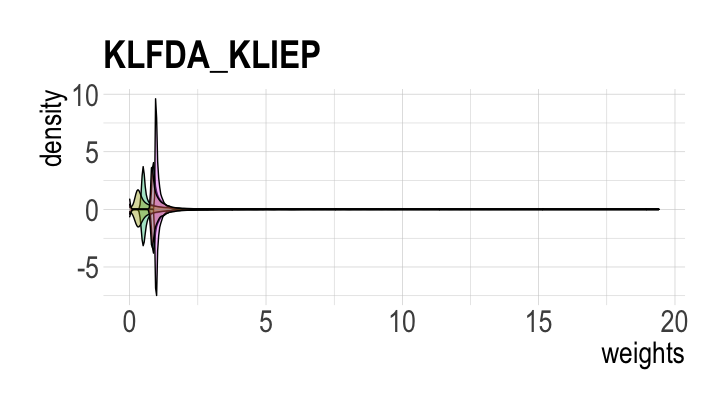
\includegraphics[width=\linewidth]{bio1.png}
  \label{fig:sfig1}
\end{subfigure}
\begin{subfigure}{.32\textwidth}
  \centering
  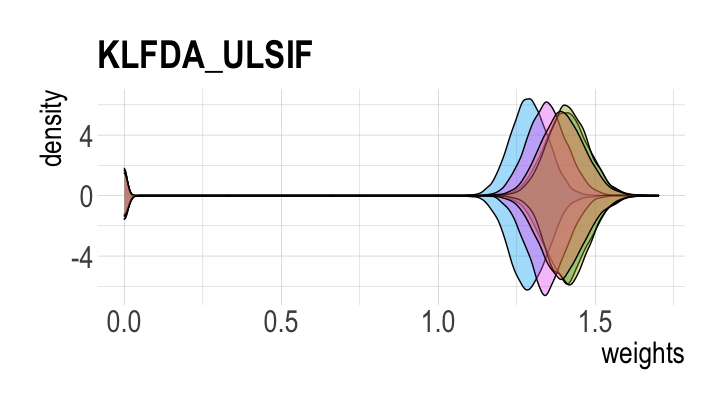
\includegraphics[width=\linewidth]{bio2.png}
  \label{fig:sfig2}
\end{subfigure} 
\begin{subfigure}{.32\textwidth}
  \centering
  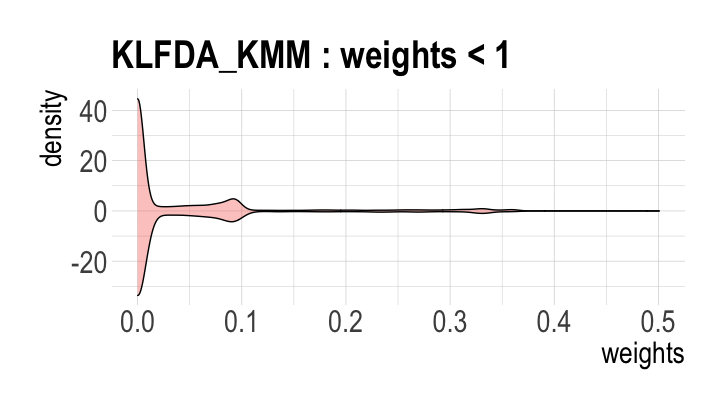
\includegraphics[width=\linewidth]{bio8.png}
  \label{fig:sfig1}
\end{subfigure}
\begin{subfigure}{.32\textwidth}
  \centering
  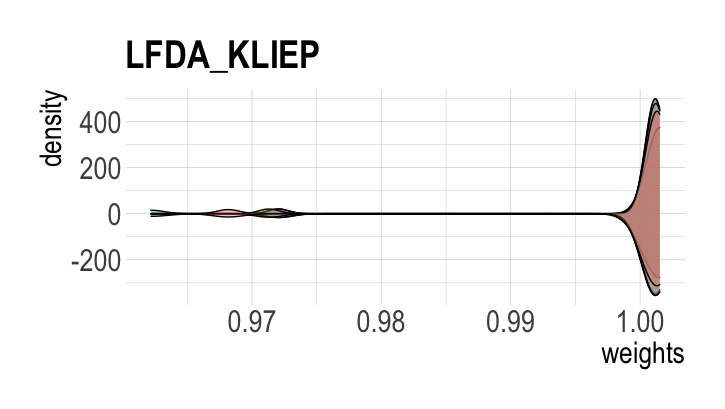
\includegraphics[width=\linewidth]{bio7.png}
  \label{fig:sfig2}
\end{subfigure} %
\begin{subfigure}{.32\textwidth}
  \centering
  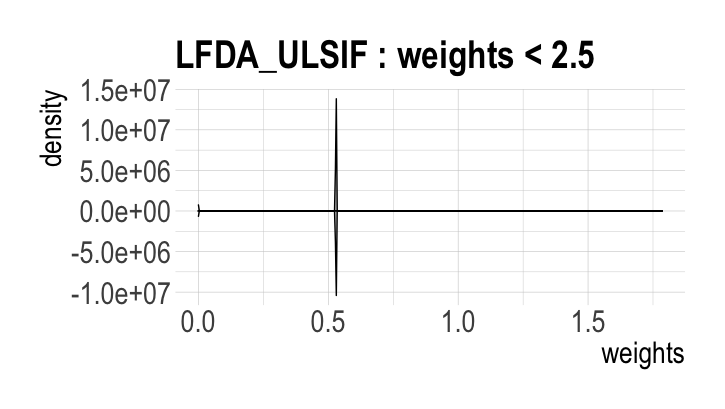
\includegraphics[width=\linewidth]{bio12.png}
  \label{fig:sfig1}
\end{subfigure}%
\begin{subfigure}{.32\textwidth}
  \centering
  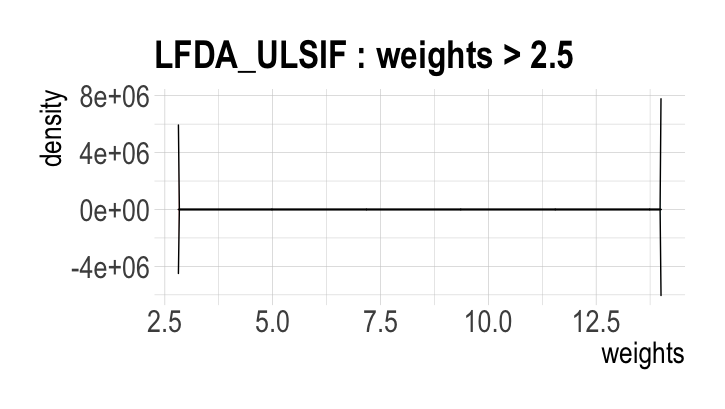
\includegraphics[width=\linewidth]{bio13.png}
  \label{fig:sfig2}
\end{subfigure} 
\begin{subfigure}{.32\textwidth}
  \centering
  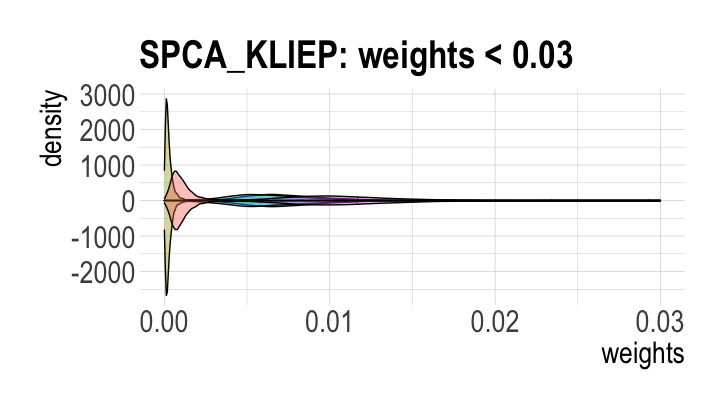
\includegraphics[width=\linewidth]{bio3.png}
  \label{fig:sfig1}
\end{subfigure}
\begin{subfigure}{.32\textwidth}
  \centering
  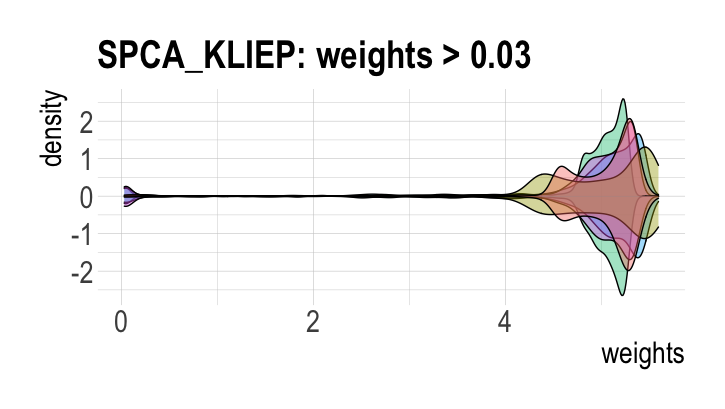
\includegraphics[width=\linewidth]{bio4.png}
  \label{fig:sfig2}
\end{subfigure} 
\begin{subfigure}{.32\textwidth}
  \centering
  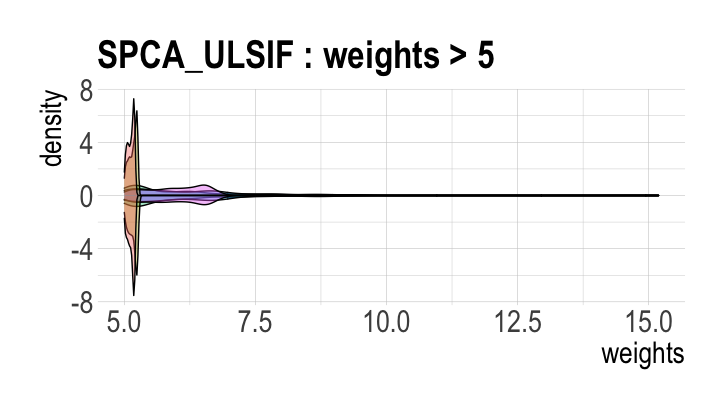
\includegraphics[width=\linewidth]{bio5.png}
  \label{fig:sfig1}
\end{subfigure}
\begin{subfigure}{.32\textwidth}
  \centering
  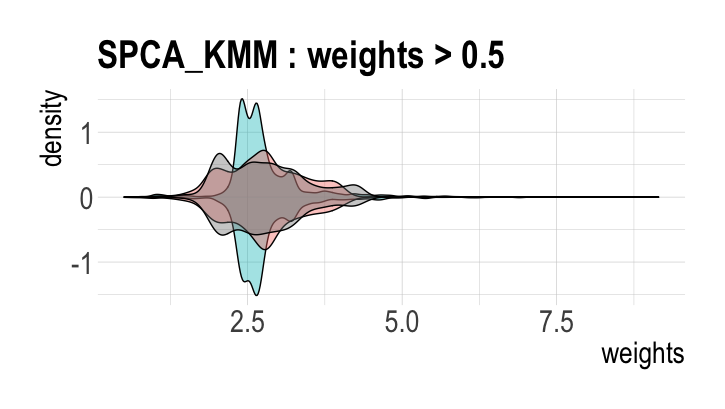
\includegraphics[width=\linewidth]{bio9.png}
  \label{fig:sfig2}
\end{subfigure} %
\begin{subfigure}{.32\textwidth}
  \centering
  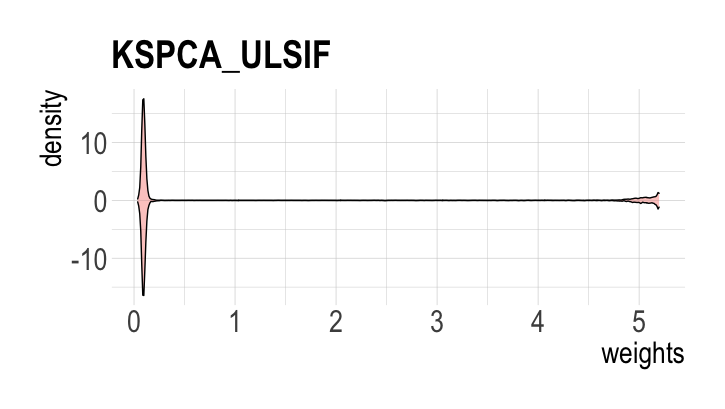
\includegraphics[width=\linewidth]{bio6.png}
  \label{fig:sfig1}
\end{subfigure}%
\begin{subfigure}{.32\textwidth}
  \centering
  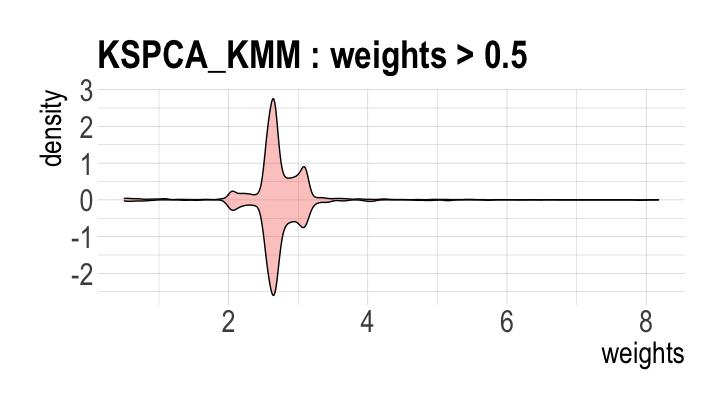
\includegraphics[width=\linewidth]{bio10.png}
  \label{fig:sfig2}
\end{subfigure} 
\begin{subfigure}{.32\textwidth}
  \centering
  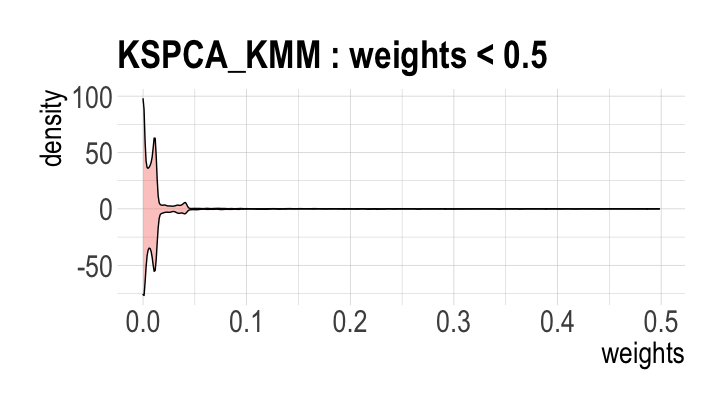
\includegraphics[width=\linewidth]{bio11.png}
  \label{fig:sfig2}
\end{subfigure} %
\begin{subfigure}{.32\textwidth}
  \centering
  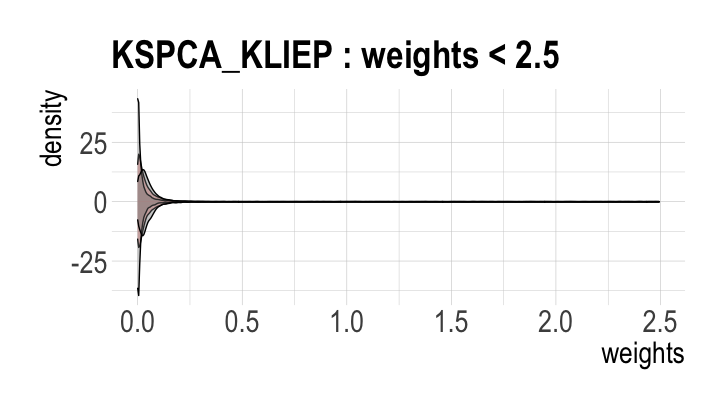
\includegraphics[width=\linewidth]{bio14.png}
  \label{fig:sfig1}
\end{subfigure}%
\begin{subfigure}{.32\textwidth}
  \centering
  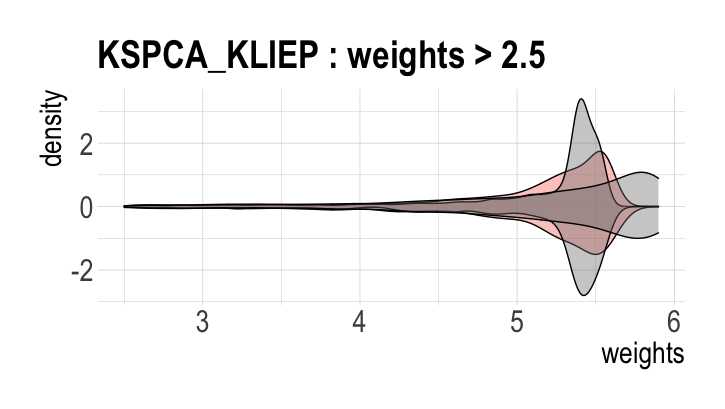
\includegraphics[width=\linewidth]{bio15.png}
  \label{fig:sfig2}
\end{subfigure} %
\caption{Density plots for weight estimates. Each colour represents a train-test split, the upper half of the plots shows the weights for the White individuals (account for approximately 80\% of training samples), the lower half shows weights for the Black samples. For a clear visualisation, models SPCA + KLIEP, KSPCA + KMM, KSPCA + KLIEP and LFDA + ULSIF are each split into two subfigures with different scale on the y-axis. For SPCA + ULSIF, the plot here only shows weights that are greater than 5, this counts for about 10\% of total training samples, the rest 90\% are close to 0. Similarly for SPCA + KMM, this plot only shows the top 20\% of weight estimates, the remaining are zeroes. }
\label{final figure}
\end{figure} 



%
%
%
%
\pagebreak
\section{Further Work} \label{Further Work}
In the pre-screening stage, we use univariate linear regressions asa from of supervised dimension reduction. This assumes that the variants are independent from each other, which is in general not true in a genotype dataset. In an extreme case, if only 1 genotype is statistically significant while all others are highly correlated to it, the current pre-screening approach would identify all genotypes as important ones. Hence, it may worth attempting more  sophisticated algorithm that accounts for the correlation structure between genotypes, such as Guided Regularised Random Forest [\cite{deng2013gene}].

For SDR, some machine learning/deep reduction methods such as autoencoder and variational autoencoder may be able to capture useful information about the structure of the genotypes. Supervised variants may also enhance predictive performace [\cite{ghosh2020supervised}, \cite{le2018supervised}].

The existing GLMNET implementation lacks theoretical convergence properties and may be ineffective in solving high dimensional problems. [\cite{yuan2012improved}] proposed an improved GLMNET which finds an optimal solution by firstly incorporating the coordinate descent approach, followed by the Newton method. The asymptotic convergence is guaranteed,  making it potentially more useful for large-scaled genomics datasets.

In this report, the proportion participants from the minority group in each training set was fixed at 20\%. If the LASSO logistic regression can converge properly, further work could examine how the performance of our density ratio estimation techniques change with this proportion. Similarly, one could vary the number of variants selected in the pre-screening stage, then apply use the same models to assess whether our algorithms can still work effectively across various dimensionality. 

In this work, we estimate the sample importance in the reduced dimension space, then fit a LASSO logistic regression on the original feature space. An alternatively worth consideration would be to both estimate the weights and fit the LASSO in the lower dimensional space. Given that we have abundant samples and features, some deep learning algorithms can possibly be applied to predict disease risks. For example, we can use Conv1D to reduce the dimensionality of features, followed by a LSTM to learn the sequential pattern of the dimension-reduced genotypes, then build classification models upon these results.

\pagebreak
\section{Conclusion} \label{Conclusion}
This work aims solve the problem that the training samples and the test samples differ in distributions by sample importance reweighting. We firstly introduced three density-ratio estimation methods - KMM, KLIEP and uLSIF - then illustrate that the performance of these models worsens when the dimensionality of features grows. Hence, we discussed a range of supervised dimension reduction methods, including SPCA, KSPCA, LFDA, KLFDA and SNMF. Then we implemented the above algorithms to a simulated genotyping dataset as well as the UK Biobank dataset. The results show that when applying to high dimensional datasets with complicated correlation structures, the algorithms may become numerically unstable, followed by a discussion about the possible reasons for this instability. Among those models that are computable, they marginally outperformed the standard LASSO logistic regression. Finally, we outlined the potential directions for improving the current designs.


%
%
%
%=============================================================
% the end
%=============================================================


\pagebreak
\bibliographystyle{apalike}
\bibliography{reference}
\pagebreak


\appendix
\begin{appendices}
The following provides important R functions for implementing methods introduced in this report. 

The full code can be found in: \url{https://github.com/shliu99/MSc-project-in-covariate-shift}
\section{R code: Pre-screening} \label{Appendix A}
\begin{lstlisting}[language=R]
# Estimate the p-value for each genotype in each train-test split
# load libraries
library(devtools)
library(snpnet)
library(readr)
library(dplyr)
library(parallel)

# set up parameters 
plink2_path  <- "/apps/eb/skylake/software/PLINK/2.00a2.3_x86_64/plink2"
zstdcat_path <- "/apps/eb/skylake/software/zstd/1.4.4-GCCcore-8.3.0/bin/zstdcat"
pheno  <- "breast"
prop   <- 0.2
nfolds <- 5

# use parallel computing
cl = parallel::makeCluster(detectCores())

# loop over all 5 train-test splits
for (fold in 1:nfolds) {
  kfile  <- file.path("data",
                      pheno,
                      paste0("fold", fold),
                      paste0("prop", prop, ".txt"))
  pfile  <- "data/all_vars.tsv"
  gfile  <- "data/ukb_cal_pgen/ukb_cal_all"
  covars <-
    c("Sex", "Age", paste0("PC", 1:10), paste0("PC", 1:10, "_Sex"))
  configs <- list(
    results.dir = file.path("temp", pheno,
                            paste0("fold", fold),
                            paste0("prop", prop)),
    plink2.path = plink2_path,
    zstdcat.path = zstdcat_path,
    keep = kfile
  )
  
  train_ids <- read.table(kfile)[, 1]
  ntrain <- length(train_ids)
  
  ids <- readIDsFromPsam(paste0(gfile, ".psam"))
  id_df <- data.frame(ID = ids, stringsAsFactors = F) %>%
    mutate(sort_order = 1:n())
  
  ### pre-screening
  
  phe <- readPheMaster(
    phenotype.file = pfile,
    psam.ids = ids,
    family = NULL,
    covariates = covars,
    phenotype = pheno,
    status = NULL,
    split.col = NULL,
    configs = configs
  ) 
  # for shell command
  # vars <- dplyr::mutate(dplyr::rename(
  #   data.table::fread(cmd=paste0(configs[['zstdcat.path']], ' ',
  #                                paste0(pfile, '.pvar.zst'))), 'CHROM'='#CHROM'),
  #   VAR_ID=paste(ID, ALT, sep='_'))$VAR_ID
  # n_genotypes <- length(vars)
  
  # for an R interactive session
  vars <-
    dplyr::mutate(dplyr::rename(data.table::fread(cmd = paste0(
      zstdcat_path, ' ', paste0(gfile, '.pvar.zst')
    )), 'CHROM' = '#CHROM'),
    VAR_ID = paste(ID, ALT, sep = '_'))$VAR_ID
  n_genotypes <- length(vars)
  
  
  
  pvar <- pgenlibr::NewPvar(paste0(gfile, '.pvar.zst'))
  pgen <- pgenlibr::NewPgen(paste0(gfile, '.pgen'),
                            pvar = pvar,
                            sample_subset = match(phe$ID, ids))
  data.y <- phe[[pheno]]
  # genotype data
  if (pheno == "breast" | pheno == "prostate") {
    data.X.gen2 <- as.matrix(cbind(data.y, Age = phe$Age,
                                   phe[, paste0("PC", 1:10)]))
  } else{
    data.X.gen2 <-
      as.matrix(cbind(
        data.y,
        Age = phe$Age,
        Sex1 = ifelse(phe$Sex == 1, 1, 0),
        Sex0 = ifelse(phe$Sex == 0, 1, 0),
        phe[, paste0("PC", 1:10)],
        phe[, paste0("PC", 1:10, "_Sex")]
      ))
  }
  
  
  # fit lm on variant ~ phe + sex + age + pc + pc*sex
  p = ncol(data.X.gen2)
  n = nrow(data.X.gen2)
  XtX.inv = solve(t(data.X.gen2) %*% data.X.gen2)
  XtX.inv.Xt =  XtX.inv %*% t(data.X.gen2)
  
  prescreening <-
    function(col,
             data.X.gen2,
             p,
             n,
             XtX.inv,
             XtX.inv.Xt) {
      col = matrix(col, ncol = 1)
      beta.hat = matrix(XtX.inv.Xt %*% col, ncol = 1)
      RSS = t(col - data.X.gen2 %*% beta.hat) %*% (col - data.X.gen2 %*% beta.hat)
      sigma2.hat = as.numeric(RSS / (n - p))
      beta.var = XtX.inv[1, 1] * sigma2.hat
      p.val = 2 * pt(abs(beta.hat[1] / sqrt(beta.var)),
                     df = (n - p),
                     lower.tail = F)
      return(p.val)
    }
  
  p.vals = vector("numeric")
  
  ### parallel computing
  count = 0
  n_each_time = 5000
  
  while (count +  n_each_time <= n_genotypes) {
    data.X.train <- pgenlibr::ReadList(pgen, 1:5000, meanimpute = T)
    p.vals = append(
      p.vals,
      parallel::parApply(
        cl,
        data.X.train,
        MARGIN = 2,
        prescreening,
        data.X.gen2 = data.X.gen2,
        p = p,
        n = n,
        XtX.inv = XtX.inv,
        XtX.inv.Xt = XtX.inv.Xt
      )
    )
    count <- count +  n_each_time
    cat(paste("current sample: ", count))
  }
  
  if (count +  n_each_time > n_genotypes) {
    data.X.train <-
      pgenlibr::ReadList(pgen, (count + 1):n_genotypes, meanimpute = T)
    p.vals = append(
      p.vals,
      parallel::parApply(
        cl,
        data.X.train,
        MARGIN = 2,
        prescreening,
        data.X.gen2 = data.X.gen2,
        p = p,
        n = n,
        XtX.inv = XtX.inv,
        XtX.inv.Xt = XtX.inv.Xt
      )
    )
  }
  
  features_selected = matrix(NA, ncol = 2, nrow = n_genotypes)
  colnames(features_selected) = c("inx", "p.val")
  features_selected[, 1] = 1:n_genotypes
  features_selected[, 2] = p.vals
  features_selected <-
    features_selected[order(features_selected[, 2]), ]
  outfile = file.path("data",
                      pheno,
                      paste0("fold", fold),
                      paste0("prop", prop, "_pvals.txt"))
  write(t(features_selected), outfile, ncolumns  = 2)
  rm(p.vals, features_selected)
}

parallel::stopCluster(cl)
\end{lstlisting}
\pagebreak

\section{R code: kernel functions and kernel parameter tuning} \label{Appendix B}
\begin{lstlisting}[language=R]
# function(1) and function(2) are stored in a script named "fun_kernel.R"
# Users need to source this file when implement SDR methods

###############################################################
# (1) rbfkernel function - default sigma = median distance
rbfkernel <- function(X, sigma = NULL, Y = NULL) {
  if (!is.matrix(X))
  {
    print("X must be a matrix containing samples in its rows")
    return()
  }
  if (!is.null(Y)) {
    if (!is.matrix(Y))
    {
      print("Y must be a matrix containing samples in its rows or 
      		NULL if it should not be used")
      return()
    }
    if (ncol(X) != ncol(Y)) {
      print("The samples in the rows of X and Y must be of same dimension")
      return()
    }
  }
  n <- nrow(X)
  if (is.null(Y)) {
    XtX <- tcrossprod(X)
    XX <- matrix(1, n) %*% diag(XtX)
    D <- XX - 2 * XtX + t(XX)
    if (is.null(sigma)) {
      sigma = var(D)
    }
  }
  else{
    m <- nrow(Y)
    XX <- matrix(apply(X ^ 2, 1, sum), n, m)
    YY <- matrix(apply(Y ^ 2, 1, sum), n, m, byrow = TRUE)
    XY <- tcrossprod(X, Y)
    D <- XX - 2 * XY + YY
    if (is.null(sigma)) {
      sigma = var(D)
    }
  }
  # calculate rbf-kernel matrix
  K <- exp(-D / (2 * sigma))
  return(K)
}

#(2) function for linear kernel
linearkernel <- function(X, Y = NULL){
  X = as.matrix(X)
  if(is.null(Y)){
    out <- tcrossprod(X,X)
  } else{
    out <- tcrossprod(X, Y)
  }
  return(out)
}
\end{lstlisting}
\pagebreak

\section{R code: tuning Gaussian kernel parameters} \label{Appendix B}
\begin{lstlisting}[language=R]
rbfkernel_cv <- function(X, sigma_lst, Y = NULL, lab) {
  if (!is.matrix(X))
  {
    print("X must be a matrix containing samples in its rows")
    return()
  }
  if (!is.null(Y)) {
    if (!is.matrix(Y))
    {
      print("Y must be a matrix containing samples in its rows or 
      		NULL if it should not be used")
      return()
    }
    if (ncol(X) != ncol(Y)) {
      print("The samples in the rows of X and Y must be of same dimension")
      return()
    }
  }
  lab = as.numeric(lab) + 1
  n <- nrow(X)
  if (is.null(Y)) {
    XtX <- tcrossprod(X)
    XX <- matrix(1, n) %*% diag(XtX)
    D <- XX - 2 * XtX + t(XX)
  }
  else{
    m <- nrow(Y)
    XX <- matrix(apply(X ^ 2, 1, sum), n, m)
    YY <- matrix(apply(Y ^ 2, 1, sum), n, m, byrow = TRUE)
    XY <- tcrossprod(X, Y)
    D <- XX - 2 * XY + YY
  }
  # calculate rbf-kernel matrix
  cv.res = matrix(NA, nrow = 2, ncol = length(sigma_lst))
  cv.res[1, ] = sigma_lst
  for (sigma in sigma_lst) {
    K <-  exp(-D / (2 * sigma))
    withinSum <-  0
    num = matrix(0, 1, max(lab))
    for (i in 0:max(lab)) {
      index <- lab == i
      withinSum <-  withinSum + sum(K[index, index])
      num[i] <-  sum(index)
    }
    betweenSum <-  sum(K) - withinSum
    withinNum <-  sum(num ^ 2)
    betweenNum <-  sum(num) ^ 2 - withinNum
    w <-  withinSum / withinNum
    b <-  betweenSum / betweenNum
    j <-  1 - w + b
    cv.res[2, which(sigma_lst %in% sigmalibrary("class")
\end{lstlisting}
\pagebreak

\section{R code: tuning dimension reduction methods parameters} \label{Appendix B}
\begin{lstlisting}[language=R]
library("lfda")
source("scripts/fun_lfda.R")

N = 1000
set.seed(10)
data.cv = sample(1:ntrain, 1000)
data.X.train = data.X.train[data.cv, ]
train.inx = list()
test.inx = list()
inx = split(seq_len(N), cut(seq_len(N), breaks = 5))
for (i in 1:5) {
  train.inx[[i]] = seq_len(N)[!(seq_len(N) %in% inx[[i]])]
  test.inx[[i]] = inx[[i]]
}

dim.lst = c(10, 100, 300, 500)
mis.class.error = matrix(NA, ncol = 5, nrow = length(dim.lst))
rownames(mis.class.error) = dim.lst
colnames(mis.class.error) = paste0("foldi", 1:5)

for (foldi in 1:5) {
  data.X.train.cv = data.X.train[train.inx[[foldi]], ]
  data.X.test.cv = data.X.train[test.inx[[foldi]], ]
  data.y.cv = data.y[train.inx[[foldi]]]
  data.y.test = data.y[test.inx[[foldi]]]
  for (dim in dim.lst) {
    lfda.res <- lfda(data.X.train.cv,
                     data.y.cv,
                     dim,
                     knn = 7 ,
                     metric = "orthonormalized")
    X.train.lfda <- predict(lfda.res, data.X.train.cv)
    X.test.lfda <- predict(lfda.res, data.X.test.cv)
    knn.res = knn1(X.train.lfda, X.test.lfda, data.y.cv)
    mis.rate = sum(knn.res != data.y.test) / length(knn.res)
    mis.class.error[which(dim.lst %in% dim), foldi] = mis.rate
    cat(paste(
        "the misclassification rate for cv fold ", foldi,
        "dimension ",dim,
        "is", mis.rate,"\n"))
}}
      
\end{lstlisting}
\pagebreak

\section{R code: supervised dimension reduction} \label{Appendix B}
\begin{lstlisting}[language=R]
###############################################################
# (1) function for supervised PCA - primal
library(rARPACK)
source("scripts/fun_kernel.R")

spca <- function(X,Y, prop = 0.95){
  if(!is.matrix(X)){
    X = as.matrix(X)
  }
  X = t(X)
  n = ncol(X)
  L = linearkernel(Y)
  H = diag(n) - 1/n * outer(rep(1,n), rep(1,n))
  Q = X %*% H %*% L %*% H %*% t(X)
  if(det(Q) == 0){
    Q = Q + diag(1e-6,nrow(X))
  }
  eig.vals <- eigen(Q, only.values = TRUE)$values
  pc_n <- length(which(cumsum(eig.vals^2)/sum(eig.vals^2) <= 0.95)) + 1
  beta <- eigs(Q, k = pc_n, which = "LM")$vectors
  return(beta)
}

###############################################################
# (2) function for supervised PCA - improved efficiency on svd
library(rARPACK)
source("scripts/fun_kernel.R")

spca <- function(X,Y, prop = 0.95){
  if(!is.matrix(X)){
    X = as.matrix(X)
  }
  X = t(X)
  n = ncol(X)
  L = linearkernel(Y)
  eig = eigen(L)
  rm(L)
  delta = t(eig$vectors %*% diag(sqrt(ifelse(eig$values >= 0, eig$values, 0))))
  H = diag(n) - 1/n * outer(rep(1,n), rep(1,n))
  psi = X %*% H %*% t(delta)
  svd_sing <- svd(psi, nu = 0, nv = 0)$d
  pc_n <- length(which(cumsum(svd_sing^2)/sum(svd_sing^2) <= prop)) + 1
  v = svds(psi, k = pc_n, nu = 0, nv = pc_n)$v
  if(pc_n >= 2){
    u <- psi %*% v %*% diag(1 / svd_sing[1:pc_n])
  } else{
    u <- psi %*% v %*% (1 / svd_sing[1:pc_n])
  }
  return(u)
}

# both function(1) and function(2) are supervised PCA, function(1) 
# uses the primal optimisation formulation, which does not require
# matrix decomposition, but need to store an n*n matrix; function(2)
# uses a p*p kernel matrix, but extra computations required for LU
# decomposition. The users need to find a balance between space
# complexity and time complexity, then choose the one that is more
# appropriate for their dataset.

###############################################################
# (3) function for kernel SPCA
source("scripts/fun_kernel.R")
library(rARPACK)

kSPCA <- function(X, Y, sigma){
  X = as.matrix(X); Y = as.matrix(Y)
  K = rbfkernel(X, sigma = sigma)
  L = linearkernel(Y)
  n = nrow(K)
  if(det(Q) == 0){
    K = K + diag(1e-6, n)
  }
  H = diag(n) - 1/n * outer(rep(1,n), rep(1,n))
  Q = K %*% L %*% H %*% K
  if(det(Q) == 0){
    Q = Q + diag(1e-6, n)
  }
  eig.vals <- eigen(Q, only.values = TRUE)$values
  pc_n <- length(which(cumsum(eig.vals)/sum(eig.vals) <= 0.95)) + 1
  beta <- eigs(Q, k = pc_n, which = "LM")$vectors
  return(beta)
}

###############################################################
# (4) function for lfda 
library("lfda")

lfda <- function (x,
                  y,
                  r,
                  metric = c("orthonormalized", "plain",
                             "weighted"),
                  knn = 7) {
  metric <- match.arg(metric)
  x <- t(as.matrix(x))
  y <- t(as.matrix(y))
  d <- nrow(x)
  n <- ncol(x)
  if (is.null(r))
    r <- d
  tSb <- mat.or.vec(d, d)
  tSw <- mat.or.vec(d, d)
  for (i in unique(as.vector(t(y)))) {
    Xc <- x[, y == i]
    nc <- ncol(Xc)
    Xc2 <- t(as.matrix(colSums(Xc ^ 2)))
    distance2 <- repmat(Xc2, nc, 1) + repmat(t(Xc2), 1, nc) -
      2 * t(Xc) %*% Xc
    A <- getAffinityMatrix(distance2, knn, nc)
    Xc1 <- as.matrix(rowSums(Xc))
    G <- Xc %*% (repmat(as.matrix(colSums(A)), 1, d) * t(Xc)) -
      Xc %*% A %*% t(Xc)
    tSb <- tSb + (G / n) + Xc %*% t(Xc) * (1 - nc / n) + Xc1 %*%
      (t(Xc1) / n)
    tSw <- tSw + G / nc
  }
  X1 <- as.matrix(rowSums(x))
  tSb <- tSb - X1 %*% t(X1) / n - tSw
  tSb <- (tSb + t(tSb)) / 2
  tSw <- (tSw + t(tSw)) / 2
  if (det(tSw) == 0) {
    tSw = tSw + diag(1e-6, d)
  }
  if (r == d) {
    eigTmp <- eigen(solve(tSw) %*% tSb)
  }
  else {
    eigTmp <- suppressWarnings(rARPACK::eigs(
      A = solve(tSw) %*%
        tSb,
      k = r,
      which = "LM"
    ))
  }
  eigVec <- Re(eigTmp$vectors)
  eigVal <- as.matrix(Re(eigTmp$values))
  Tr <- getMetricOfType(metric, eigVec, eigVal, d)
  Z <- t(t(Tr) %*% x)
  out <- list(T = Tr, Z = Z)
  class(out) <- "lfda"
  return(out)
}

###############################################################
# (5) function for kernel lfda 

library("lfda")
klfda <-
  function (k,
            y,
            r,
            metric = c("weighted", "orthonormalized",
                       "plain"),
            knn = 7,
            reg = 0.001) {
    metric <- match.arg(metric)
    y <- t(as.matrix(y))
    n <- nrow(k)
    if (is.null(r))
      r <- n
    tSb <- mat.or.vec(n, n)
    tSw <- mat.or.vec(n, n)
    for (i in unique(as.vector(t(y)))) {
      Kcc <- k[y == i, y == i]
      Kc <- k[, y == i]
      nc <- nrow(Kcc)
      Kccdiag <- diag(Kcc)
      distance2 <- repmat(Kccdiag, 1, nc) + repmat(t(Kccdiag),
                                                   nc, 1) - 2 * Kcc
      A <- getAffinityMatrix(distance2, knn, nc)
      Kc1 <- as.matrix(rowSums(Kc))
      Z <- Kc %*% (repmat(as.matrix(colSums(A)), 1, n) * t(Kc)) -
        Kc %*% A %*% t(Kc)
      tSb <- tSb + (Z / n) + Kc %*% t(Kc) * (1 - nc / n) + Kc1 %*%
        (t(Kc1) / n)
      tSw <- tSw + Z / nc
    }
    K1 <- as.matrix(rowSums(k))
    tSb <- tSb - K1 %*% t(K1) / n - tSw
    tSb <- (tSb + t(tSb)) / 2
    tSw <- (tSw + t(tSw)) / 2
    if (det(tSw) == 0) {
      tSw = tSw + diag(1e-6, n)
    }
    if (det(tSb) == 0) {
      tSb = tSb + diag(1e-6, n)
    }
    eigTmp <- suppressWarnings(rARPACK::eigs(
      A = solve(tSw +
                  reg * diag(1, nrow(tSw), ncol(tSw))) %*% tSb,
      k = r,
      which = "LM"
    ))
    eigVec <- Re(eigTmp$vectors)
    eigVal <- as.matrix(Re(eigTmp$values))
    Tr <- getMetricOfType(metric, eigVec, eigVal, n)
    Z <- t(t(Tr) %*% k)
    out <- list(T = Tr, Z = Z)
    class(out) <- "lfda"
    return(out)
  }

# (6) Supervised NMF
data.X.train <- data.X.train[,colSums(data.X.train)!=0]
data.X.test <- data.X.test[,colSums(data.X.test)!=0]
t_types <-  chty(data.X.train, data.y, 2, 3)
nmb1 <-  t_types$r1
nmb2 <-  t_types$r2
t_total <- getT(data.X.train,data.y,nmb1,nmb2)
X.train.out <- spnmf(data.X.train, t_total)$W
X.test.out <- spnmf(data.X.test, t_total)$W
\end{lstlisting}
\pagebreak

\section{R code: density ratio estimation} \label{Appendix B}
\begin{lstlisting}[language=R]
###############################################################
# (1) function for KMM
library("quadprog")
source("scripts/fun_kernel.R")
source("scripts/fun_gaussian_cv.R")

kmm <- function(x_tr, x_te) {
  x_tr = as.matrix(x_tr)
  x_te = as.matrix(x_te)
  n_tr = nrow(x_tr)
  n_te = nrow(x_te)
  sigma = kernelWidth_median(x_tr)
  # calculate kernel
  cat("computing kernel for training data... \n")
  Ktrtr = rbfkernel(x_tr, sigma = sigma)
  Xtrtr =
    if (det(Ktrtr) == 0) {
      Ktrtr = Ktrtr + diag(1e-6, n_tr)
    }
  # compute kappa
  cat("computing kappa... \n")
  Ktrte = rbfkernel(X = x_tr, Y = x_te, sigma = sigma)
  kappa = rowSums(Ktrte) * n_tr / n_te
  # compute epsilon
  cat("computing epsilon... \n")
  eps = (sqrt(n_tr) - 1) / sqrt(n_tr)
  # constraints
  Amat <-
    cbind(rep(-1, n_tr), rep(1, n_tr), diag(1, n_tr), diag(-1, n_tr))
  bvec <- c(-n_tr * (eps + 1),
            max(-n_tr * (eps - 1), 0),
            rep(0, n_tr),
            rep(-sqrt(n_tr) + 1, n_tr))
  # computing beta
  cat("computing beta... \n")
  beta = solve.QP(Ktrtr, kappa, Amat, bvec)$solution
  beta[beta < 0] = 0
  return(beta)
}

###############################################################
# (2) functions for KLIEP
library("densratio")
compute_kernel_Gaussian <- function(x, centers, sigma) {
  apply(centers, 1, function(center) {
    apply(x, 1, function(row) {
      kernel_Gaussian(row, center, sigma)
    })
  })
}

kernel_Gaussian <- function(x, y, sigma) {
  exp(- squared_euclid_distance(x, y) / (2 * sigma * sigma))
}

squared_euclid_distance <- function(x, y) {
  sum((x - y) ^ 2)
}

num <- nrow(X.test.out) * 0.5
kliep.obj <-
  densratio(X.test.out,
            X.train.out,
            method = "KLIEP",
            kernel_num = num)
weights <-
  compute_kernel_Gaussian(X.train.out,
                          kliep.obj$kernel_info$centers,
                          kliep.obj$kernel_info$sigma) %*% kliep.obj$kernel_weights

###############################################################
# (3) functions for uLSIF
num <- nrow(X.test.out) * 0.5
weights <-
  densratio(X.test.out,
            X.train.out,
            method = "uLSIF",
            kernel_num = num)$compute_density_ratio(X.train.out)
\end{lstlisting}

\pagebreak
\section{R code: evaluate the model performance}
\begin{lstlisting}
## evaluate UK biobank results 
library(readr)
library(pROC)

sdr = "spca"
dre = "ulsif"
weights_algo = paste(sdr, dre, sep = "_")

results <- matrix(NA, ncol = 7)
results = as.data.frame(results)
colnames(results) = c("algorithm", "fold", "auc", "threshold",
                      "sensitivity", "specificity", "accuracy")
for (fold in 1:5){
  res.path = file.path(paste0("fold", fold),
                       paste0(weights_algo,"_screen0.05_res.tsv"))
  preds = read_tsv(res.path)
  auc <- auc(preds$y, preds$pred_bin)
  # partial_auc <- auc(preds$y, preds$pred_bin, partial.auc = c(0,0.1),
  #                   partial.auc.correct = TRUE)
  roc.info <- roc(preds$y, preds$pred_bin)
  roc.df <- data.frame(sensitivity= roc.info$sensitivities,
                       specifity = roc.info$specificities,
                       threshold = roc.info$thresholds)
  roc.df$youden<- roc.df$sensitivity + roc.df$specifity - 1
  threshold.vals = roc.df[which(roc.df$youden == max(roc.df$youden)),]
  threshold <- threshold.vals$threshold
  labs <- ifelse(preds$pred_bin >= threshold, TRUE, FALSE)
  accurary <- sum(labs == preds$y)/nrow(preds)
  
  results <- rbind(results, c(weights_algo,
                              fold,
                              round(c(auc,
                              threshold,
                              threshold.vals$sensitivity,
                              threshold.vals$specifity,
                              accurary),3)))
}
\end{lstlisting}


\end{appendices}
\pagebreak

\end{document}
